\documentclass[12pt,a4paper]{book} 
%\documentstyle[11pt,a4,axodraw]{book}
%\documentclass[12pt,american,a4paper,twoside,openbib]{book}
%\usepackage[latin1]{inputenc}
%\usepackage[T1]{fontenc}
\usepackage[american]{babel}
%\usepackage{babel,lucbr}

\usepackage{axodraw}
\usepackage{epsfig,wrapfig,subfigure,graphicx}
\usepackage{subfigure}
\usepackage{amsmath, amscd, amssymb, latexsym, array}
%\usepackage{amsmath, amscd, intlim, amssymb, latexsym, array}  
\newcommand{\state}[3]{ ${}^{#1} \textrm{#2}_{#3}$ }
\newcommand{\statet}[3]{ {}^\textrm{#1} \textrm{#2}_\textrm{#3} } 
\newcommand{\SE}{\text{Schr$\ddot{\textrm{o}}$dinger equation}}
\newcommand{\LS}{\text{Lippmann-Schwinger}} 







\newlength{\head}

\font\tenrm=cmr10
\textheight 9in
\textwidth 6in
\oddsidemargin 1.0cm
\evensidemargin -0.15in
\topmargin -5pt
\newlength{\topp}
\setlength{\topp}{\textwidth}


\newcommand{\heading}[2]{\markboth{\settowidth{\head}
                        {Kapittel \arabic{chapter}. #1}
    \addtolength{\head}{1.5cm}
     \protect\hspace{-8mm}
     \protect\rule[-0.15cm]{\topp}{0.2mm}
     \protect\hspace{-\head}
     \bf{\hfill Chapter \arabic{chapter}. #1} }
     {\protect\rule[-0.15cm]{\topp}{0.2mm} 
     \protect\hspace{-\topp}
     \protect\hspace{-0.5cm}
     \protect\bf{ \arabic{chapter}.\arabic{section} \hspace{2mm} #2 \hspace{\fill} } }}
 
 
 
\newcommand{\headingx}[1]{\markboth{\settowidth{\head}{#1}
     \addtolength{\head}{1.5cm}
     \protect\hspace{-8mm}
     \protect\rule[-0.15cm]{\topp}{0.2mm}
     \protect\hspace{-\head}
     \bf{\hfill #1} }
     {\protect\rule[-0.15cm]
     {\topp}{0.2mm} \protect\hspace{-\topp}
     \protect\hspace{-0.5cm}
     \protect\bf{ #1\hspace{\fill}} }}

\newcommand{\headinga}[2]{\markboth{\settowidth{\head}{#1}
     \addtolength{\head}{1.2cm}
     \protect\hspace{-8mm}
     \protect\rule[-0.15cm]{\topp}{0.2mm}
     \protect\hspace{-\head}
     \bf{\hfill #1} }
     {\protect\rule[-0.15cm]
     {\topp}{0.2mm} \protect\hspace{-\topp}
     \protect\hspace{-0.5cm}
     \protect\bf{ \Alph{chapter}.\arabic{section} \hspace{2mm} #2} }} 
\newenvironment{innrykk}{\begin{itemize}}{\end{itemize}}

\newcommand{\bra}[1]{\ensuremath{\langle#1|}}
\newcommand{\ket}[1]{\ensuremath{|#1\rangle}}
\newcommand{\braket}[2]{\ensuremath{\langle#1|#2\rangle}}
\newcommand{\braketm}[3]{\ensuremath{\langle#1|#2|#3\rangle}} 
%\newcommand{\op}[1]{\ensuremath{\widehat{#1}}}
\newcommand{\opavg}[1]{\ensuremath{\langle\op{#1}\rangle}}
\newcommand{\vecdots}[2]{\ensuremath{\vec{x}_{#1},\dots,\vec{x}_{#2}}}
\newcommand{\prvecdots}[2]{\ensuremath{\vec{x}'_{#1},\dots,\vec{x}'_{#2}}}
\newcommand{\fdiff}[1]{\ensuremath{\frac{\delta#1[\rho]}{\delta\rho(\vec{r})}}}
\newcommand{\vr}{\ensuremath{\vec{r}}}
%\newcommand{\half}{\ensuremath{\frac{1}{2}}}
%\newcommand{\beq}{\begin{equation}}
%\newcommand{\beqla}[1]{\begin{equation}\label{#1}}
\newcommand{\eeq}{\end{equation}}
%\newcommand{\eqn}[1]{(\ref{#1})}
\newcommand{\dir}[1]{{\bf \op{#1}}}
\def\KeyWord#1{$\backslash$\IfColor{$\!\!$\textRed{#1}\textBlack}{#1}$\!\!$}


\newcommand{\halv}{\frac{1}{2}}
\newcommand{\inv}[1]{\frac{1}{#1}}
\newcommand{\Tr}{\text{Tr}}
\newcommand{\halve}[1]{\frac{#1}{2}}
\newcommand{\pil}{\rightarrow}
\newcommand{\dpil}{\Rightarrow}

\newcommand{\beg}{\begin{equation}\;}
\newcommand{\slutt}{\!\end{equation}}
\newcommand{\begm}[1]{\begin{equation}\label{#1}}
\newcommand{\lnr}[1]{lign.(\ref{#1})}
\newcommand{\nr}[1]{(\ref{#1})}

\newcommand{\yd}{\underline{d}}
\newcommand{\bform}{\underline{\omega}}
\newcommand{\rform}{\underline{\Omega}}
\newcommand{\kform}{\underline{R}}

\newcommand{\mpl}{M_P^{\;2}}
\newcommand{\op}[1]{\ensuremath{\hat{#1}}}
\newcommand{\rot}[1]{\sqrt{#1}}

\newcommand{\nl}{\newline\phantom{ekko}\newline}

\newcommand{\aaa}{{\aa}}

\newcommand{\kap}[1]{\chapter{#1}\def\kapnavn{#1}\heading{\kapnavn}{} }
\newcommand{\avsnitt}[1]{\section{#1}\heading{\kapnavn}{#1}}

\newcommand{\akap}[1]{\chapter{#1}\def\kapnavn{#1}\headinga{\kapnavn}{} }






%\usepackage{maple2e}
% \def\emptyline{\vspace{12pt}}
% \DefineParaStyle{Maple Output}
% \DefineParaStyle{Maple Plot}
% \DefineCharStyle{2D Math}
% \DefineCharStyle{2D Output}

\title{Theses In Nuclear Physics}
\author{Eivind Brodal}
\date{2002}

\begin{document}
\maketitle 

\tableofcontents

\kap{Introduction}\label{chap:innledning}
%\begin{flushleft}


\section[Nucleon-Nucleon models]{Nucleon-Nucleon(NN) interactions And Nuclear Models}



Particles can be grouped into three different categories, which are leptons, baryons and mesons.
Leptons are particles like the electron and neutrino. 
Baryons are particles with half integer spin like the nucleons,
while mesons are particles with integer spin.
It is also normal to call the big group of baryons and mesons for hadrons, since they are all made from quarks.

The mesons are the carrier of the strong force. They can interact with nucleons through the strong, weak,
electromagnetic and gravitational force. Free mesons can be produced in nucleon-nucleon collisions, but they decay
rapidly into lighter mesons, leptons or photons either through strong, weak or electromagnetic interactions. 
The decay lifetimes are around $10^{-20}-10^{-23}$ for strong decays, $10^{-16}-10^{-18}$ for electromagnetic decays 
and $10^{-8}-10^{-10}$ for weak decay. In the nucleon-nucleon scattering processes we are looking at, we can
neglect all the other forces except the strong force. So the contribution to the potential created between
the nucleons are  only arising from strong interactions through virtual meson exchange.

There are many different mesons. They all have their own contribution to the strong force,
which is a superposition from all the possible ways the mesons can be exchanged. 
i.e. not only a single meson exchange, but also more complicated events where two ore more mesons are transfered.
All the mesons have their own characteristic combination of mass, spin, parity, isospin and decay rate. 
these parameters are important for the range of the force, but also for where it will be repulsive/attractive.
It is normal to divide the range of the strong force into three regions; 
The short range, the intermediate region and the long-range of the force.
For example the $\pi$-meson as the lightest particle provides the long-range force. 
While the $\omega$-meson is responsible for the short-range repulsion, which explains the observed hard core of
the nucleons when they are squeezed together. From electron scattering experiments on heavy nuclears,
one have found an average distance between the centers of the nucleons to be 1.8 fm. 
This is a too large diameter of the hard core arising from the strong force. It turns out that the Pauli 
principal is more important for nucleons hard core observed in heavy nuclears. 
A better way to determine the hard core from the strong interaction is NN data form the \state{1}{S}{0}- phase shift.
This state is chosen since it doesn't have a centrifugal barrier. i.e. the angular orbital momentum; L=0. 
From fig~\ref{fig:manypotS} we see that the phase shift turns negative/repulsive around $E_{lab}=250$ MeV.
The maximum classical orbital angular momentum $L_{max}$ is
\begin{equation}\label{eq:Lmax}
L_{max}=Rp=R\sqrt{\frac{E_{lab}M}{2}}
\end{equation}
Where R is the range/radius of the hard core and M is the mass of the nucleon.
With $L\le1$ we obtain an estimate of the radius of the hard core: 
\begin{equation}\label{eq:Lmax2}
R\le 0.6 \text{ fm}
\end{equation}
Experiments shows that the deuterium has a magnetic moment, which means that the bound nuclei is a mixture
of the S-state (L=0) and the D-state (L=2). This indicates that the strong force also contains a tensor-force
that can couple the two states with the same good quantum numbers. 
%This indicates that we need more than 
%the Klein-Gordon equation, which is the relativistic wave equation for scalar fields. 
The Klein-Gordon equation is used to calculate a potential from mesons with spin-$0$ (Yukawa potentials).
The Yukawa potential has it origin from a scalar-force.
This indicates that we need to work with more than
the Klein-Gordon equation to reproduce the tensor-force.
%, which is the relativistic wave equation for scalar fields.
The Dirac equation on the other hand will be able of handling tensor-forces, 
but is only valid for half integer spin particles like nucleons and quarks.
One must of course use field theories for spin-1, spin-2 and higher spin models.
Spin-1 theory for meson has much in common with the field theory for photons. 
Photons also have spin-1, but unlike the mesons, it has zero mass. 
It turns out that spin-1 fields can create a tensor force.
Models for the higher spin-mesons exist, but
One Boson Exchange (OBE) models, like the Bonn B potential, normally only include spin-0 and spin-1 mesons.
This approximation is good because the mesons are generally heavier as the spin increases.
The heavier mesons will only have a short range. Their contribution will be small to the strong force.
In Bonn B for example the $\sigma$-meson are supposed to be the average effect of all the heavier mesons and all the
multiple meson exchanges.
%So for the 
%Spin-1 field theories
%From definition the mesons are particles with integer spin.

%So to make a good potential of the strong interactions, one have to have in mind that mesons are made up of quarks
%with half integer spin. One also sees that the Klein Gordon equation no longer can be interpreted as a consistent
%one particle equation. 


All integer spin particles are made up of half integer spin particles. 
Handling the mesons as a particle will only give approximate theories to the real jungle.
This approximation gets worse and worse as the energy of the NN-system is increased. 
Finally the meson theory breaks down, and the system has to be dealt with as a system of quarks instead.
In OBE-models this effect is implemented as so called cutoff-parameters.

It is the strong force that holds the nucleons together in nuclears, but the Pauli principal is 
also important for the way nucleons binds and forms nuclears. 
From the decay rate we see that a meson can move a 
couple of Fermi meters before it decays through the strong force. This must off course hold for virtual mesons to. 
It is a relatively short 
range. So in a nuclear the strong force is (approximately) only active among neighboring nucleons. 
This explains why the binding energy per nucleon increases from the smallest nuclear ${}^2$H ($\sim$ 1 MeV) till 
${}^4$He ($\sim$ 7 MeV), 
and then is more stabile for larger nucleons. With a maximum at ${}^{56}$Fe ($\sim$ 8.5 MeV). 
The energy per bound is also interesting to look at.
The energy per bound is about 2 MeV for ${}^2$H, 3 MeV for the triton and 4.5 MeV for ${}^4$He. 
One can also conclude that; When nucleons are pulled closer to each other by more bonds due to more nucleons, 
but also the energy per bound increases to. This is an interesting effect created by a three body-force, which
has no classical analog.


This gives rise to different nuclear models like the liquid-drop model. 
The liquid-drop model has only the protons and the total number of nucleons as parameters.
A much better model would of course be to use the exact potential that is created through meson exchange,
and then build up the nuclears with it.
In order to do that, the first thing one needs is a model of the potential. This has led to a own branch in
nuclear physics.

Calculating the phase shifts gives an indication of the strength of the potential between the two nucleons.
If one has a good guess of how the potential must be, one can test it by running a computer program 
(like one described later) to calculate the phase shift and inelasticity. 
One can in principal check the theoretical potential with experimental values of phase shift and inelasticity,
which we now have very good experimental values for.
The One Boson Exchange (OBE)-model is such a theoretical potential.
As mentioned before, this potential contains a couple of "cutoff" parameters and a fictive $\sigma$-meson, 
which has to be adjusted to fit the experimental values as good as possible. This model gets very close to
the experimental data for low energies. But it is a little bit too steep in many cases, like it is in 
fig~\ref{fig:manypotS}. New and better models have been developed the recent years.
Charge-Dependent (CD) Bonn is one of them ~\cite{cd-bonn}. 
This model is building on the OBE model but is using charge dependents, i.e. u and d quarks has different masses.
This model can reproduce almost exact results for lab energies below 300 MeV, 
when it is fitted with experimental data. This is a good indication of the isospin dependence of the strong force,
and indicates that the meson-theory is good. It is actually so good that Machleidt, my supervisor here in USA 
who worked on the CD-Bonn potential, has focused his interest in solving the higher energy models instead. 
These models has to account on more complex meson exchanges, excitations of the nucleons, 
and even production of other particles.
The new high energy models also include properties taken from quantum chromodynamics (QCD).
%The next step for these models seems to be
Like confinement and chiral perturbation, which seems to be the next step in modeling the strong force.

The meson theory has been developed from a wish to understand the basic force holding the nucleons together. 
When the meson-model work well compared with it's limited accuracy, one will have to try to solve the "real" problem. 
i.e. leaving the mesons and nucleon, which is a sort of an approximation of how the quarks behavior.
Such quark models are still far from being good, but hopefully it will be worked out one day. 

%The next step now seems to be confinement and chiral
%perturbation models, which is mostly  the old meson theory, but includes properties of quantum chromodynamics (QCD). 

The meson model has been polished for quite a time now, and is the best model we have of
the strong interaction.
But even with a good potential model of the strong force, it is difficult to apply it to nuclears. 
The strong force is a three body force. That is, the force on nucleon 1 not only depends on the individual
position of nucleon 2 and 3, it contains an additional contribution that arises from the correlation 
of the positions of nucleon 2 and 3. 
Solving this problem exact is difficult for heavy nuclears since it is dependent on all the nucleons position in the nuclear.
The mathematic is complicated and one loose physical insight.

People have compared this model with describing a gas by how all the molecule move, rather than using a few parameters such as 
pressure and temperature. They want to use oversimplified theories like  "shell models" to describe nuclears. 
This theory is mathematically easy to work with and gives a good physical insight. 
One can for example see from this theory that the strong interaction must include a spin-orbit force and a
spin-spin ($\sigma\cdot\sigma$) force. But these forces can also be studied in 
NN-scattering. For example can the spin-orbit
force be observed in pp-scattering experiments with the triplet P waves. 

The nuclear science has been divided by different models.
This way the theoretical nuclear group in Oslo and Bergen have ended up working with two different theories even though 
they work with the exact same problem.  

\section{Phase Shift For Partial Waves} 

As mentioned already, phase shifts are very important for the understanding of the strong force.
Phase shift $\delta_l$ is a result from the de Broglies postulate, which states that particles also behaves as waves.
Particles have  a wave length $\lambda$, called de Broglie wavelength related to the particle's momentum p as
\begin{equation}\label{eq:Broglie}
\lambda=\frac{2\pi\hbar}{p}
\end{equation}
$\lambda$ will therefor be dependent on the energy of the particle/(wave packet). This is illustrated
in fig~\ref{fig:ilusterendeFaseskift}. Note that $\lambda$=$\pi\delta$, where $\delta$ is the phase shift.
\begin{flushleft}   
\begin{figure}\label{fig:ilusterendeFaseskift}
\centering
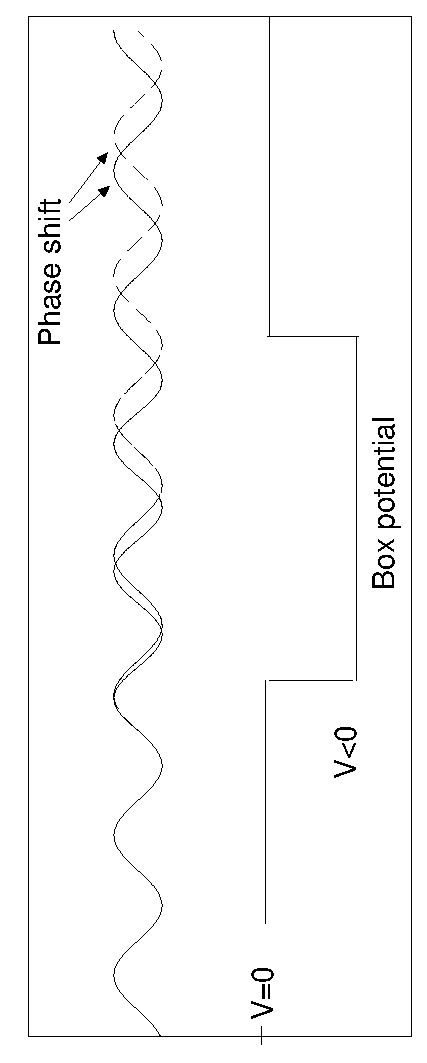
\includegraphics[height=15cm,angle=-90]{detteerfaseskift.eps}
\caption{Shows how a wave function will behave for a attractive box potential. The dashed line
illustrates the wave function behavior with out the potential.}
\end{figure}
\end{flushleft} 
However the phase shift can not be found directly. Experimentalist have to study the observable, 
which can be for example differential cross section and polarization. With these data, theorists are
able to calculate an NN-amplitude (A) for the process. This amplitude has many of the same properties as the S-matrix,
like the unitarian. In partial wave decomposition, it is related to the phase shift $\delta_l$ as
\begin{equation}
A_l=\eta_l e^{i2\delta_l}
\end{equation}

Inelasticity ($\eta_l$) is the probability amplitude for the scattering amplitude to be elastic. 
The inelasticity and phase shift are the necessary parameters to describe a partial wave. The inelasticity
becomes important for NN-scattering when the kinetic energy in the lab-system are above 350 MeV.
The inelasticity are due to energy released from the NN-system. This can be done by photon emission and/or particle
creations in the scattering.

  
%fig~\ref{fig:manypotS} shows the phase shift for different potentials and experimental phase shift.
%How the potentials are build up will be explained later.



\begin{flushleft} 

\begin{figure}\label{fig:manypotS}
\centering
\includegraphics[height=17cm]{manypotS.eps} 
\caption{\state{1}{S}{0} phase shifts for a box Potential, a parameterized potential, the Bonn B potential and
experimental data ~\cite{PRC48faseskift350MeV}. How the potentials are build up will be explained later.}
\end{figure}


\end{flushleft}


 
\kap{Scattering Theory}\label{chap:scattering}
%\begin{flushleft}

In this chapter much of the theoretical theory for the Nucleon-Nucleon (NN) scattering is derived, 
focusing on deriving practical expressions later used in the computer program. i.e. 
formulas for The S-matrix, T-matrix, phase shifts and inelasticities.
Instead of working with the exact quantum field theory, we develop an approximation from it that involves a S-matrix.
This S-matrix is analog to the familiar S-matrix in classical scattering theory.
So much of the space will be dedicated to deriving central formulas in scattering theory.
And how one derive different S-matrixes from quantum field theory.
One also have to introduce a special S matrix for coupled channels. Deuteron is a bound state of a
proton and a neutron, 
and is an example of such a case. To deal with coupled channels, one have to 
define a mixing parameter along with the phase shift.

Later will also simple potential models be derived. Potentials like the box potential and the parameterized
potential are primitive, but they give a good physical understanding of the NN interactions. The box potential
is also a good way of testing the computational methods that calculate the phase shift, 
since its theoretical phase shift is easy to calculate.
%\nl
%\nl



%Many of the equations I have used in in the computer programs are taken 
%directly from non relativistic scattering theory based on quantum mechanics.
%Therefor I feel it is natural to first derive the equations I use. Mainly focusing on 
%finding practical expressions for The S-matrix, T-matrix, phase shifts and inelasticities.
%\nl
%\nl
\section{Perturbation Theory} 

A Nucleon-Nucleon or a general multiple nucleon system is described by a Hamiltonian 
$\op{H}$ which can be divided into two parts
$\op{H}=\op{H_0}+\op{V}$. Where the dominant part is the unperturbation Hamiltonian $\op{H_0}$ whitch
contains information of each nucleon in absence of the others, and $\op{V}$ is this
interaction term between the nucleons. The time independent {\SE} can be written as
%                                                 
\begin{equation}\label{eq:timeindependentSL}
\big( \op{H_0} +\op{V} \big)\ket{\psi_{\bf k}} = E_{\bf k} \ket{\psi_{\bf k}} 
\end{equation}
%                                                 
$\ket{\psi_{\bf k}}$ can be divided into two orthogonal parts
$\ket{\psi_{\bf k}}=\ket{\phi_{\bf k}}+\ket{\chi_{\bf k}}$ . Where $\ket{\phi_{\bf k}}=\ket{{\bf k}}$
is the free part, and $\ket{\chi_{\bf k}}$ is the perturbated part.
So we have the unperturbated equation
we are familiar with
%                                                 
\begin{equation}
\op{H_0}\ket{\phi_{\bf k}}=\frac{\op{{\bf k}}^2}{2m}\ket{\phi_{\bf k}}=E_{\bf k}\ket{\phi_{\bf k}}
\end{equation} 
%                                                 
Now using the free Greens function defined as
%                                                 
\begin{equation}\label{eq:fgreen}
\op{G}^{(\pm)}_0(E)=\lim_{\epsilon \rightarrow 0} \inv{E-\op{H}_0\pm i\epsilon}
\end{equation}
%                                                 
Where $\epsilon$ is a regulator that decides if the green operator is carrying the state
forward or backwards in time.
We can now rewrite $\ket{\psi_{\bf k}}$ as an iteration equation
 %                                                 
\begin{equation}\label{eq:ket}
\ket{\psi_{\bf k}^{\pm}}=\ket{\phi_{\bf k}}+\op{G}^{(\pm)}_0(E_{\bf k})\;\op{V}\;\ket{\psi_{\bf k}^{\pm}}
\end{equation}
%                                                 
It's easy to verify that state satisfies the time independent \SE 
%                                                 
\begin{equation}
(E-\op{H}_0)\;\ket{\psi_{\bf k}^{\pm}}=\op{V}\ket{\psi_{\bf k}^{\pm}}
\end{equation} 
%                                                 
we have
%                                                 
\begin{equation} 
(E-\op{H}_0)\;\ket{\phi_{\bf k}}=0
\end{equation}
%                                                 
and
%                                                 
\begin{equation}
(E-\op{H}_0)\;\op{G}^{(\pm)}_0(E_{\bf k})\;\op{V}\;\ket{\psi_{\bf k}^{\pm}}=\op{V}
\end{equation}
%                                                 
%                                                 
So (~\ref{eq:ket}) is therefor exact.  
We use the expression "Born approximation of order n" to say how many
times we iterate this equation and where we end the last iteration with the approximation
$\ket{\psi_{\bf k}}=\ket{\bf k}$ Using that $\ket{\phi_{\bf k}}=\ket{\bf k}$
and iterate infinite times we will get
%                                                 
\begin{equation}\label{eq:G}
\ket{\psi_{\bf k}^{\pm}}=\big(1+\op{G}^{(\pm)}(E_{\bf k})\;\op{V}\big)\;\ket{\bf k}
\end{equation}
%                                                 
where
%                                                 
\begin{eqnarray}\label{eq:GG}
\op{G}^{(\pm)} &=& \op{G}^{(\pm)}_{0}+\op{G}^{(\pm)}_{0}\op{V}\op{G}^{(\pm)} \nonumber\\
&=&
\op{G}^{(\pm)}_{0}+\op{G}^{(\pm)}_{0}\op{V}\op{G}^{(\pm)}_{0}
+\op{G}^{(\pm)}_{0}\op{V}\op{G}^{(\pm)}_{0}\op{V}\op{G}^{(\pm)}_{0}+\ldots
\end{eqnarray}
%                                                 
If we now make use of the general operator relation
%                                                 
\begin{equation}
\inv{\op{A}+\op{B}}=\inv{\op{A}}+\inv{\op{A}}\op{B}\inv{\op{A}}+\inv{\op{A}}\op{B}
\inv{\op{A}}\op{B}\inv{\op{A}}+\ldots
\end{equation}
%                                                 
We see that
%                                                 
\begin{equation}
\op{G}^{(\pm)}(E)=\inv{E-\op{H}_0-\op{V}\pm i\epsilon}
\end{equation}
%                                                 
Now $\op{G}^{(\pm)}(E)$ is the Green function for the full Hamilton operator 
$\op{H}=\op{H_0}+\op{V}$ and we can write the time independent {\SE} 
(~\ref{eq:timeindependentSL}) as
%                                                 
\begin{equation}
\big(E_{\bf k}-\op{H}\big)\ket{\psi_{\bf k}^{\pm}}=0
\end{equation}
%                                                 
Where an expression of $\ket{\psi_{\bf k}^{\pm}}$ is given in (~\ref{eq:G})






\section{S- and T-matrix}
%putt inn en figur se vinkel nedenfor!!!!!!!!!!!!!!!!!!!!!!!!!!!!!!!!!!!!!!
%se Hemmer s 262




The scattering operator or also often called the  S-matrix is defined by
%                                                 
\begin{equation}
S({\bf{p}},{\bf{k}})=\braketm{\bf{p}}{\op{S}}{\bf{k}}=\braket{\psi_{\bf{p}}^{-}}{\psi_{\bf{k}}^{+}} 
\end{equation}
%                                                 
This definition tells us that $S(\op{p},\op{k})$ must be the probability
amplitude of finding a free incoming particle in state $\ket{\op{k}}$ which is an 
eigenstate of the free Hamiltonian and a free outgoing particle in state $\ket{\op{p}}$.
And $\op{p}$ is in the direction of the scattering angle $\theta$. Where $\theta$ 
is the angle between $\op{p}$ and $\op{k}$. Since $\op{V}$ 
and$\op{H}_0$ are operators of observables they must be Hermitian. That is $\op{V}=\op{V}^\dagger$ and
$\op{H}_{0}=\op{H}^{\dagger}_{0}$. From this follows
%                                                 
\begin{equation}
(\op{G}^{(\pm)})^\dagger=\op{G}^{(\mp)}
\end{equation}
%                                                 
We  see that  by taking the Hermitian adjunct on both sides of $(~\ref{eq:G})$ 
we get
%                                                 
\begin{equation}\label{eq:Gdagger}
\bra{\psi_{\bf k}^{\pm}}=\bra{\op k}\big(1+\op{V}\;\op{G}^{(\mp)}(E_{\bf k})\big)
\end{equation}
%                                                 
From definition should $\braket{\psi_{\bf{p}}^{+}}{\psi_{\bf{k}}^{+}}$ have
the same probability amplitude as $\braket{\bf{p}}{\bf{k}}$. That is
%                                                 
\begin{equation}
\braket{\psi_{\bf{p}}^{+}}{\psi_{\bf{k}}^{+}}=\braket{\bf{p}}{\bf{k}}
\end{equation}
%                                                 
We now use a little trick where we add zero. 
%                                                 
\begin{eqnarray}
\braket{\psi_{\bf{p}}^{-}}{\psi_{\bf{k}}^{+}} &=&
\braket{\psi_{\bf{p}}^{+}}{\psi_{\bf{k}}^{+}}+\big(\bra{\psi_{\bf{p}}^{-}}
-\bra{\psi_{\bf{p}}^{+}}\big)\ket{\psi_{\bf{k}}^{+}}\nonumber\\
&=&
\braket{{\bf{p}}}{{\bf{k}}}+\bigg( \inv{E_{\bf{p}}-E_{\bf{k}}+i\epsilon}-
\inv{E_{\bf{p}}-E_{\bf{k}}-i\epsilon}\bigg) \braketm{\bf{p}}{\op{V}}{\psi_{{\bf k}}^{+}}
\end{eqnarray}
%                                                 
If we use the relations
%                                                 
\begin{eqnarray}\label{eq:P1}
\inv{x+i\epsilon}={\cal P} \inv{x}-i\pi\delta (x)\\\label{eq:P2} 
\inv{x-i\epsilon}={\cal P} \inv{x}+i\pi\delta (x)
\end{eqnarray} 
%                                                 
Where ${\cal P}$ is Cauchy's principal value. Using these equations we have a well-known expression for the S-matrix
%                                                 
\begin{equation}\label{eq:Sgenerel} 
S({\bf{p}},{\bf{k}})=
\braket{\psi_{\bf{p}}^{(-)}}{\psi_{\bf{k}}^{(+)}}=\braket{{\bf{p}}}{{\bf{k}}}
-2\pi i \delta (E_{\bf p}-E_{\bf k})
\braketm{{\bf p}}{\op{T}}{\bf{k}}
\end{equation}
%                                                 
Or on a more abstract form the S operator can be written as:
%                                                 
\begin{equation}\label{eq:Smat} 
\op{S}=\op{1}-2\pi i \delta (\op{H}_0-E){\op{T}}
\end{equation}
%                                                 
Where we have introduced the transition operator $\op{T}$ which is defined
%                                                 
\begin{equation}\label{eq:Tdef}
\op{V}\ket{\psi_{\bf k}^{(+)}}=\op{T}\ket{{\bf k}}
\end{equation}
%                                                 
From (\ref{eq:ket}) and (\ref{eq:GG}) we see that $\op{T}$ also can be written as:
%                                                 
\begin{equation}\label{eq:TM} 
\op{T}=\op{V}+\op{V}\op{G}^{(+)}\op{V}=\op{V}+\op{V}\op{G}^{(+)}_0\op{T} 
\end{equation}
%                                                 
This is the $\LS$ equation on a general operator form.
A useful feature of the S-matrix when programming is the unitarity of the S-matrix when the potential is real.
Which means that we have elastic scattering.
In such a scattering we must therefore have $SS^{\dagger}=\op{1}$. This is easy to check in the program.
If $SS^{\dagger}\ne \op{1}$ then something is wrong in the program. We can prove this unitarity
by shoving  that $\braketm{{\bf p}}{\op{S}\op{S}^{\dagger}}{{\bf k}}=
\braket{{\bf p}}{{\bf k}}$. We note that
%                                                 
\begin{eqnarray}
\op{S}\ket{{\bf k}}=\ket{{\bf k}}-2\pi i \delta (H_0-E_{\bf k}){\op{T}}\ket{{\bf k}}\\
\bra{{\bf p}}\op{S}^{\dagger}=\bra{{\bf p}}
+\bra{{\bf p}}{\op{T}}^{\dagger}  2\pi i \delta (H_0-E_{\bf p}) 
\end{eqnarray}
%                                                 
Putting these two equations together we have
%                                                 
\begin{eqnarray}\label{eq:Uni} 
\braketm{{\bf p}}{\op{S}^{\dagger}\op{S}}{{\bf k}} &=&
\braket{{\bf p}}{{\bf k}}-2\pi i \delta (E_{\bf k}-E_{\bf p})\braketm{{\bf p}}
{(\op{T}-\op{T}^{\dagger})}{{\bf k}}\nonumber\\
& &
-(2\pi i)^2 
\braketm{{\bf p}}{\op{T}^{\dagger}\delta (E_{\bf k}-H_0 ) \delta (E_{\bf p}-H_0 )
\op{T}}{{\bf k}}
\end{eqnarray}
%                                                 
So we have to show that term 2 and 3 on the right-hand side of (\ref{eq:Uni}) cancel 
each other. From (\ref{eq:TM}) we have $\op{T}=\op{V}+\op{V}\op{G}^{(+)}_0\op{T}$. 
From this we get the relation
%                                                 
\begin{equation}\label{eq:TMC} 
\op{T}^{\dagger}=\op{V}+\op{T}^{\dagger}\op{G}^{(-)}_0\op{V}
\end{equation}
%                                                 
If we use (\ref{eq:TM}) in (\ref{eq:TMC})  we get
%                                                 
\begin{equation}\label{eq:TMCT}
\op{T}^{\dagger}=\op{V}+\op{T}^{\dagger}\op{G}^{(-)}_0\op{T}-\op{T}^{\dagger}
\op{G}^{(-)}_0\op{V}\op{G}^{(+)}_0\op{T}
\end{equation}
%
Do the same with (\ref{eq:TM}). That is, substitute the last $V$ in (\ref{eq:TM}) with
%
\begin{equation}
\op{V}=\op{T}^{\dagger}-\op{V}\op{G}^{(+)}_0\op{T}
\end{equation}
%
and
%
\begin{eqnarray}\label{eq:bevisT}
\op{T}^{\dagger}-\op{T} &=& \op{V}+\op{T}^{\dagger}\op{G}^{(-)}_0\op{T}-\op{T}^{\dagger}
\op{G}^{(-)}_0\op{V}\op{G}^{(+)}_0\op{T}\nonumber\\
& &
-\big[\op{V}+\op{T}^{\dagger}\op{G}^{(+)}_0\op{T}-\op{T}^{\dagger}
\op{G}^{(-)}_0\op{V}\op{G}^{(+)}_0\op{T}\big]\nonumber\\
&=&
\op{T}^{\dagger}\op{G}^{(-)}_0\op{T}-\op{T}^{\dagger}\op{G}^{(+)}_0\op{T}\nonumber\\ 
&=&
\op{T}^{\dagger}\big[\op{G}^{(-)}_0-\op{G}^{(+)}_0\big]\op{T}\nonumber\\
&=&
\op{T}^{\dagger}\bigg[\inv{E-\op{H}_0-i\epsilon}-
\inv{E-\op{H}_0+i\epsilon}\bigg]\op{T}\nonumber\\ 
&=& 
2\pi i \op{T}^{\dagger} \delta (E-\op{H}_0 )\op{T}
\end{eqnarray}
%                                                 
Where $E$ is either $E_{\bf k}$ or $E_{\bf p}$ and we have used (\ref{eq:P1}) and (\ref{eq:P2}) in the last step 
. Noting that
%
\begin{equation}
\delta (E_{\bf k}-H_0 ) \delta (E_{\bf p}-H_0 ) = 
\delta (E_{\bf k}-E_{\bf p} ) \delta (E-H_0 ) 
\end{equation}
%
Finally the 2. and 3. terms on the right-hand side of (\ref{eq:Uni}) will
cancel each other. And therefor the S-matrix must be unitary in this case.
\newline
\newline
In the case of the scattering process we have ($E>0$).

When we want to insert a complete set of
eigenstates in the Green function, we only include the states with positive $E$. i.e.
we remove the bound states from the complete set of eigen states. We are then  
left with the continuous specter of momentum as a basis.
This will be a  projection of (\ref{eq:TM}) into momentum space. 
It's convenient to work in momentum space since 
we then have an integral equation instead of a differential equation when solving it in coordinate space 
(The $\SE$ equation). 
%The interaction potential $V$
%is dependent on the relative 
%distance between the particles. By doing a transformation of $V$ into momentum space, which is
%a Fourier transformation. 
%We have a local potential that is only dependent upon the relative velocities.
If we now use the ket relation found in (\ref{eq:ket}) with the definition of T (\ref{eq:Tdef}), we have 
%
\begin{eqnarray}  
\ket{\psi_{\bf k}^{+}} &=& \ket{{\bf k}}+\op{G}^{(+}_0(E_{\bf k})\;\op{V}\;
\ket{\psi_{\bf k}^{+}} \nonumber\\ 
&=&
\ket{{\bf k}}+ \inv{E_{\bf k}-\op{H}_0+i\epsilon}   \;\op{T}\;
\ket{{\bf k}}\nonumber\\
&=&
\ket{{\bf k}}+ \inv{(2\pi)^3}\int^{\infty}_{\infty}d^3 {\bf q}\quad \ket{{\bf q}}\bra{{\bf q}}
\inv{E_{\bf k}-E_{\bf q}+i\epsilon}   \;\op{T}\;\ket{{\bf k}}
\end{eqnarray}  
%
Where we in the last step inserted a complete set of positive energy states.
By multiplying this equation with $\bra{{\bf p}}\op{V}$ from the left, we get 
%
\begin{equation}\label{eq:Tmatp}
\braketm{{\bf p}} {\op{T}(E)}{{\bf k}} =\braketm{{\bf p}}{\op{V}}{{\bf k}}
+ \inv{(2\pi)^3}\int^{\infty}_{\infty}d^3 { q} \quad\bra{{\bf p}}\op{V}\ket{{\bf q}}\bra{{\bf q}}
\inv{E_{\bf k}-E_{\bf q}+i\epsilon}   \;\op{T}(E)\;\ket{{\bf k}}
\end{equation}
%
Where $E$ is the on-shell energy.

This $\LS$ equation has almost the same form as the one I use in my computer program.
To get the form which 
I use, one has to do a partial wave decomposition of (\ref{eq:Tmatp}). 
This can be practical if the potential is central/local, i.e.        %SJEKK DETTE
$V({\bf r}_1{\bf r}_2)=V({\bf r})$. So that $\Delta\times V({\bf r})=0$.
We are then able to reduce the two particle problem to a one particle problem by
working in the mass center system, where we use the particles relative coordinates ({\bf r}). 
%The transformation from lab- too MC-system of the $\SE$,
%is done later in this chapter.
A local potential has therefor spherical symmetry
with respect to the two particles relative coordinates ${\bf r}$.
This way we have reduced the three-body force to a familiar two-body force.
We can make such a potential by using
meson theory if we assume single wave channel as a good approximation. For example the 
One Boson Exchange model (OBE) is based upon this approximation, which is done by approximating all
higher wave channels by a fictive/effective $\sigma$ meson.

%For a general local potential $V=V(r)$ we can transform it to 
%momentum space by doing a Fourier transform.

We note that $\exp (i{\bf kr})$ can be written in terms of Legendre polynomials 
$P_l({\bf \op{k}\op{r}})$ and spherical Bessel functions $j_l ({ kr})$. Which is known as the 
Bauer series
%%%%%%%%%%%%%%%DEF se side 9 i morten not!!!!!!!!!!!!!!!!!!!!!!!!!!!!!!!!!!!!!!!!!!!!!!!!!!!!!!!!!!!!!!!!!!!!!!!!!!!!!!!!!!!!!!!!!!!!!!!!!!!!!!!!!!!!!!!!!!!
%
\begin{equation}
\exp (i{\bf kr})=\sum^{\infty}_{l=0} (2l+1) i^{l} j_{l}(kr)P_l({\bf \op{k}\op{r}})
\end{equation}

Where the angular momentum quantum number $l$ has been introduced. We then have
for a local potential
%
\begin{flushleft} 
\begin{eqnarray}
&&\langle{{\bf p}}|{\op{V}}\ket{{\bf k}} =\int^{\infty}_{-\infty}d^3r
\exp (-i{\bf pr})V({\bf r})\exp (i{\bf kr})\nonumber\\
&=&
\int^{\infty}_{-\infty}d^3r
\sum^{\infty}_{l'=0} (2l'+1) i^{-l'} j_{l'}(pr)P_{l'}({\bf \op{p}\op{r}}) V({\bf r})
\sum^{\infty}_{l=0} (2l+1) i^{l} j_{l}(kr)P_l({\bf \op{k}\op{r}})\nonumber\\ 
&=&
2\pi\sum^{\infty}_{l,l'=0}(2l'+1)(2l+1) i^{(l-l')}
\int^{\infty}_{0}dr\;r^2 V(r) j_{l'}(pr)j_{l}(kr) \int^{1}_{-1}d({\cos \theta}) 
P_{l'}({\bf \op{p}\op{r}})P_l({\bf \op{k}\op{r}})\nonumber\\
&=&
4\pi\sum^{\infty}_{l=0} (2l+1) P_{l}({\bf \op{p}\op{k}})
\int^{\infty}_{0}dr\;r^2 V(r) j_{l}(pr)j_{l}(kr) 
\end{eqnarray}
\end{flushleft} 
%
Where the z-axis is taken to be in the direction of the incoming particle (${\bf \op{p}}$).
This is done because we expect to see axial symmetry around the z-axis from the scattering. So 
that ${\bf \op{p}\op{k}}$ denote the angle between ${\bf \op{p}}$ and ${\bf \op{k}}$.
In the last step we used the Legendre polynomial relation

\begin{equation}\label{eq:poly}  
 \int^{1}_{-1}d\big({\cos({\bf \op{p}\op{k}})}\big)P_{l'}({\bf \op{p}\op{r}})P_l({\bf \op{k}\op{r}})
 =\frac{2}{2l+1}\;P_{l}({\bf \op{p}\op{k}})\;\delta_{l,l'}
\end{equation}
%
We then define
%
\begin{equation}\label{eq:V_l_def}
V_l({ p},{ k})=\braketm{{ p}}{{\op{V}}_l}{{ k}}=
\int^{\infty}_{0}dr\;r^2 V(r) j_{l}(pr)j_{l}(kr) 
\end{equation}
%
So we have
%
\begin{equation}
V({\bf p},{\bf k})=
4\pi\sum^{\infty}_{l=0} (2l+1) P_{l}({\bf \op{p}\op{k}}) V_l({ p},{ k})
\end{equation}
%
From the definition of $\op{T}$ we have $\op{V}\ket{\psi_{\bf k}^{(+)}}=\op{T}\ket{{\bf k}} $
. We define $\op{T}_l$ so that it satisfies a similar equation
$\op{V}_l\ket{\psi_{ k}^{(+)}}=\op{T}_l\ket{{ k}} $\; , and we have
%
\begin{equation}\label{eq:TsomTm} 
\braketm{{\bf p}}{T}{{\bf k}}=
4\pi\sum^{\infty}_{l=0} (2l+1) P_{l}({\bf \op{p}\op{k}}) \braketm{{ p}}{T}{{ k}}
\end{equation}
%
By using these relations we have
%
\begin{eqnarray} 
&&\inv{(2\pi)^3}\int^{\infty}_{-\infty}d^3 { q} \quad\bra{{\bf p}}\op{V}\ket{{\bf q}}\bra{{\bf q}} 
\inv{E-E_{\bf q}+i\epsilon}   \;\op{T}(E)\;\ket{{\bf k}} 
\nonumber\\  
&=&
\frac{2}{\pi}\sum^{\infty}_{l,l'=0}\int^{\infty}_{-\infty}d^3 { q}
(2l+1)P_l({{\bf p}}{{\bf q}})V_{l}(p,q)
\inv{E-E_{\bf q}+i\epsilon}
(2l'+1) P_{l'}({\bf \op{q}\op{p}})\bra{q}\op{T}_{l'}(E)\ket{{ k}}\nonumber\\
&=&
%\frac{64\pi^3}{(2\pi)^3}
8\sum^{\infty}_{l=0}(2l+1) P_{l}({\bf \op{p}\op{k}})
\int^{\infty}_{0}dq\quad
V_{l}(p,q)\inv{E-E_{\bf q}+i\epsilon}
\bra{q}\op{T}_{l}(E)\;\ket{{ k}}
\end{eqnarray}
%
We have now a  partial wave expression for all the terms in the $\LS$ (\ref{eq:Tmatp}) equation.
%If we now choose to work in the mass center
, and we can rewrite it as
%
%\begin{eqnarray}
%&&\braketm{{\bf p}} {\sum^{\infty}_{l=0} (2l+1) P_{l'}({\bf \op{p}\op{k}})\op{T}_l(E)}{{\bf k}} =
%\sum^{\infty}_{l=0} (2l+1) P_l({\bf \op{p}\op{k}}) \braketm{{\bf p}}{\op{V}_l}{{\bf k}}\nonumber\\
%&&
%+
%\frac{4\pi^2}{(2\pi)^3}\sum^{\infty}_{l,l'=0}\int^{\infty}_{\infty}d {\bf q} 
%(2l+1)P_l({{\bf p}}{{\bf q}})V_{l}(p,q)
%\inv{E-E_{\bf q}+i\epsilon} 
%(2l'+1) P_{l'}({\bf \op{q}\op{p}})\op{T}_{l'}(E)\;\ket{{\bf k}}\nonumber\\ 
%\end{eqnarray}
%By using (\ref{eq:poly}) again we get
%
\begin{equation}\label{eq:Tmy}
\braketm{{ p}} {\op{T}_l(E)}{{ k}} =\braketm{{ p}}{\op{V}_l}{{ k}}
+ \frac{2}{\pi}\int^{\infty}_{0}d { q}\; q^2 \quad\bra{{ p}}\op{V}_l\ket{{ q}}
\inv{2E-2E_{\bf q}+i\epsilon}  \bra{{ q}} \;\op{T}_l(E)\;\ket{{ k}}
\end{equation}
From (\ref{eq:P1}) and (\ref{eq:P2}) we have
\begin{equation}\label{eq:Tmyekstra}
\inv{2E_{\bf k}-2E_{\bf q}\pm i\epsilon}={\cal P}\inv{2E_{\bf k}-2E_{\bf q}}\mp 
i\pi\delta(2E_{\bf k}-2E_{\bf q})={\cal P}\inv{2E_{\bf k}-2E_{\bf q}}\mp 
\frac{i\pi\delta({ k}-{ q})}{2\big|\frac{\partial E_{\bf q}}{\partial { q}}\big|_{{ k}}}
\end{equation}
Where we have in the last step used the general formula for the delta function.
\begin{equation}\label{eq:deltaf} 
\delta (f(x))=\inv{\big|\frac{\partial f(x)}{\partial x}\big|_{x_0}}\delta (x_0)
\end{equation}
%
%The final expression will depend on if we use relativistic energies or not in the propagator. 
%The relativistic form of $\op{T}$ has to be derived from relativistic scattering theory. 
%For relativistic energies $E_{\bf q}=\sqrt{{\bf q}^2+m^2}$ we have
%\begin{equation}\label{eq:Trel}  
%\bigg|\frac{\partial E_{\bf q}}{\partial {\bf q}}\bigg|_{{\bf k}}=\frac{{\bf k}}{\sqrt{{\bf k}^2+m^2}}
%\end{equation} 
%
For $E_{\bf q}=\frac{{ q}^2}{2m}$ we get
%
\begin{equation}\label{eq:Tnrel}
\bigg|\frac{\partial E_{\bf q}}{\partial { q}}\bigg|_{{ k}}=\frac{{ k}}{m}
\end{equation}
%
So the $\LS$ equation can be written as
%
\begin{eqnarray}\label{eq:Tnrelllll} 
\braketm{{ p}} {\op{T}_l(E_{ k})}{{ k}}&=&\braketm{{ p}}{\op{V}_l}{{ k}}
+ \frac{2m}{\pi}\;{\cal P}\int^{\infty}_{0}d { q}\; q^2 \quad\bra{{ p}}\op{V}_l\ket{{ q}}
\;\inv{{ k^2}-{ q^2}}   \;\bra{{ q}}\op{T}_l(E_{ k})\ket{{ k}}\nonumber\\
&&
-i { k}m \;\bra{{ p}}\op{V_l}\ket{{ k}}
   \;\bra{{ k}}\op{T}_l(E_{ k})\;\ket{{ k}}
\end{eqnarray}
%
Now when we have an expression for $\op{T}_l$ we would like to use it to calculate the phase shifts
and the inelasticities, which are the experimental values we can obtain from such a scattering process.
It turns out that they are very close related to the $\op{S}_l$, which will soon be explained.
If we have an elastic scattering, then $\op{S}$ is unitary as proved earlier in this chapter.
We then have
%
\begin{equation}\label{eq:Slun}
\braketm{{\bf p}}{\op{S}^\dagger \op{S}}{{\bf k}}=\int^{\infty}_{-\infty} d^3 { r}\;
\braketm{{\bf p}}{\op{S}^\dagger }{{\bf r}}\braketm{{\bf r}}{\op{S} }{{\bf k}} 
=\braketm{{\bf p}} {\;\op{1}\;}{{\bf k}}=(2\pi)^3\;\delta ({\bf p}-{\bf k})
\end{equation}
%
We also want to rewrite $\braketm{{\bf r}}{\op{S} }{{\bf k}}$ as a partial
wave expansion
%
\begin{eqnarray}\label{eq:Slutledning}  
\braketm{{\bf r}}{\op{S} }{{\bf k}} 
&=&
\int^{\infty}_{-\infty} \frac{d^3 { q}}{(2\pi)^3}\;\braket{{\bf r}}{{\bf q}}
\braketm{{\bf q}}{\op{S} }{{\bf k}}\nonumber\\
&=&
\int^{\infty}_{-\infty} \frac{d^3 { q}}{(2\pi)^3}\; \exp(i{\bf rp})\big(\;
\braket{{\bf q}}{{\bf k}} -2\pi i\; \delta (2E_{\bf q}-2E_{\bf k})\;\braketm{{\bf q}}{\op{T}}{\bf{k}}\;\big)\nonumber\\  
&=&
\exp(i{\bf rk})-\bigg[ i^{l+1}m\int^{\infty}_{0}dq\;q\;\delta (q-k)\nonumber\\
&&\qquad 
\sum^{\infty}_{l,l'=0}j_{l}(kr)(2l+1)(2l'+1)\;\bra{q}\op{T}_{l}\;\ket{{ k}}\;\int^{1}_{-1}d(\cos\theta)\; P_{l'}
({\bf \op{q}\op{k}})P_{l}({\bf \op{q}\op{r}})\bigg] \nonumber\\
&=& 
\sum^{\infty}_{l=0} (2l+1) i^{l} j_{l}(kr)P_l({\bf \op{k}\op{r}})\big[1-2imk\;\bra{k}\op{T}_{l}\;\ket{{ k}} \big]
\end{eqnarray}
%
Where we have used (\ref{eq:deltaf}) and (\ref{eq:Tnrel}) to rewrite $\delta (2E_{\bf q}-2E_{\bf k})$ for 
$E_{\bf k}=\frac{{\bf k}^2}{2m}$. We define ${\op{S} }_l$ to be
%
\begin{equation}\label{eq:Sl} 
\op{S}_{l}\ =1-2imk\;\bra{k}\op{T}_{l}\;\ket{{ k}}
\end{equation}
%
So that
%
\begin{equation}\label{eq:SSl}
\braketm{{\bf r}}{\op{S} }{{\bf k}} =\sum^{\infty}_{l=0} (2l+1) i^{l} j_{l}(kr)P_l({\bf \op{k}\op{r}})\;\op{S}_{l}
\end{equation}
%
Now we can show that also ${\op{S} }_l$ is unitary if we have an elastic scattering. By
using (\ref{eq:Slun}), (\ref{eq:SSl}) and choosing $|\op{S}_{l}|=1$ for all $l$
%
\begin{equation}\label{eq:SSlun}
\int^{\infty}_{-\infty} d^3 { r}\;
\braketm{{\bf p}}{\op{S}^\dagger }{{\bf r}}\braketm{{\bf r}}{\op{S} }{{\bf k}}
=
\int^{\infty}_{-\infty} d^3 { r}\; \exp(i{\bf r(k-p)})=(2\pi)^3\delta ({\bf p}-{\bf k})
\end{equation}
%
We see that $|\op{S}_{l}|=1$ gives the right result.
\nl
For inelastic scattering we have a complex potential which
makes creation of other particles possible. In this process energies are taken from the nucleons, or even excited
to other barions. 
Since this will reduce the velocity of the nucleons, we also get a reduced flux out after the scattering.
So we always have $|\op{S}_{l}|\le 1$ in a scattering process. The creations of other particles have to
follow certain rules such as the nucleon number, total spin, isospin, momentum, energy and charge are 
conserved in the process. These matters will be discussed later since we need quantum field theory to 
explain creations of new particles. 





\section[Phase shifts and Inelasticities]{The Scattering Amplitude, Phase shifts and Inelasticities}  
%figur!!!!!!!!!!!!!!!!!!!!!!!!!!!!!!!!!!!!!!!!!!!!!!!!!!!!!!
%hemmer s 262
%
The scattering process we now look at, is the situation where a particle is scattered from a
local, stationary potential $V({\bf r})$, which is the same situation we have in the mass center system
if two particles are interacting through a local/central potential.
We can use the time independent $\SE$ 
(\ref{eq:timeindependentSL}) to solve the scattering caused by the potential. 
%If we have a local potential, 
Using $E=\frac{k^2}{m}$ we can write the  $\SE$ as
%
\begin{equation}\label{eq:Slfi} 
({\bf \triangledown}^2+k^2 )\psi ({\bf r})= 2m\; V({\bf r})\;\psi ({\bf r})
\end{equation}
%
Where $\psi ({\bf r}) = \braket{{\bf r}}{\psi}$ is the wave function. The behavior of the wave function
will be very complicated near the scattering center. Further away from this center the potential grows weaker, 
and for large $r$ it can be neglected. And we will have free particle solutions from the $\SE$ equation.
Where the incoming particle is a plane wave and the outgoing/scattered particle is a radial wave.
%
\begin{equation}
\psi ({\bf r})=\psi_{in} ({\bf r})+\psi_{out} ({\bf r})\qquad {\text for}\quad r\to\infty
\end{equation}
And
\begin{equation}
\psi_{in} ({\bf r})=\exp (i{\bf kr})
\end{equation}
For an elastic scattering the kinetic energy is conserved, so the scattered wave must have the same 
wave number $k=|{\bf k}|$ as the incoming wave.
\begin{equation}
\psi_{out} ({\bf r})=f(\theta ,\varphi)\frac{\exp (i{ kr})}{r}
\end{equation}
%
$f(\theta ,\varphi)$ describes the distribution in the different directions and is called
the scattering amplitude. 
So for large $r$ we have
%
\begin{equation}\label{eq:spredamp} 
\psi ({\bf r})=\exp (i{\bf kr}) + f(\theta ,\varphi)\frac{\exp (i{ kr})}{r} 
\end{equation}
%
From (\ref{eq:ket}) we have
%
\begin{equation}\label{eq:ledd}
\braket{{\bf r}}{\psi_{\bf k}^{+}}=\braket{{\bf r}}{{\bf k}}+
\int^{\infty}_{-\infty}d^3 {{ r}'}\;\braketm{{\bf r}}{\op{G}^{(+)}_0(E_{\bf k})}{{\bf r}'}\;
{V}({{\bf r}'})\;\braket{{\bf r}'}{\psi_{\bf k}^{+}} 
\end{equation}
%
Where we need to know the Green function with respect to coordinate space. We have
%
\begin{eqnarray}
\braketm{{\bf r}}{\op{G}^{(+)}_0}{{\bf r}'} 
&=&
\int^{\infty}_{-\infty}\frac{d^3 {{ q}}}{(2\pi)^3}\;
\braketm{{\bf r}}{\inv{E-\op{H}_0+ i\epsilon} }{{\bf q}}\;\braket{{\bf q}}{{\bf r}'} \nonumber\\ 
&=&
\frac{4\pi m}{(2\pi)^3}\;\int^{\infty}_{0}dq\;q^2\int^{\pi}_{0}d\theta\; 
\frac{\sin\theta}{{{ k}^2}-{{ q}^2}+ i\epsilon}\;\exp(iq|{\bf r}-{\bf r}'|\cos\theta) \nonumber\\ 
&=& 
\frac{4\pi m}{(2\pi)^3i|{\bf r}-{\bf r}'|}\;\int^{\infty}_{0}dq\;q\;
\frac{1}{{{ k}^2}-{{ q}^2}+ i\epsilon}\;\bigg[\exp(iqr)-\exp(-iq|{\bf r}-{\bf r}'|)\bigg] \nonumber\\
&=&
\frac{4\pi m}{(2\pi)^3i|{\bf r}-{\bf r}'|}\;\int^{\infty}_{-\infty}dq\;q\;
\frac{1}{{{ k}^2}-{{ q}^2}+ i\epsilon}\;\exp(iq|{\bf r}-{\bf r}'|) \nonumber\\
&=&
-\frac{m}{2\pi |{\bf r}-{\bf r}'|}\exp(ik|{\bf r}-{\bf r}'|)
\end{eqnarray}
%
Where we used that the Green function has a simple pole in $q=+\sqrt{2mE}=k$.  
For $r\gg r'$ we have
\begin{equation} 
|{\bf r}-{\bf r}'|= r
\end{equation}  
\begin{equation} 
k|{\bf r}-{\bf r}'|=k\sqrt{r^2-2{\bf r}{{\bf r}'}+{r'}^2}=kr-\frac{{\bf r}
\cdot{{\bf r}'}}{r}+{\cal O}(\frac{1}{r})
\end{equation}  
%
Going back to (\ref{eq:ledd}) we now get
%
\begin{equation}
\braket{{\bf r}}{\psi_{\bf k}^{+}} \simeq\exp (i{\bf kr}) - \frac{\exp (i{ kr})}{r}\;\frac{m}{2\pi}
\int^{\infty}_{-\infty}d^3 {{ r}'}\;\exp \bigg(-ik\frac{{\bf r\cdot r}'}{r}\bigg)
{V}({{\bf r}'})\;\braket{{\bf r}'}{\psi_{\bf k}^{+}}
\end{equation} 
%
Comparing this with (\ref{eq:spredamp}) we see that the scattering amplitude can be written as
%
\begin{equation}\label{eq:fogT}
f(\theta ,\varphi)=-\frac{m}{2\pi}
\int^{\infty}_{-\infty}d^3 {{ r}'}\;\exp \bigg(-ik\frac{{\bf r\cdot r}'}{r}\bigg)
{V}({{\bf r}'})\;\braket{{\bf r}'}{\psi_{\bf k}^{+}}
\end{equation}
%
or
%
\begin{eqnarray}\label{eq:fogT2} 
f(\theta ,\varphi)
&=&
-\frac{m}{2\pi}
\int^{\infty}_{-\infty}\frac{d^3}{(2\pi)^3{ q}}\int^{\infty}_{-\infty}d^3 {{ r}'}\;
\exp \bigg(i{\bf qr}'-ik\frac{{\bf r\cdot r}'}{r}\bigg)
\braketm{{\bf q}}{\op{V}}{\psi_{\bf k}^{+}}\nonumber\\
&=&
-\frac{m}{2\pi}\braketm{k{\bf \op{r}}}{\op{T}}{{\bf k}}
\end{eqnarray}
%
%
%
%
If we have a local potential we can write the wave function as
%
\begin{equation}
\psi ({\bf r},\theta ,\varphi)=\sum^\infty_{l=0}\sum^l_{m=-l}c_{lm}R_l(r)Y_{lm}(\theta ,\varphi) 
\end{equation}
%
Where the $Y_{lm}$ are spherical harmonics,$c_{lm}$ are constants and 
$R_l(r)$ are radial functions satisfying the radial part of the $\SE$ 
%
\begin{equation}
\frac{d^2}{r^2}(rR_l)+\bigg[ k^2-2mV({\bf r})-\frac{l(l+1)}{r^2}\bigg](rR_l)=0
\end{equation}
%
If the z-axis is taken in the direction of the incoming particles, we get axial symmetry when $m=0$. The
spherical harmonics $Y_{lm}(\theta ,\varphi)\propto P_l^{|m|}\cos\theta e^{im\phi}$ can then be written as
Legendre polynomials
$Y_{lm}(\theta)\propto P_l(\cos\theta)$ and the wave function will be
%
\begin{equation}
\psi ({\bf r},\theta)=\sum^\infty_{l=0}C_l R_l(r)P_{l}(\cos\theta )
\end{equation}
%
$C_l$ are constants. So let us find this partial wave expression of $\psi (r)$. Using the $\SE$ equation
given in (\ref{eq:Slfi}) and look at large  $r$ where the potential can be neglected if
$V(r)\propto 1/r^n$, and $n\gg 1$. We have  
%
\begin{equation}
({\bf \triangledown}^2+k^2 )\psi ({\bf r})=0\qquad {\text for}\quad r\to \infty 
\end{equation}
%
This equation has the general solution
%
\begin{equation}
\psi ({\bf r})=c_l e^{\pm i({\bf kr}+\delta_l)}
\end{equation}
%
Two constants are used to generate the general this solution. $\delta_l$ which is known as the phase shift of
the partial wave with angular momentum $l$, and $c_l$ witch is an arbitrary constant. Since this is a scattering 
process, only the outgoing wave has a physical meaning.
Writing the $e^{ i({\bf kr}+\delta_l)}$ in terms of partial waves
%
\begin{equation}
\psi ({\bf r})\bigg|_{r\to \infty}=c_l\sum^\infty_{l=0}(2l+1)\;i^l j_l({ kr}+\delta_l)\; P_l(\cos\theta)
\end{equation}
%
In the asymptotic region where $r\to \infty$ we can write the spherical Bessel function $j_l(kr+\delta_l)$ as
%
\begin{eqnarray}
j_l(kr+\delta_l)\bigg|_{r\to \infty}
&=&
\inv{kr}\sin\big(kr+\frac{\pi}{2}l+\delta_l\big)\nonumber\\
&=& 
\inv{2ikr}\bigg[e^{i(kr+\frac{\pi}{2}l+\delta_l)}-e^{-i(kr+\frac{\pi}{2}l+\delta_l)}\bigg]
\end{eqnarray}
%
If we then subtract the incoming wave from the total wave function
%
\begin{equation}
\psi ({\bf r})\bigg|_{r\to \infty}-e^{i{ kr}}=\sum^\infty_{l=0}\frac{2l+1}{2ikr}i^l 
\bigg[(c_l e^{ i({ kr}+\delta_l)}-1) e^{ i{ kr}}-(c_l e^{ i({ kr}+\delta_l)}-1) e^{-i{ kr}}\bigg]P_{l}(\cos\theta ) 
\end{equation}
%
This equation contains both incoming and outgoing spherical wave terms for large $r$.
By choosing $c_l=e^{ i\delta_l}$ we can remove the incoming spherical wave
%
\begin{equation}
\psi ({\bf r})\bigg|_{r\to \infty}-e^{i{ kr}}=\frac{e^{ i({\bf kr}}}{2ikr}\sum^\infty_{l=0}(2l+1)\;i^l
\big(e^{ i({\bf kr}+2\delta_l)}-1\big)\;P_{l}(\cos\theta )  
\end{equation}
%
From the definition of the scattering amplitude (\ref{eq:spredamp} ) we obtain $f(\theta)$
which is no longer dependent on $\varphi$ because of the symmetry around the z-axis
%
\begin{equation}\label{eq:fpart}
f(\theta)=\inv{2ik}\sum^{\infty}_{l=0} (2l+1)(e^{2i\delta_l}-1) P_{l}(\cos\theta)
\end{equation} 
%
Or alternatively by using $e^{2i\delta_l}-1=2ie^{i\delta_l}\sin\delta_l$
%
\begin{equation}
f(\theta)=\inv{k}\sum^{\infty}_{l=0} (2l+1)e^{i\delta_l}\;\sin\delta_l\; P_{l}(\cos\theta)
\end{equation}
%
This is the partial wave expansion of the scattering amplitude.


Inserting the expression of $\braketm{{ p}}{T}{{ k}}$ we have from  (\ref{eq:TsomTm}) and 
(\ref{eq:fpart}) for $f(\varphi)$ we get $T_l$ as a function of the partial wave phase shifts
%
\begin{equation}\label{eq:TsomTme} 
\braketm{{ p}}{T}{{ k}}=\inv{2mik}\bigg[1-e^{2i\delta_l}\bigg]
\end{equation}
%
Using this $T_l$ in (\ref{eq:Sl}) we get
%
\begin{equation}\label{eq:deltask}
S_l=e^{2i\delta_l}
\end{equation}
%
%If we have an inelastic scattering, 
We want to define $S_l$ for inelastic scattering, 
in such a way that we can still use methods developed for phase shifts in elastic scattering.
%
%
\begin{equation}\label{eq:deltaski}
S_l=\eta_l\; e^{2i\delta_l}
\end{equation}
%
$\eta_l$ is called the inelasticity, and we will always have $\eta_l\le 1$.
From the definitions, both $\eta_l$ and $\delta_l$ are always real. 
We note that $ e^{2i\delta_l}e^{-2i\delta_l}=1$ which is the same properties as 
$S_l$ has in an elastic scattering, and $\delta_l$ can be found the same way as before! 
\nl
The physical meaning of the inelasticity $\eta_l$, can be explained from the elastic process
\begin{equation}\label{eq:probforelastic}
N+N\to N+N
\end{equation}
All the other processes where we have other particles are created in the process,
are inelastic. $|\eta_l|^2$ can therefor be inteprented as the
probability of elastic scattering (\ref{eq:probforelastic}). This definition of
inelasticity does not contain any information about the relation between all the inelastic processes. Like
the probability of one pion or two pion creation in the scattering. These cases are easy to detect experimentally, and
one can build models to calculate the probability of the different processes.  
\nl
Inelasticity is entering the scattering at about 300 MeV in the lab system, where the lightest $\pi$-mesons
can be created. The inelasticity increases with energy, where other mesons and even meson pair can be created.
The "nna13" potential is a potential that includes the processes that arrive in an OBE-model up to 1GeV.
To be able to describe inelasticity, one need to use a complex potential. Also T-matrix equations are necessary, since
the R-matrix only can handle real potentials.








%We can always have some inelasticity from the Bremsstrahlung ($p+p\to p+p+\gamma)$ in the pp scattering.
%This term is small and will diaper when we neglect the electromagnetic force. Larger inelasticity
%are entering the picture for lab energies about 300 MeV. 
%This is due to
%fact that nucleons have enough energy to create the lightest meson (the $\pi$ mesons).
%We have $N+N\to N+N+\pi$.
%At higher
%energies creations of other mesons will also enter the process. 
%At 600 MeV creation of 2 $\pi$ is possible, but at this energy a more important factor to the inelasticity arrives. 
%This is due to the the excitations of one the nucleons into $\triangle$(1232). 
%This has such a big effect on the inelasticity since it doesn't only slow down the speed of the nucleons, which is what the 
%$\pi$-mesons does. $\triangle$ excitation also remove one nucleon in the process.
%%But the biggest contribution to the
%%inelasticity at higher energies is the 2 mesons exchange that can change one of the incoming nucleons. At
%%lab energies around 600 MeV we can get the 2 $\pi$ exchange through the process
%$N+N\to N+\triangle$. Where $\triangle$ has the same barion number and isospin as the nucleon N it replaced. 
%
%There exist four $\triangle$-barions
%and they come from the isospin-$\frac{2}{3}$ barion group. 
%They can be expressed in terms of quarks as $\triangle^-={\textrm{ddd}}(I_3=-3/2)$,\;$\triangle^-=\textrm{udd}(I_3=-1/2)$,
%\;$\triangle^-={\textrm{uud}}(I_3=1/2)$ and $\triangle^{++}={\textrm{uuu}}(I_3=3/2)$. Where $I_3$ denotes the
%particles isospin. 
%%%If we assume that the isospin is a good quantum number. i.e. we neglect the decays done by the
%%electromagnetic and the week force. 
%Since $n$ has $I_3=-1/2$ and $p$ has $I_3=1/2$ and the electrical charge is always conserved, 
%we have that $p+p\to N+\triangle^{++}$ is possible.
%At energies above 1,2 GeV we can get double $\triangle$ excitations ($N+N\to \triangle+\triangle$). 
%This is possible for both isospin 0 and 1 $N+N\to \triangle+\triangle$
%If we want to include the inelasticity caused by one $\triangle$ excitation using a real potential like the "bonn B"-potential
%, we have to include the width of the $\triangle$-barions in the propagator $G(E)$. 
%This width (self-energy) will be a complex component
%of the energy. The real part will be the same as before. Instead of doing this one can also make use of the complex
%potentials already on the marked. Machleidts "nna13"-potential is for example relatively good up to 1 GeV. This potential
%include both one and two virtual $\triangle$ excitations. This self-energy model is 
%equivalent to the Feynman diagrams were mesons are emitted in the process. One can therefor explain the small
%inelasticity, for low energies, by the small self-energy of N.
%\begin{equation}\label{eq:probforelastic}
%N+N\to N+N
%\end{equation}
%This is the elastic process. All the other processes are inelastic. $|\eta_l|^2$ can therefor be inteprented as the 
%probability of elastic scattering (\ref{eq:probforelastic}). This definition of 
%inelasticity does not contain any information about the relation of all the other inelastic processes. Like
%the probability of one pion or two pion creation in the scattering. 














%\kap{Scattering Theory}\label{chap:scattering} 

\section{The Optical Theorem}
In (\ref{eq:bevisT}) we found that
\begin{eqnarray}\label{eq:bevisT2}
2\;{\cal I}m\{\op{T}\}=
\op{T}-\op{T}^{\dagger} =-2\pi \op{T}^{\dagger} \delta (E-\op{H}_0 )\op{T}
\end{eqnarray}
Were we use lab system.  Taking the matrix element of this equation
\begin{eqnarray}\label{eq:bevisT23}
\braketm{p}{\op{T}}{k}-\braketm{k}{\op{T}}{p}^{\dagger} =-
\frac{2 \pi m}{(2\pi)^3}\int^\infty_{-\infty}d^3q \braketm{k}{\op{T}}{q}^{\dagger}
\braketm{q}{\op{T}}{k}\delta (k-q )
\end{eqnarray}
We can therefor rewrite (\ref{eq:bevisT2}) 
\begin{eqnarray}\label{eq:bevisT24}
{\cal I}m\{\braketm{{\bf k}}{\op{T}}{{\bf k}}\}=
-\pi m k |\braketm{{\bf k}}{\op{T}}{{\bf k}}|^2
\end{eqnarray}
or in partial waves, we have
%
\begin{eqnarray}\label{eq:bevisT2467}
{\cal I}m\{\braketm{{ k}}{\op{T}_l}{{ k}}\}=
-2 m k |\braketm{{   k}}{\op{T}_l}{{ k}}|^2
\end{eqnarray}
%
%
Using the relation between scattering amplitude $f$ and the T-operator $T$ given in
(\ref{eq:fogT2}),
we have the total cross section $\sigma$ for the special case of forward scattering:
\begin{eqnarray}\label{eq:bevisT2hei}
\sigma=\int d\Omega|f(\theta)|^2=\frac{4\pi}{k}{\cal I}m\{ f(0)\}
\end{eqnarray}
%
This is known as the optical theorem, and it relates the scattering cross section 
to the imaginary part of the scattering amplitude in the forward direction of the lab system.

Since we mostly work in the mass center system, we note that (\ref{eq:bevisT2}) 
with a center of mass delta function
$\delta (2E_k-2E_q)$, will give us
\begin{eqnarray}\label{eq:bevisT246}
{\cal I}m\{\braketm{{ k}}{\op{T}_l}{{ k}}\}=
- m k |\braketm{{   k}}{\op{T}_l}{{ k}}|^2
\end{eqnarray}

















\section[Minimal Relativity]{Relativistic Approach Leading to Blankenbecler-Sugar Equation and Minimal Relativity }

%In this section we choose to work in the mass center.
The total relativistic energy in the mass center is $2E_q=2\sqrt{q^2+m^2}$. Inserting relativistic energy in the Green operator
\begin{equation}\label{eq:Grelativisjada}
{\op{G}^\pm_0(E_k)}=\frac{1}{{2E_k}^2+2{\op{H}'}\pm i\epsilon}=\frac{1}{2\sqrt{k^2+m^2}+2\op{H}'\pm i \epsilon}
\end{equation}
%
Where $\op{H}'\ket{{\bf k}}=\sqrt{k^2+m^2}\ket{{\bf k}}$. This propagator
will cause trouble if we want to do a Fourier transformation to coordinate space. 
If we had been able to to this transformation we could have found the exact value of the potential in both systems. 
Which is of big interest. Since we had this property in the non relativistic case, we are tempted to approximate the 
Green operator to the non relativistic case ($\op{H}\ket{{\bf k}}=\frac{k^2}{2m}\ket{{\bf k}}$)
\begin{equation}\label{eq:Gikkerelativis} 
{\op{G}^\pm_0(E_k)}=\frac{m}{{k}^2+2{\op{H}}\pm i\epsilon}
\end{equation}
%
%And use relativistic energies everywhere else.
%
The relativistic on shell scattering amplitude can be written as
\begin{equation}
f_{rel}(\theta)=\frac{{E_p}}{m}f_{class}(\theta)=\frac{E_p}{km}\sum^{\infty}_{l=0} (2l+1)e^{i\delta_l}\;\sin\delta_l\; P_{l}(\cos\theta)
\end{equation}
%
From (\ref{eq:fogT2}) we have
\begin{equation}
\braketm{p}{T_l}{k}=-\frac{m}{2\pi}f_{class}(\theta)
\end{equation}
% 
We now define a new modified transition operator.
\begin{equation}
\braketm{p}{{\cal{T}}_l}{k}\equiv-\frac{m}{2\pi}f_{rel}(\theta)
\end{equation}
%  
So in this case we have the relation
\begin{equation}
\braketm{{\bf p}}{T}{{\bf k}}=\frac{m}{{E_p}}\braketm{{\bf p}}{{\cal{T}}}{{\bf k}}
\end{equation}
%
To get the $\LS$ equation with respect to $\cal{T}$ we have to insert this expression in (\ref{eq:Tmatp}) %with $\frac{{E_p}}{m}$
\begin{equation}\label{eq:Blankenbecler-Sugar}
\braketm{{\bf p}} {\op{{\cal T}}(E)}{{\bf k}} =\braketm{{\bf p}}{\bar{V}}{{\bf k}}
+ \inv{(2\pi)^3}\int^{\infty}_{-\infty}d^3 { q}\;\frac{m^2}{E_q}\bra{{\bf p}}\bar{V}\ket{{\bf q}}
\inv{{\bf k}^2-{\bf q}^2+i\epsilon}   \;\bra{{\bf q}} \op{{\cal T}}(E)\;\ket{{\bf k}}
\end{equation}
%
This is the Blankenbecler-Sugar Equation. Where we introduced $\braketm{{\bf p}} {\bar{V}}{{\bf k}}$
\begin{equation}
\braketm{{\bf p}} {\bar{V}}{{\bf k}}=\frac{{E_p}}{m}\braketm{{\bf p}} {\op{V}}{{\bf k}}
\end{equation} 
%
The Blankenbecler-Sugar Equation can be derived from field theory by using the Bethe-Salpeter equation. So far we only looked at cases where
the scattering amplitude is on shell. If we want to include off shell processes in the modified transition operator ${\cal T}$, we get
\begin{equation}\label{eq:T_Blankenbecler-Sugar}  
\braketm{{\bf p}}{T}{{\bf k}}=\frac{m}{{\sqrt{E_pE_k}}}\braketm{{\bf p}}{{\cal{T}}}{{\bf k}}
\end{equation}
%
Inserting this in the $\LS$ equation (\ref{eq:Tmatp}), we get back to  the Blankenbecler-Sugar equation (\ref{eq:Blankenbecler-Sugar}),
with a new definition of $\braketm{{\bf p}} {\bar{V}}{{\bf k}}$.
\begin{equation}\label{eq:pot_Blankenbecler-Sugar} 
\braketm{{\bf p}} {\bar{V}}{{\bf k}}=\frac{{\sqrt{E_pE_k}}}{m}\braketm{{\bf p}} {\op{V}}{{\bf k}}
\end{equation}
%
This potential ($\bar{V}$) is non local %, so we have to use its relations to the local potential ($\op{V}$). 
%\nl
We have now showed that the Blankenbecler-Sugar equation can be solved exactly the same way as before in the non relativistic case. 
And the T-matrix used in the $\LS$ equation is related to the the Bethe-Salpeter equation by 
(\ref{eq:T_Blankenbecler-Sugar}) and (\ref{eq:pot_Blankenbecler-Sugar}). This method is called minimal relativity.

Going back to (\ref{eq:Smat}), we rewrite the delta function so it works for relativistic energies. We have
\begin{equation}\label{eq:DEklasErel}
\delta(2\frac{k^2}{2m}-2\frac{p^2}{2m}) =\frac{m}{2k}\delta(k-p)=\frac{m}{E_k}\delta(2\sqrt{k^2+m^2}-2\sqrt{p^2+m^2})
\end{equation}
%
Now we see that the S-matrix in the mass center can be written in terms of the invariant T-matrix ($\cal{T}$) as
\begin{equation}\label{eq:Smatrela}
\braketm{{\bf p}} {\op{S}}{{\bf k}}=\braket{{\bf p}}{{\bf k}}-2\pi i \delta (2E_p-2E_k)\frac{m^2}{E^2_k}\braketm{{\bf p}} {{\cal{T}}}{{\bf k}}
\end{equation}
%
And we have the same partial wave expression of the T-matrix as in (\ref{eq:Tnrelllll}) 
\begin{eqnarray}\label{eq:Trelllll}
\braketm{{ p}} {\op{T}_l(E_{ k})}{{ k}}&=&\braketm{{ p}}{\op{V}_l}{{ k}}
+ \frac{2m}{\pi}\;{\cal P}\int^{\infty}_{0}d { q}\; q^2 \quad\bra{{ p}}\op{V}_l\ket{{ q}}
\;\inv{{ k^2}-{ q^2}}   \;\bra{{ q}} \op{T}_l(E_{ k})\;\ket{{ k}}\nonumber\\
&&
-i { k}m \bra{{ p}}\op{V_l}\ket{{ k}}
\;\bra{{ k}}\op{T}_l(E_{ k})\;\ket{{ k}}
\end{eqnarray}
%
And the S-operator in partial wave decomposition from (\ref{eq:Sl})
\begin{equation}\label{eq:Sl2}
\op{S}_{l}\ =1-2imk\;\bra{k}\op{T}_{l}\;\ket{{ k}}
\end{equation}
%
It is also possible to solve the $\LS$ equation using relativistic energies in the Greens function. This approach is called 
the Thompson method.





\section{The Thompson Equation} 

Deriving the Thompson equation (\cite{Thompson}) is done almost the same way as deriving the Minimal Relativity equation.
One begin with the Bethe-Salpeter equation ~\cite{Bhete-Salpeter} and derives an equation for the invariant T-matrix, but this time with a
relativistic propagator. Just like the Blankenbecler-Sugar equation in the Minimal Relativity, we get its Thompson version
\begin{equation}\label{eq:Thompsens_Blankenbecler-Sugar}
\braketm{{\bf p}} {\op{{\cal T}}'(E)}{{\bf k}} =\braketm{{\bf p}}{\bar{V}}{{\bf k}}
+ \inv{(2\pi)^3}\int^{\infty}_{-\infty}d^3 { q}\;\frac{m^2}{2E^2_q}\bra{{\bf p}}\bar{V}\ket{{\bf q}}
\inv{E_{ k}-E_{ q}+i\epsilon '}   \;\bra{{\bf q}} \op{{\cal T}}'(E)\;\ket{{\bf k}}
\end{equation}
$\cal{T}'$ is related to the S-matrix by
\begin{equation}\label{eq:SmatrelaT}
\braketm{{\bf p}} {\op{S}}{{\bf k}}=\op{1}-2\pi i \delta (2E_p-2E_k)\frac{m^2}{E^2_k}\braketm{{\bf p}} {{\cal{T}}'}{{\bf k}}
\end{equation}
Where $E_q=\sqrt{q^2+m^2}$.

If we introduce
\begin{equation}\label{eq:Thops_T_Blankenbecler-Sugar}
\braketm{{\bf p}}{T}{{\bf k}}=\frac{m^2}{{{E_pE_k}}}\braketm{{\bf p}}{{\cal{T}}'}{{\bf k}}
\end{equation}
\begin{equation}\label{eq:Thops_pot_Blankenbecler-Sugar}
\braketm{{\bf p}} {\bar{V}}{{\bf k}}=\frac{{{E_pE_k}}}{m^2}\braketm{{\bf p}} {\op{V}}{{\bf k}}
\end{equation}
%
Then (\ref{eq:Thompsens_Blankenbecler-Sugar}) can be written as
\begin{equation}\label{eq:Thompsensa}
\braketm{{\bf p}} {\op{{ T}}(E)}{{\bf k}} =\braketm{{\bf p}}{\op{V}}{{\bf k}}
+ \inv{(2\pi)^3}\int^{\infty}_{-\infty}d^3 { q}\;\bra{{\bf p}}\op{V}\ket{{\bf q}}
\inv{2E_k-2E_q+i\epsilon}   \;\bra{{\bf q}} \op{{ T}}(E)\;\ket{{\bf k}}
\end{equation}
%
The propagator can be rewritten using the relation
\begin{equation}
\frac{1}{2(E_k-E_q)}=\frac{E_k+E_q}{2(k^2-q^2)}
\end{equation}
The partial wave decomposition to this T-matrix is
\begin{eqnarray}\label{eq:Trelllllhei}
\braketm{{ p}} {\op{T}_l(E_{ k})}{{ k}}&=&\braketm{{ p}}{\op{V}_l}{{ k}}
+ \frac{2}{\pi}\;{\cal P}\int^{\infty}_{0}d { q}\;\bra{{ p}}\op{V}_l\ket{{ q}}
\; \frac{q^2(E_k+E_q)}{2(k^2-q^2)}   \;\bra{{ q}} \op{T}_l(E_{ k})\;\ket{{ k}}\nonumber\\
&&
-i { k}E_k \bra{{ p}}\op{V_l}\ket{{ k}}
\;\bra{{ k}}\op{T}_l(E_{ k})\;\ket{{ k}}
\end{eqnarray}
Together with $S_l$ from (\ref{eq:Slutledning}) where relativistic expression of the energy in the delta-function is used
\begin{equation}\label{eq:Sl23}
\op{S}_{l}\ =1-2ikE_{k}\;\bra{k}\op{T}_{l}\;\ket{{ k}}
\end{equation}
%
(\ref{eq:Thompsensa}) looks like the $\LS$ equation where all the classical energies have been replaced with relativistic energies,
also in the propagator.
Since relativistic energies are used everywhere,
one might be tempted to think that the relativistic equations will be exact. This is not the case because there have
already been done approximations in
deriving the equation for ${\cal T}$ from Bethe-Salpeter equation.
%
It can also be noted that it is impossible to go from
(\ref{eq:Thompsensa}) to the $\LS$ equation with a non relativistic propagator. So in these two cases, one should not be
surprised to see that
the Bethe-Salpeter equation leads to different invariant equations for the transition operator.
%
%We have still that $\cal{T}'$ is related to the S-matrix by
%\begin{equation}\label{eq:SmatrelaT}
%\braketm{{\bf p}} {\op{S}}{{\bf k}}=\op{1}-2\pi i \delta (2E_p-2E_k)\frac{m^2}{E^2_k}\braketm{{\bf p}} {{\cal{T}}'}{{\bf k}}
%\end{equation}

%We now want to use relativistic energies everywhere. Even in the Greens function. We will now show that it is possible to derive the 
%an equation for the invariant transition operator (\ref{eq:Thompsens_Blankenbecler-Sugar})  with this new relativistic propagator. 
%Like the Bethe-Salpeter equation we got using Minimal Relativity. Since we are using relativistic energies everywhere,
%one might be tempted to think that we will get the exact relativistic equations. This is not the case because there has
%already been done approximations
%deriving the equation for ${cal T}$ from Bethe-Salpeter equation.
%\nl
%We now want to find a link between the relativistic Green's function
%\begin{equation}
%{\op{G}^\pm_0(E_k)}=\frac{1}{{2\sqrt{k^2+m^2}+2{\op{H}'}\pm i\epsilon}}
%\end{equation}

%and the non relativistic Green's function (\ref{eq:Gikkerelativis}). We note that
%\begin{equation}
%\frac{1}{2}(2E_k-2E_p)(2E_k+2E_p)=2E^2_k-2E^2_p=2{k^2+m^2}-2{p^2+m^2}=2{k^2}-2p^2
%\end{equation}

%Starting from the $\LS$ equation with a relativistic propagator
%\begin{equation}\label{eq:Thompsens_Blankenbecler-Sugar}
%\braketm{{\bf p}} {\op{{\cal T}}(E)}{{\bf k}} =\braketm{{\bf p}}{\bar{V}}{{\bf k}}
%+ \inv{(2\pi)^3}\int^{\infty}_{-\infty}d^3 { q}\;\bra{{\bf p}}\bar{V}\ket{{\bf q}}
%\inv{2E_k-2E_q+i\epsilon}   \;\bra{{\bf q}} \op{{\cal T}}(E)\;\ket{{\bf k}}
%\end{equation}

%And by using the same method that lead to Minimal relativity, we end up with
%an equation (\ref{eq:Thompsens_Blankenbecler-Sugar}) with respect to an invariant $\cal{T}$ 
%\begin{equation}\label{eq:Thompsens_Blankenbecler-Sugar}
%\braketm{{\bf p}} {\op{{\cal T}}(E)}{{\bf k}} =\braketm{{\bf p}}{\bar{V}}{{\bf k}}
%+ \inv{(2\pi)^3}\int^{\infty}_{-\infty}d^3 { q}\;\frac{m^2}{2E^2_q}\bra{{\bf p}}\bar{V}\ket{{\bf q}}
%\inv{{\bf k}^2-{\bf q}^2+i\epsilon}   \;\bra{{\bf q}} \op{{\cal T}}(E)\;\ket{{\bf k}}
%\end{equation}
 
%Where 
%\begin{equation}\label{eq:Thops_T_Blankenbecler-Sugar} 
%\braketm{{\bf p}}{T}{{\bf k}}=\frac{m^2}{{{E_pE_k}}}\braketm{{\bf p}}{{\cal{T}}}{{\bf k}}
%\end{equation}
%\begin{equation}\label{eq:Thops_pot_Blankenbecler-Sugar}
%\braketm{{\bf p}} {\bar{V}}{{\bf k}}=\frac{{{E_pE_k}}}{m}\braketm{{\bf p}} {\op{V}}{{\bf k}}
%\end{equation}

%And $\cal{T}$ is related to the S-matrix 
%\begin{equation}\label{eq:Smatrela}
%\braketm{{\bf p}} {\op{S}}{{\bf k}}=\op{1}-2\pi i \delta (2E_p-2E_k)\frac{m^2}{E^2_k}\braketm{{\bf p}} {{\cal{T}}}{{\bf k}}
%\end{equation}















\section{Coupled Channels} 

In a scattering process, we have conservation of energy, total spin, charge, barion number and
the three components of momentum.\nl But we also have $CPT$ invariance. Which means 
that the total wave function squared is unchanged if
all the particles are changed with their anti particles $C$ (charge conjugation), reflect all
the space coordinates $P$ (parity) and do a time reversal $T$. This
gives us $|\psi(q_1,q_2,t,{\bf r}_1,{\bf r}_2)|=|\psi(-q_1,-q_2,-t_1,-{\bf r}_1,-{\bf r}_2)|$ .
This symmetry/antisymmetry gives us
$|\psi({ S},{L})|=|\psi(-{ S},-{L})|$. Where $S$ is the total spin (intrinsic) and $L$ is the total orbital momentum. 
These wave functions can be separated
into two orthogonal  wave functions since $S$ and $L$ are independent.
%This symmetry properties has to be taken into account when working with the wave function.
\nl
In this project a potential created by virtual meson exchanges is dealt with.
This is a good approximation of the more complicated strong force
created by the nature of the quarks (QCD). The weak force and the electromagnetic force can be neglected in the regime
where the strong force is present. Since parity conservation only can be violated in week interactions,
this approximation leads to conservation of parity $P$.

Another approximation often used in NN-interaction models, like the OBE-model, is charge independence.
In the absence of electromagnetic fields, i.e. there is no EM-self energy connected to the quarks electrical charge.
The charge independence approximation will similar remove the self energy connected to the quarks by the strong force.
This way the small mass differences in the $u$ and $d$ quarks will disappear, so $m_q=m_d$. 
From this symmetry one can group the different Hadrons into isospin multiplets (T).
The proton and neutron are treated as two different states of a single particle, the nucleon (T=1/2).
\nl
Noether's theorem tells us that this new symmetry %isospin conservation 
is equivalent with a new conserved quantity. Namely, isospin(I) conservation.
%and in total isospin conservation $I_3$
%and total isospin $I_3$.
%$S$ conservation because only the electromagnetic force can change the total intrinsic spin $S$.???? Er dette riktig????
%Isospin is a good quantum number because 
%only the elektiromagnetic (EM) force causes non conservation of isospin.
%When this force is neglected, we also remove
%the small mass differences in mesons and barions from the same isospin multiplets
%small mass differences
%are neglected.
%This small mass differences are due to the fact that $u$ and $d$ don't have identical masses because of
%their electrical charge difference. 
%The charge will generate an EM field which QED predicts will interact with the vacuum,
%i.e. charges will always come with
%a field containing energy. This is known as self energy.?????????
%The observed mass is therefor the sum of the real mass and the self energy.
%So if we neglect the EM force we get $m_q=m_d$ and isospin conservation.
%\nl
%Noether's theorem tells us that this new isospin conservation must be equivalent with a new symmetry in the wave function.???????  
%The total wave function of the two particles can then be written as 

The isospin symmetry must also be included in the wave function, which is of big importance when using the Pauli exclusion principle.
\begin{equation}
\psi(L,S,I)=\varphi(L)
\chi(S) \phi(I)
\end{equation} 
%
%\psi({l}_1,{l}_2,{ s}_1,{ s}_2,{ I_3}_1{ I_3}_2)=\varphi({l}_1,{\bf l}_2) 
%\chi({ s}_1,{ s}_2) \phi({ I_3}\;_1,{ I_3}\;_2)
%\end{equation}
Which include the symmetries
\begin{equation}
\psi({L})=(-1)^L\psi({-L}),\quad
\chi({S})=(-1)^{S+1}\psi({-S})\quad and\quad
\phi({I})=(-1)^{I+1}\phi({-I})
\end{equation}
%
The Pauli principle states that: Because the nucleons are fermions, 
the total wave function has to be antisymmetric ($-$) for two identical nucleons.
So we get the equation 
\begin{equation}\label{eq:paulip3}
-1=(-1)^L (-1)^S (-1)^{I}
\end{equation}
Since $I$ is conserved and $(-1)^L$ is fixed because of Parity conservation, S has to be fixed. 
The total spin $J$ is a good quantum number and doesn't change in the process.
Solving (\ref{eq:paulip3}) for $S=0,1$ and $\vec{L}=\vec{J}-\vec{S}$ we obtain the possible isospin in each situation, 
by using normal spin addition rules.
\begin{eqnarray}
&&L=S,\quad\quad\quad    J=0 \quad {\text for}\quad S=1\\
&&L=J\pm S,\quad      J\ge 1 \quad {\text for}\quad S=1\label{eq:coubletting} \\
&&L=J,\quad\quad\quad J\ge 1 \quad {\text for}\quad S=0,1
\end{eqnarray}
%
%
%Some of the first states written in the normal $\statet{2S+1}{L}{J}$ formalism:
%\nl 
%\begin{flushleft}
\begin{table} 
\begin{tabular}{|l|c|c|c|c|c|c|}
\hline
States & \state{1}{S}{0} & \state{1}{P}{1} & \state{1}{D}{2} & \state{3}{S}{1}-\state{3}{D}{1} & \state{3}{P}{0} & \state{3}{P}{1}\\
\hline \hline 
Parity $(-1)^L$           & $+$ & $-$ & $+$ & $+$ & $-$ & $-$ \\
\hline
Spin interchange $(-1)^S$ & $+$ & $+$ & $+$ & $-$ & $-$ & $-$ \\ 
\hline
Isospin $(-1)^{I_3}$      & $-$ & $+$ & $-$ & $+$ & $-$ & $-$ \\
\hline\hline
                          & nn  & --  & nn  & --  & nn  & nn \\
Allowed NN in state        & np  & np  & np  & np  & np  & np \\
		          & pp  & --  & pp  & --  & pp  & pp \\
\hline
\end{tabular}
\caption{
\label{tabmuligetil} Some of the allowed partial wave states for NN-scattering. The first possible coupled channel state
(\state{3}{S}{1}-\state{3}{D}{1}) is also included.}
\end{table}
%\end{flushleft}
%\label{ta:koblalova} 
%\nl
%(\ref{ta:koblalova})
Table~\ref{tabmuligetil} shows some of the first states written in the normal $\statet{2S+1}{L}{J}$ formalism.
It contains one coupled channel, the \state{3}{S}{1}-\state{3}{D}{1}-state (\ref{eq:coubletting}).
Note that the Pauli principle doesn't prevent the possibility of np states, only nn and pp states.\nl
%In the table above, the only coupled system, is the \state{3}{S}{1}-\state{3}{D}{1} state.
%Couplet channels occurs because both $S$ and $J$ are fixed/conserved, which allows $L$ to be
%Both $S$ and $J$ are fixed/conserved, but $L$ is not.  Allowed values of $L$ can be found by using normal spin addition rules:
%\begin{eqnarray}
%&&L=S,\quad\quad\quad    J=0 \quad {\text for}\quad S=1\\
%&&L=J\pm S,\quad      J\ge 1 \quad {\text for}\quad S=1\\
%&&L=J,\quad\quad\quad J\ge 1 \quad {\text for}\quad S=0
%\end{eqnarray}

Observing the coupled system like Deuteron means that L can change under the exchange of virtual mesons, which is known as coupled channel.
The first mixed state can be write \state{3}{S}{1}$-$\state{3}{D}{1}. This is a bound state, and the only bound state a NN-system has.
From the magnetic dipole moment of the deuteron one can calculate that the mixed state contains only about $4\%$ of \state{3}{D}{1} 
%(!!!!!!!!!!!!!!!SEE ROD BOK SIDE s85!!!!!!!!!!!!!!!!!!!!)

%In those cases there is a mixing of two states. 
To describe these new situations with coupled systems we need a parameter to 
show how the two phase shifts and two inelasticities are mixed together. But before we can separate the mixed states,
we have to choose a definition of the phase shifts
($\delta_l$) and the inelasticities ($\eta_l$). 
Defining the potential first 
%
%\begin{displaymath}
\begin{equation} 
\braketm{{ l}}{\op{V}^{J1}(p,k)}{{ l'}}= 
\left(
\begin{array}{cc} {{ \bra{J+1} \op{V}^{J1}(p,k)\ket{J+1} }}
& 
{\bra{J+1} \op{V}^{J1}(p,k)\ket{J-1} } \\
{\bra{J-1} \op{V}^{J1}(p,k)\ket{J+1} }
&
{\bra{J-1} \op{V}^{J1}(p,k)\ket{J-1} }
\end{array} \right)
\end{equation}
%\end{displaymath}
%
Where a general $V$ is written  $\op{V}^{JS}$.
Solving the $\LS$ equation gives
%
\begin{equation}
\braketm{{ l}}{\op{S}^{J1}\;}{{ l'}}=
\left(
\begin{array}{cc} {{ \bra{J+1} \op{S}^{J1}\;\ket{J+1} }}
&
{\bra{J+1} \op{S}^{J1}\;\ket{J-1} } \\
{\bra{J-1} \op{S}^{J1}\;\ket{J+1} }
&
{\bra{J-1} \op{S}^{J1}\;\ket{J-1} }
\end{array} \right)
\end{equation}
%begin{equation}
%braketm{{ l}}{\op{S}^{J1}}{{ l'}}={ \bigg( {}^{{ \bra{J+1} \op{S}^{{}^{J1}}\ket{J+1} }}
%{\bra{J-1} \op{S}^{{}^{J1}}\ket{J+1} } \;\;
%}^{\bra{J+1} \op{S}^{{}^{J1}}\ket{J-1} }
%{\bra{J-1} \op{S}^{{}^{J1}}\ket{J-1} }\bigg)}
%end{equation}
%
This S-matrix can be parametrized into the "bar" or also called "Stapp" formalism~\cite{Stapp-bar}. Introducing the special
"bar" mixing parameter $\bar{\varepsilon}$ and using the transformation
%
\begin{equation}
\braketm{{ l}}{\op{S}^{J1}\;}{{ l'}} 
%\left(
%\begin{array}{cc} 
%{\small {{ \bra{J+1} \op{V}^{J1}(p,k)\ket{J+1} }} & {\bra{J+1} \op{S}^{J1}(p,k)\ket{J-1} } \\
%{\bra{J-1} \op{S}^{J1}(p,k)\ket{J+1} }    & {\bra{J-1} \op{S}^{J1}(p,k)\ket{J-1} }           }
%\end{array} \right) 
=
\left(
\begin{array}{cc}
{e^{i\beta_+}}    & {0}\\
       0          & -e^{i\beta_-}
\end{array} \right)
\left(
\begin{array}{cc}
{\cos 2\bar{\varepsilon}^{J1}}   &  {i\sin 2\bar{\varepsilon}^{J1}}\\
{i\sin 2\bar{\varepsilon}^{J1}}  &  {\cos 2\bar{\varepsilon}^{J1}}
\end{array} \right)
\left(
\begin{array}{cc}
{e^{i\beta_+}}    & {0}\\
       0          & -e^{i\beta_-}
\end{array} \right)
\end{equation}
%
Where $e^{i\beta_\pm}=\sqrt{\bar{\eta}^{J1}_\pm} e^{i\bar{\delta}^{J1}_\pm}$  and  $\pm$ denotes $J\pm1$
From this equation we can evaluate the "bar" phase shifts and inelasticities. This leads to
%
\begin{equation}\label{eq:bar-eps}
\bar{\varepsilon}^J=\inv{2} \arctan\frac{-i({\bra{J+1} \op{S}^{{}^{J1}}\ket{J-1} } +
\bra{J-1} \op{S}^{{}^{J1}}\ket{J+1} )}
{\sqrt{\bra{J+1} \op{S}^{{}^{J1}}\ket{J+1} \bra{J-1} \op{S}^{{}^{J1}}\ket{J-1} }}
\end{equation}
\begin{equation}\label{eq:bar-delta}
\bar{\delta}^J_\pm=\inv{2} \arctan\frac{{\cal I}m\big\{\bra{J\pm 1} \op{S}^{{}^{J1}}\ket{J\pm 1}/
\cos 2\bar{\varepsilon}^J\big\}}
{{\cal R}e\big\{\bra{J\pm 1} \op{S}^{{}^{J1}}\ket{J\pm 1}/\cos 2\bar{\varepsilon}^J\big\}} 
\end{equation}
\begin{equation}\label{eq:bar-inelast}
\bar{\eta}^{J}_\pm=\big|\bra{J\pm 1} \op{S}^{{}^{J1}}\ket{J\pm 1}/\cos 2\bar{\varepsilon}^J\big|
\end{equation}
%
These parameters are related to the "Blatt-Biedenharn" parameters,
which are also a commonly used convention. 
Both formalisms are used in my program.
\nl
The Blatt-Biedenharn scattering parameters are defined in~\cite{Blatt-Biedenhar}.
\begin{equation}\label{eq:Blatt-en11112}
\braketm{{ l}}{\op{S}^{J1}\;}{{ l'}}=\delta_{l,l'}%+2i\braketm{{ l}}{\op{\tau}^{J1}\;}{{ l'}}
=U^{-1}\left(
\begin{array}{cc}
\eta_+e^{2i\delta_+}     &  0\\
0                        &  \eta_-e^{2i\delta_-}
\end{array} \right)U
\end{equation} 
With
\begin{equation}
U=\left(
\begin{array}{cc}
\cos\varepsilon    &  \sin\varepsilon\\
-\sin\varepsilon  &  \cos\varepsilon
\end{array} \right)
\end{equation}
%Where $\tau$ is the is the partial wave scattering amplitude.
The Blatt-Biedenharn parameters can be calculated from this equation by diagonalize $S^{J1}$ in eq(\ref{eq:Blatt-en11112}).
The following calculations are lengthy, but strait forward.
\begin{equation}
U\braketm{{ l}}{\op{S}^{J1}\;}{{ l'}}U^{-1}=\left(
\begin{array}{cc}
S_+    &  0\\
0 &  S_-
\end{array} \right)
\end{equation}
From the off-diagonal elements ($=0!$), one obtains
%From this definition the Blatt-Biedenharn parameters can be calculated from \ref{eq:Blatt-en1111}-\ref{eq:Blatt-en333} equations.
\begin{equation}\label{eq:Blatt-en1111}
\varepsilon^J=\frac{1}{2}\arctan\bigg(\frac{S^{J1}_{+-}+S^{J1}_{-+}}{S^{J1}_{++}-S^{J1}_{--}}\bigg) 
\end{equation}
From the diagonal elements one also obtain
\begin{equation}\label{eq:Blatt-en2222}
{\delta}^J_\pm=\frac{1}{2}\arctan\bigg(\frac{2{\cal R}e\{S_\pm\}}
{1-2{\cal I}m\{S_\pm\}}\bigg)
\end{equation}
and
\begin{equation}\label{eq:Blatt-en333} 
{\eta}^{J}_\pm=\sqrt{1+4\Big[\big({\cal R}e\{S_\pm\}\big)^2+\big({\cal I}m\{S_\pm\}\big)^2-{\cal I}m\{S_\pm\}\Big]}
\end{equation}
Where 
\begin{equation}\label{eq:Blatt-en1111222}
S_\pm=\frac{1}{4i}\bigg( S^{J1}_{++}-S^{J1}_{--}-2\mp i\sqrt{(S^{J1}_{++}-S^{J1}_{--})^2+4S^{J1}_{+-}S^{J1}_{-+}}\bigg)
\end{equation}
%\begin{equation}\label{eq:Blatt-en2222}
%{\delta}^J_\pm=\frac{1}{2}\arctan\frac{{\cal R}e\bigg\{\frac{1}{2}({\tau^{J1}_{++}+\tau^{J1}_{--}})\mp
%\sqrt{\frac{1}{4}(\tau^{J1}_{++}-\tau^{J1}_{--})^2+\tau^{J1}_{+-}\tau^{J1}_{-+}}\bigg\}}{\frac{1}{2}-
%{\cal I}m\bigg\{\frac{1}{2}({\tau^{J1}_{++}+\tau^{J1}_{--}})\mp
%\sqrt{\frac{1}{4}(\tau^{J1}_{++}-\tau^{J1}_{--})^2+\tau^{J1}_{+-}\tau^{J1}_{-+}}\bigg\}}
%\end{equation}
%\begin{eqnarray}\label{eq:Blatt-en333}
%({\eta}^{J}_\pm)^2 =  1 &+4& \bigg|
%\frac{1}{2}({\tau^{J1}_{++}+\tau^{J1}_{--}})\mp
%\sqrt{\frac{1}{4}(\tau^{J1}_{++}-\tau^{J1}_{--})^2+\tau^{J1}_{+-}\tau^{J1}_{-+}}\bigg|^2\nonumber\\
%&-4&{\cal I}m\bigg\{\frac{1}{2}({\tau^{J1}_{++}+\tau^{J1}_{--}})\mp
%\sqrt{\frac{1}{4}(\tau^{J1}_{++}-\tau^{J1}_{--})^2+\tau^{J1}_{+-}\tau^{J1}_{-+}}\bigg\}
%\end{eqnarray}
%Where $\tau$ is the is the partial wave scattering amplitude. We have
%\begin{equation}\label{eq:bar-inelast1111111}
%\tau^{J1}=qE_qT^{J1}
%\end{equation}
%\begin{equation}\label{eq:bar-inelast1111111}
%S^{J1}=1+2i\tau^{J1}
%\end{equation}
\nl
If the potential is real, i.e. elastic scattering, then the Blatt-Biedenharn parameters are related to the Stapp/bar parameters as

\begin{equation}\label{eq:Blatt-en}
\bar{\delta^J}_++\bar{\delta^J}_-=\delta^J_++\delta^J_-
\end{equation}
\begin{equation}\label{eq:Blatt-to}
\sin(\bar{\delta}^J_--\bar{\delta}^J_+)=\tan 2\bar{\varepsilon}^J/\tan 2{\varepsilon}^J
\end{equation}
\begin{equation}\label{eq:Blatt-tre}
\sin(\delta^J_--\delta^J_+)=\tan 2\bar{\varepsilon}^J/\tan 2{\varepsilon}^J 
\end{equation}



%\section{Phase shift and Inelasticity} 
%figur!!!!!!!!!!!!!!!!!!!!!!!!!!!!!!!!!!!!!!!!!!!!!!!!!!!!!!
%hemmer s 263



%\section{Lab System and Mass Center System}
%figur!!!!!!!!!!!!!!!!!!!!!!!!!!!!!!!!!!!!!!!!!!!!!!!!!!!!!!
%hemmer s 285

%The equations derived earlier in this chapter are based on one particle problem. Where we 
%have the Hamilton function $H({\bf r}, {\bf k})$ are only functions of ${\bf r}$ and ${\bf k}$.
%If a two particle system with masses $m_1$ and $m_2$ are interacting through a local potential $V$
%,we have classical Hamilton function

%\begin{equation}\label{eq:toSL}
%H({\bf r}_1,{\bf r}_2, {\bf k}_1 {\bf k}_2)=
%\frac{{{\bf k}_1}^2}{2m_1}+\frac{{{\bf k}_2}^2}{2m_2}+V({\bf r}_1-{\bf r}_2)
%\end{equation}
%
%This two body quantum mechanical system can be reduced to two independent one particle problems.
%One due to the (moving) mass center, and one for the relative movements. In the center of mass system 
%we will then of course only have the relative contribution, and we have a
%one particle time-independent $\SE$ problem with respect to
%relative coordinates.
%
%%%Introducing relative coordinate ${\bf r}$
%
%\begin{equation}\label{eq:relcoord}
%{\bf r}={\bf r}_2-{\bf r}_1 
%\end{equation}
%
%And mass center coordinate ${\bf R}$
%
%\begin{equation}\label{eq:mascoord}
%{\bf R}=\frac{m_1{\bf r}_1-m_2{\bf r}_2}{m_1+m_2}
%\end{equation}
%
%5So we need the Hamilton operator with respect to these new coordinates. A way to do this is to go back to the
%classical Hamilton function ($H=T+V$)
%Solving (\ref{eq:relcoord} ) and (\ref{eq:relcoord} ) with respect to the particle coordinates we get
%
%\begin{equation}\label{eq:r1}
%%{\bf r}_1={\bf R} -\frac{m_2}{m_1+m_2}\;{\bf r}
%\end{equation}
%\begin{equation}\label{eq:r2}
%{\bf r}_2={\bf R} +\frac{m_1}{m_1+m_2}\;{\bf r}
%\end{equation}
%
%%The kinetic energy $T$ for the two particles
%
%\begin{eqnarray}\label{eq:kinetiskt}
%T
%&=&
%\inv{2}m_1{\dot{{\bf r}}_1}^2+\inv{2}m_2{\dot{{\bf r}}_2}^2\nonumber\\
%&=&
%%\inv{2}m_1\bigg[ \dot{{\bf R}} -\frac{m_2}{m_1+m_2}\;\dot{{\bf r}} \bigg]^2
%+\inv{2}m_2 \bigg[\dot{{\bf R}} +\frac{m_1}{m_1+m_2}\;\dot{{\bf r}}\bigg]^2\nonumber\\
%&=&
%\inv{2}(m_1+m_2)\dot{{\bf R}}^2+\inv{2}\frac{m_1m_2}{m_1+m_2}\dot{{\bf r}}^2
%\end{eqnarray}
%
%Introducing the reduced mass $\mu$
%
%\begin{equation}\label{eq:mu}
%{\mu}=\frac{m_1m_2}{m_1+m_2}
%\end{equation}
%
%we are able to write Hamilton function (\ref{eq:toSL} ) as
%
%\begin{equation}
%H=\frac{{\bf P}^2}{2(m_1+m_2)}+\frac{{\bf p}^2}{2\mu}+V({\bf r})
%\end{equation}
%
%Have used that ${\bf P}= (m_1+m_2)\dot{{\bf R}}$ and ${\bf p}=\mu\dot{{\bf r}}$. We are going back to quantum mechanics 
%by replacing the momentums with their respective gradient operators. Since ${\bf R}$ and ${\bf r}$ are
%independent, we have that $\psi({\bf R},{\bf r})=\psi_{mc}({\bf R})\psi_{r}({\bf r})$ 
%where $\psi_{mc}({\bf R})$ and $\psi_r({\bf r})$ are orthogonal.
%The time independent $\SE$ is therefor separable giving one free particle equation for the moving 
%mass center
%
%\begin{equation}
%-\frac{1}{2(m_1+m_2)} {\bf \triangledown}^2_{\bf R} \psi_{mc}({\bf R})=E_{mc}\psi_{mc}({\bf R})
%\end{equation}
%
%And one equation that has the same form as the one body time independent $\SE$. This
%is due to the two particles motions relative to each other.
%
%\begin{equation}
%\bigg[-\frac{1}{2\mu} {\bf \triangledown}^2_{\bf r}+V({\bf r}) \bigg]\psi_r({\bf r})=E_{r}\psi_r({\bf r})
%\end{equation}
%
%The total energy of the system is then $E=E_{mc}+E_{r}$
%\nl
%Since the equations for the?????????????????????????????? 








\section{The Yukawa Potential} 
%
In 1935 the japanese physicist Hideki Yukawa proposed a mathematical potential to represent the nucleon-nucleon interaction.
He used the Klein-Gordon equation
\footnote{ Schr$\ddot{o}$dinger was actually the first to write down this equation, but he threw out the idea because
it didn't give him the right hyperfine structure of Hydrogen. Dirac's comment was: it's more important to have 
beauty in your equations than to have them fit experiment.}. 
This is the relativistic $\SE$ for spin-$0$ bosons. 
The Klein Gordon equation has its origin from the fact that the relativistic energy squared can be written as $E^2={k^2+m^2}$,
where $m$ is the rest-mass. Because the energy is squared, it will only work for scalar wave functions, i.e. particles with S=0. 
\begin{equation}
\bigg[{\bf \triangledown }^2-m^2\bigg]\psi = \frac{\partial ^2\psi}{\partial t^2}
\end{equation}
%
This is the Klein Gordon equation, and we see that for $m=0$ it reduces to the wave equation for electromagnetic fields.
Yukawa was interested in a static potential so he only had to solve the time-independent equation
\begin{equation}
\bigg[{\bf \triangledown }^2-m^2\bigg]\psi = 0
\end{equation}
%
Which has the spherically symmetric solution
\begin{equation}
\psi=C\frac{\exp ({-{ m r})}}{{ r}}
\end{equation}
%
$m$ can also be recognized as the wave number $k$. $C$ is a constant that represent 
the strength of the field. 
Yukawa called the particles responsible causing this strong interaction for mesons.

In 1960 the accelerators were good enough to produce the first observed meson. This was the lightest
$\pi$-meson. Today we have found  different mesons.
There are for example 15 non-strange mesons with mass below 1350 MeV. %(Mac s216)
%that are build up of the lightest u and/or d quarks.
Even though the first meson wasn't found before
1960 the meson exchange theory was already at that time far developed. Mostly due to the fact that people 
thought they had discovered a meson in 1937, and this was believed to be a meson until just a couple of months 
before the real $\pi$-meson was found.

Yukawa predicted a potential that could be responsible for the strong interactions to be
\begin{equation}\label{eq:Yukawa}
V({\bf r})=C'\frac{\exp ({-{ \mu r})}}{{ r}}
\end{equation}
%
Where $\mu$ is the mass of the pion and $C'$ is a constant 

Yukawa was able to estimate the pion mass by using the range of the strong forces.
From the potential we see that the range $x$ is of the order $x=1/k$, or in normal units:
\begin{equation}
x=\frac{\hbar}{kc}=\frac{\hbar c}{mc^2} \approx \frac{197}{mc^2}
\end{equation}
%
This is agrees with the range prediction from the uncertainty principle $t=\hbar/mc^2$. 
We then get the range 
\begin{equation}
x=ct=\frac{\hbar c}{mc^2}
\end{equation}
%
%Whitch is exactly the same as we get from the Yokawa potential!
%
If we use a range $x=2$ fm we get a pion with a mass roughly about 100 MeV.
This is very close to the $\pi$-meson mass ($m_\pi\approx138MeV$) 

A better way to calculate the potential is to use QCD. Since the quarks have spin-$\frac{1}{2}$ we need to use
the Dirac equation. And we doesn't necessarily end up with a scalar meson field.
The final potential from the NN-interaction is a superposition of all the different meson exchanges.
%\begin{equation}
%V({\bf r})=C\frac{\exp ({-{ \mu r})}}{{ r}} 
%\end{equation}

One also often includes "cutoffs" in the potential for large energies/(small $r$). 
In the beginning it was done purely out of a mathematical reason,
to avoid divergence in the scattering equation. Today there is a more physical explanation for the cutoffs. Namely,
the fact that the mesons are build from quarks.
%So at high energies .i.e. small $r$ the mesons behave more like quarks and less as mesons.
One think of it as a shielding due to the high energy break-down of mesons.
i.e. the mesons behave more like quarks and less as mesons.
If we include a cutoff, we will have a potential on the form
\begin{equation}
V({\bf r})=
\left\{
\begin{array}{ll}
C\;\frac{e^{-{ \mu r}}}{{ r}} & \textrm{if $|{\bf r}|> r_{c}$ }\\
0 & \textrm{ else}
\end{array}
\right.
\end{equation}
Where we introduced the cutoff parameter ${r_{c}}$

The Bonn B potential for example, makes use cutoffs to get a better approximation too the real potential.












\section[Partial Wave Expansion of Potentials]{Partial Wave Expansion of Yukawa- and  Local Box- Potentials} 

A local 3D-spherical box potential $V({\bf x},{\bf y},{\bf z})=V({\bf r})$  has a general form 
\begin{equation}  
V({\bf r})= 
\left\{ 
\begin{array}{ll}
V_0 &\textrm{ if $|{\bf r}|\le a $} \\
0 &\textrm{ else }
\end{array}
\right.
\end{equation}  
%
Here $a$ is the range of the potential, and $V_0$ is a constant that determines the strength of
the potential.

The Yukawa potential (\ref{eq:Yukawa}) is local from definition. If we include a cutoff, it will be on the form
%\begin{equation}
%V({\bf r})=
%\left\{
%\begin{array}{ll}
%C\;\frac{e^{-{ \mu r}}}{{ r}} & \textrm{if $|{\bf r}|> r_{c}$ }\\
%0 & \textrm{ else}
%\end{array}
%\right.
%\end{equation}
\begin{equation}
V({\bf r})=
C\;\frac{e^{-{ \mu r}}}{{ r}} 
\end{equation}
%
Where we have a constant $C$ and meson mass $\mu$. 
To transform these local potentials into momentum space we have to solve
\begin{equation} 
\langle{{\bf p}}|{\op{V}}\ket{{\bf k}} =\int^{\infty}_{-\infty}d^3r
\;e^{-i{\bf pr}}\;V({\bf r})\;e^{i{\bf kr}}
\end{equation} 
%
Solving this equation for the Yukawa- and the box- potential is then easy.
\nl
In the computer program we use partial wave decomposition of the potential to solve the $\LS$ equation.
From (\ref{eq:V_l_def})
\begin{equation}\label{eq:V_l_def6}
%V_l({ p},{ k})=
\braketm{{ p}}{{\op{V}}_l}{{ k}}=
\int^{\infty}_{r_{c}}dr\;r^2 V({ r}) j_{l}(pr)j_{l}(kr)
\end{equation}
%
In this equation we have used the spherical Bessel functions $j_{l}(kr)$. 
\begin{equation}
j_{l}(z)\equiv \sqrt{\frac{\pi}{2z}}J_{l+\frac{1}{2}}(z)
\end{equation}
%
Where $J_{l+\frac{1}{2}}(z)$ is the $\frac{1}{2}$-Besselfuncion
\begin{equation}
J_{l+\frac{1}{2}}(z)=\sqrt{\frac{2}{\pi}}z^{l+\frac{1}{2}}\bigg(-\frac{1}{z}\frac{\partial}{\partial z}\bigg)^l \frac{\sin z}{z}
\end{equation}
\nl
\nl
Let for example calculate $\braketm{{ p}}{{\op{V}}_l}{{ k}}$ for the case $l=0$. 
We then have
\begin{equation}
j_{0}(kr)=\frac{\sin kr}{r}
\end{equation}
%
Looking at the box potential we have
\begin{eqnarray}\label{eq:boxpotpk}
\braketm{{ p}}{{{\op{V}}_0}^{box}}{{ k}}
&=&
\frac{V_0}{pk}\int^{a}_{0}dr\; {\sin (pr)\sin (kr)}\nonumber\\
&=&
\frac{V_0}{2pk}\int^{a}_{0}dr\;[ {\cos{\big((p-k)r\big)}-\cos{\big((p+k)r\big)}}]\nonumber\\
&=&
\frac{V_0}{2pk}\bigg[ \frac{\sin{\big((p-k)a\big)}}{p-k}\;\frac{\sin{\big((p+k)a\big)}}{p+k}\bigg]
\end{eqnarray}
%
In the special case $p=k$ this reduces to
\begin{eqnarray}\label{eq:boxpotkk}
\braketm{{ p}}{{{\op{V}}_0}^{box}}{{ p}}=\frac{V_0}{2p^2}\bigg[a-\frac{\sin{(2pa)}}{2p}\bigg] 
\end{eqnarray}
\nl
For the Yukawa potential we have
\begin{eqnarray}\label{eq:Yukpotpk}
\braketm{{ p}}{{{\op{V}}_0}^{Yuk}}{{ k}}
&=&
\frac{C}{pk}\int^{\infty}_{0}dr\;\frac{e^{-{ \mu r}}}{{ r}} {\sin (pr)\sin (kr)}\nonumber\\   
&=&
\frac{C}{2pk}\int^{\infty}_{0}dr\;\frac{e^{-{ \mu r}}}{{ r}} [{\cos{\big((p-k)r\big)}-\cos{\big((p+k)r\big)}}]\nonumber\\
&=&
\frac{C}{4pk}\int^{\infty}_{0}\frac{ dr}{{ r}}
\bigg[ e^{i(p-k- \mu) r} +e^{-i(p-k+ \mu) r}-e^{i(p+k- \mu) r}-e^{-i(p+k+ \mu) r}\bigg]\nonumber\\
&=& 
\frac{C}{4pk}\ln\bigg(\frac{(p+k)^2+\mu ^2}{(p-k)^2+\mu^2} \bigg)
\end{eqnarray} 







\section[Analytical Box Potential]{Analytical Calculation Of Phase Shift Using Box Potential}
%figur!!!!!!!!!!!!!!!!!!!!!!!!!!!!!!!!!!!!!!!!!!!!!!!!!!!!!!
%hemmer s 285


We will now show how to analytically calculate an exact phase shift using the $\SE$ with a box potential.
With this analytical result, we are able to test the numerical methods used in solving the $\LS$ equation.
The box potential is a good potential to use for this purpose because it is possible, even easy, to solve 
it both numerical and analytically. 
Like the necessary Fourier transformation of the potential to momentum space, this will be straight forward.

We are looking at a scattering process. So the eigenvalue $E$ from the $\SE$ has to be greater than zero,
or we would have a bound state. We also note that it is OK to use the $\SE$ for low energies. If we want
to use relativistic energies we need to solve the Dirac equation.


We now have a two particle system, with masses $m_1$ and $m_2$, are interacting through a local potential $V$.
This will have a classical Hamilton function
%The equations derived earlier in this chapter are based on one particle problem. Where we
%have the Hamilton function $H({\bf r}, {\bf k})$ are only functions of ${\bf r}$ and ${\bf k}$.
%If a two particle system with masses $m_1$ and $m_2$ are interacting through a local potential $V$
%,we have classical Hamilton function
%
\begin{equation}\label{eq:toSL}
H({\bf r}_1,{\bf r}_2, {\bf k}_1 {\bf k}_2)=
\frac{{{\bf k}_1}^2}{2m_1}+\frac{{{\bf k}_2}^2}{2m_2}+V({\bf r}_1-{\bf r}_2)
\end{equation}
%
This two body system can be reduced into two independent one particle problems.
One due to the (moving) mass center, and one for the relative movements. In the center of mass system
we will only have the relative contribution. 
So we need to solve a one particle time independent $\SE$ problem with respect to
relative coordinates.

Introducing relative coordinate ${\bf r}$
%
\begin{equation}\label{eq:relcoord}
{\bf r}={\bf r}_2-{\bf r}_1
\end{equation}
%
And the mass center coordinate ${\bf R}$
%
\begin{equation}\label{eq:mascoord}
{\bf R}=\frac{m_1{\bf r}_1-m_2{\bf r}_2}{m_1+m_2}
\end{equation}
%
The next step is to find the Hamilton operator with respect to these new coordinates. 
One way to do this is to go back to the
classical Hamilton function ($H=T+V$) %and substitute 
rewriting (\ref{eq:relcoord} ) and (\ref{eq:relcoord} ) with respect to the particle coordinates we get
%
\begin{equation}\label{eq:r1}
{\bf r}_1={\bf R} -\frac{m_2}{m_1+m_2}\;{\bf r}
\end{equation}
\begin{equation}\label{eq:r2}
{\bf r}_2={\bf R} +\frac{m_1}{m_1+m_2}\;{\bf r}
\end{equation}
%
The kinetic energy $T$ for the two particles
%
\begin{eqnarray}\label{eq:kinetiskt}
T
&=&
\inv{2}m_1{\dot{{\bf r}}_1}^2+\inv{2}m_2{\dot{{\bf r}}_2}^2\nonumber\\
&=&
\inv{2}m_1\bigg[ \dot{{\bf R}} -\frac{m_2}{m_1+m_2}\;\dot{{\bf r}} \bigg]^2
+\inv{2}m_2 \bigg[\dot{{\bf R}} +\frac{m_1}{m_1+m_2}\;\dot{{\bf r}}\bigg]^2\nonumber\\
&=&
\inv{2}(m_1+m_2)\dot{{\bf R}}^2+\inv{2}\frac{m_1m_2}{m_1+m_2}\dot{{\bf r}}^2
\end{eqnarray}
%
Introducing the reduced mass $\mu$
%
\begin{equation}\label{eq:mu}
{\mu}=\frac{m_1m_2}{m_1+m_2}
\end{equation}
%
we are able to rewrite Hamilton function (\ref{eq:toSL} ) as
%
\begin{equation}
H=\frac{{\bf P}^2}{2(m_1+m_2)}+\frac{{\bf p}^2}{2\mu}+V({\bf r})
\end{equation}
%
%or with relativistic energies
%\begin{equation}
%H=\sqrt{{\bf P}^2+(m_1+m_2)^2}+\sqrt{{\bf p}^2+\mu^2}+V({\bf r})
%\end{equation}
%
%
Having used that ${\bf P}= (m_1+m_2)\dot{{\bf R}}$ and ${\bf p}=\mu\dot{{\bf r}}$. We are going back to quantum mechanics
by replacing the momentums with gradient operators. Since ${\bf R}$ and ${\bf r}$ are
independent, we have $\psi({\bf R},{\bf r})=\psi_{mc}({\bf R})\psi_{r}({\bf r})$.
Where $\psi_{mc}({\bf R})$ and $\psi_r({\bf r})$ are orthogonal.
The time independent $\SE$ is therefor separable giving one free particle equation for the moving
mass center
%
\begin{equation}
-\frac{1}{2(m_1+m_2)} {\bf \triangledown}^2_{\bf R} \psi_{mc}({\bf R})=E_{mc}\psi_{mc}({\bf R})
\end{equation}
%
And one equation that has the same form as the one body time independent $\SE$. This
is due to the particles motions relative to each other.
%
\begin{equation}\label{eq:senterofmass}
\bigg[-\frac{1}{2\mu} {\bf \triangledown}^2_{\bf r}+V({\bf r}) \bigg]\psi_r({\bf r})=E_{r}\psi_r({\bf r})
\end{equation}
%
The total energy of the system is $E=E_{mc}+E_{r}$
\nl
%Since the equations for the??????????????????????????????
%
We choose to work in the mass center system, since the numerical part calculates the phase shifts in this system.
Which means that we only have to solve (\ref{eq:senterofmass}). The phase shift will only depend on the radial equation
\begin{equation}\label{eq:radialeguation} 
\bigg[-\frac{1}{2\mu} \frac{d^2}{dr^2}-\inv{\mu r}\frac{d}{dr}+V({ r})+\frac{l(l+1)}{2mr^2} \bigg]R({ r})=E_{r}R({ r})
\end{equation}
%
Where $R(r)$ is the radial part of the wave function.
We are not interested in solving the general problem, so we choose the simplest case where the orbital momentum $l=0$. 


We introduce the definition of a modified radial wave function
$u({ r})=rR(r)$ and define the box potential
\begin{equation}
V({r})=
\left\{
\begin{array}{ll}
-V_0 & 0\le r<a \\
0 & r>a
\end{array}
\right.
\end{equation}
%
We then have
\begin{equation}\label{eq:senterofmassa}
\left\{\begin{array}{ll}
\frac{d^2}{dr^2}u({ r})=-k^2_1u({ r}) & 0\le r<a\\
&\\
\frac{d^2}{dr^2}u({ r})=-k^2_2u({ r}) & r>a
\end{array}\right.
\end{equation}
%
where
\begin{equation}\label{eq:k_1} 
k_1=\sqrt{2\mu (V_0+E)}
\end{equation}
\begin{equation}\label{eq:k_2}
k_2=\sqrt{2\mu E}
\end{equation}
%
Using basic calculus the general solution of (\ref{eq:senterofmassa}) is
\begin{equation}
u({r})=
\left\{
\begin{array}{ll}
A\sin (k_1r)+B\cos(k_1r) &0\le r<a \\
C\sin(k_2r)+D\cos(k_2r) & r>a
\end{array}
\right.
\end{equation}
%
Where A,B,C and D are constants.
In order to proceed any further, we need to take the boundary conditions into account.
\begin{itemize}
\item Since the radial wave $R(r)$ is a wave function, it must be finite everywhere. So we have
\begin{equation}  
\lim_{r \rightarrow 0}u(r)=\lim_{r \rightarrow 0}\;rR(r)=0
\end{equation}
Which means that B=0
\item The wave function $u(r)$ must be continuous
\begin{equation}
\lim_{\epsilon \rightarrow 0}u(a+\epsilon)=u\lim_{\epsilon \rightarrow 0}(a-\epsilon)
\end{equation}
\item The derivate of the wave function $u(r)$ must also be continuous
\begin{equation}
\frac{d^2}{dr^2}u({ r})\big|_{r\rightarrow a_+}=\frac{d^2}{dr^2}u({ r})\big|_{r\rightarrow a_-}
\end{equation}
\end{itemize}
%
Rewriting the equation for $u(r)$ for $r\le a$ using the familiar relation
\begin{equation}
F\sin(k_2r+\delta_0)=C\sin(k_2r)+D\cos(k_2r)
\end{equation}
%
Where we have introduced the phase shift $\delta_0$. This is only the case for $l=0$.
Solving these equations with the boundary conditions leads to 
\begin{equation}
k_1\frac{\cos(k_1a)}{\sin(k_1a)}=k_2\frac{\cos(k_2a+\delta_0)}{\sin(k_1a+\delta_0)}
\end{equation}
%
We are interested in solving this with respect to the unknown $\delta_0$
\begin{equation}
\delta_0=\arctan\bigg(\frac{k_2}{k_1}\tan(k_1a)\bigg)-k_2a
\end{equation}
%
%
From this derivation of $\delta_0$ phase shift, we see that for $r>a$
\begin{equation}
u(r)\propto\sin(k_2r+\delta_0)
\end{equation}
%
The phase shift obtained from the attractive box potential $V=-V_0$ is always positive. The physical reason being that the 
potential will change the wave number $k$ to the effective wave number $k_{eff}=\sqrt{k^2+V(r)}$ in the region of a potential.
From (\ref{eq:k_1}) and (\ref{eq:k_2}) we know that $k_1>k_2$.
So the wave function has a bigger frequency and a smaller wave length in the region of the box potential. 
The physical interpretation of $\delta$ can be divided into three regions
\begin{itemize}
\item $\delta>0$ Attraction
\item $\delta>0$ Neither attraction nor repulsion
\item $\delta>0$ Repulsion
\end{itemize}
%
We have the same meaning of $\delta_0$ for other more complex potentials, but it only speaks about the average. 
There can be both repulsion and attractions in this process. But the $\delta$ will tell us which one is the most important!

The box potential can also be calculated for $l\ne 0$.
Instead of setting $l=0$ we include
the $l$-term. Including this term in an effective potential, we have
%This is also the case for $l\ne 0$ we go back to (\ref{eq:radialeguation}), and instead of setting $l=0$ we include
%the $l$-term in an effective potential term 
\begin{equation}
V{eff}(r)=V(r)+\frac{l(l+1)}{2mr^2}
\end{equation}
%
%So the phase shift tells us that the nucleons will have an average of attractive or repulsive strong-interaction ($V_{eff}$).
The Bonn B potential codes gives $V_{eff}(p,k)$ when called upon, while a similar $V(p,k)$ 
will be the simulated potential from the strong force. These potentials have different parameters since they are used 
with the \LS equation.

Note that we have a $1/r^2$ dependents in $V_{eff}(r)$. This term is always repulsive, and will blow up for small $r$ if $l\ne0$.  
This is why only the S-states can give a positive $\delta$ values for large energies. This will prevent bound states to happen
in the other states. 
%The S-states can cause bound states. 
Even if the potential is attractive, it 
doesn't necessarily mean it will have a bound state. The \state{3}{S}{1}-state is the only bound state for the Deuteron.
\nl
Another thing we see from $\delta$ is that if $90>\delta>0$, we have no bound state.
If $180>\delta>90$, we  will have one bound state. There are two bound states for $270>\delta>180$, and so on. Actually a 
long range potential from gravitation and electro magnetism, will turn out to have infinite bound states as 
we reduce the incoming kinetic energy.








\section{The Bethe-Salpeter Equation} 

From field theory we find that the
two nucleon scattering is covariant described by
\begin{equation}
{\cal M}={\cal V}+{\cal V}{\cal G}{\cal M}
\end{equation}
Which is known as the Bethe-Salpeter equation~\cite{Bhete-Salpeter} in operator notation.
${\cal M}$ is the invariant amplitude (also known as the invariant matrix element,
${\cal V}$ is the sum of all connected two-particle irreducible diagrams and ${\cal G}$
is the relativistic two-particle propagator. To make the ${\cal V}$ easier to work with, one
often do a ladder approximation, so the final potential can be described by one meson exchange known
as the OBE-model. Since ${\cal V}, {\cal G}$ and ${\cal M}$ are operators in spinor space, they will
be 16$\times$16 matrices. The Bethe-Salpeter integral equation has four dimensions, i.e. four variables
which arrives from the four-momentum $k=(k_0,{{\bf k}})$
\begin{equation}
{\cal M}(p,k|P)={\cal V}(p,k|P)+\int dq^4\quad{\cal V}(p,q|P){\cal G}(q|P){\cal M}(q,k|P)
\end{equation}
with
\begin{eqnarray}\label{eq:Gintegralelkmfs} 
{\cal G}(q|P)&=&\frac{i}{(2\pi)^4}\frac{1}{\big(\frac{1}{2} \diagup\!\!\!\! P+\diagup\!\!\!\! q-m+i\epsilon)^{(1)}}
\frac{1}{\big(\frac{1}{2} \diagup\!\!\!\! P+\diagup\!\!\!\! q-m+i\epsilon)^{(2)}}\nonumber\\ 
&=&
\frac{i}{(2\pi)^4}\bigg(\frac{\frac{1}{2} \diagup\!\!\!\! P+\diagup\!\!\!\! q+m}{(\frac{1}{2}P+q)^2-M^2+i\epsilon}\bigg)^{(1)}
\bigg(\frac{\frac{1}{2} \diagup\!\!\!\! P+\diagup\!\!\!\! q+m}{(\frac{1}{2}P-q)^2-m^2+i\epsilon}\bigg)^{(2)}
\end{eqnarray}
Where $p$, $k$ and $q$ are the initial, final and intermediate relative four momenta. $(1)$ and $(2)$ refers to the 
two nucleons. 
The total four momenta 
$P=(P_0,{\bf P})$. In the mass center system will $P=(\sqrt{s},0)$, where $\sqrt{s}$ is the total energy.
This integral equation
is very difficult to solve, and one has to do another approximation to simplify the problem. This is done by   
what is known as a three dimensional reduction.
\begin{eqnarray}
{\cal M}&=&{\cal V}+{\cal V}{g}{\cal M}+{\cal V}({\cal G}-g){\cal M}
\end{eqnarray}
Where $g$ is a three dimensional approximation to ${\cal G}$. 
The goal is to make the last term on the right hand side as small as possible so it can be neglected.
The choice of $g$ are made so the amplitude ${\cal M}$ in the
Bethe-Salpeter equation will be unitare for relativistic elastic scattering, so one can use the same relation to
the on-shell S-matrix when ${\cal G}\to{g}$. This is done by letting $g$ have the same imaginary part as
${\cal G}$. From this one can make infinite number of different $g$. One commonly used family
of $g$ with these properties are
\begin{eqnarray}
g(q,s)&=&
\int^\infty_{4m^2}\frac{ds'f(s',s)}{s'-s-i\epsilon}\delta^{(+)}
\big[\frac{1}{2}(P'+q)^2-M^2\big]  \delta^{(+)}\big[\frac{1}{2}P'-q)^2-M^2\big]\nonumber\\
&&
\big(\frac{1}{2} \diagup\!\!\!\!P\;'+\diagup\!\!\!\! q+m\big)^{(1)}     \big(\frac{1}{2} \diagup\!\!\!\! P\;'+
\diagup\!\!\!\! q+m\big)^{(2)}
\end{eqnarray}
Where also the virtual anti nucleons have been neglected to be able to simplify the problem with $\delta^{(+)}$
functions. The $\delta^{(+)}$ indicates that it is only the positive energy root of the argument is included in the delta function.
$P'\equiv\frac{\sqrt{s'}}{\sqrt{s}}P$ and from the unitare properties one must have $f(s,s)=1$.
The Blankenbecler-Sugar (BbS) uses $f(s',s)=1$ and the Thompson (Th) variant uses $f(s',s)=\frac{\sqrt{s}+\sqrt{s'}}{2\sqrt{s}}$.
The BbS propagator in the mass center system will then be
\begin{equation}
g_{BbS}=\delta(q_0)\frac{m^2}{E_q}\frac{\Gamma^{(1)}_+({{\bf q}})\Gamma^{(2)}_+(-{{\bf q}})}{\frac{1}{4}s-E^2_q+i\epsilon}
\end{equation}
Where $q=(q_0,{\bf q}$ and $\Gamma_+$ is the positive energy projection operator
\begin{equation}
\Gamma^{(i)}_+({{\bf q}})=\frac{1}{2m}\sum_{\lambda_i=1,2} u({{\bf q}},\lambda_i)\bar{u}({{\bf q}},\lambda_i)
\end{equation}  
Where $E_q=\sqrt{{{\bf q}}^2+m^2}$, $u({{\bf q}})$ is a positive energy Dirac spinor with momentum ${{\bf q}}$ and
$\lambda_i$ denotes the helisety of ($i$)-nucleon.
From the on-shell properties of the
initial nucleons in the center of mass system
we arrive 
\begin{equation}
\sqrt{s}=2E_q=2\sqrt{{{\bf q}}^2+m^2}
\end{equation}  
The substitution ${\cal G}\to{g}$ in eq(\ref{eq:Gintegralelkmfs}) will now give us the BbS integral equation
UFERDIG!!!!!!!!
%From the time dependent SL, we obtain for a particle moving forward in time  

%\begin{equation}\label{eq:greens}
%\ket{\psi_k,t} = \ket{\op{p}}
%\end{equation}




%\begin{figure}\label{fig:manypotS}
%\centering
%\includegraphics[height=20cm]{manypotS.eps} 
%\caption{\state{1}{S}{0} phase shift for the box Potential, a parameterized potential and the Bonn B potential}
%\end{figure}

%\newpage
%fig~\ref{fig:manypotS} shows that there is

%\end{flushleft}

           %\kap{Relativistic Theory used in program}\label{chap:relativistic} 

It is normal to give the energies used in the scattering in terms of Lab energy $T_{lab}$. Since the 
calculations of the phase shift and inelasticety is done in the mass center, it turns out that we need
to express the momentum in the mass center $p_{mc}$ as a function of the known $T_{lab}$
\nl
\nl
\section{Finding $p_{mc}$ from $T_{lab}$}

 
\kap{Computational Methods}\label{chap:Coputational Methods}

This chapter is devoted to computational calculations. Most of the theoretical equations are
explained in other chapters. Numerical methods for
calculating the bound state energy of the deuteron and the scattering problem
for a two nucleon system, given an already made potential,  are discussed throughly.

Calculations of binding energy can be done both from the \LS ${}$ equation and the \SE. Only the \SE${}$ 
method will be shown. For the phase shift calculations results will be given both in bar formalism and 
Blatt-Biedenharn formalism. These are the most common definitions of phase shift for coupled channels.
One method Thompson has recommended over the more used \LS ${}$ equation, is also included.
Computers were slow in beginning of such numerical calculations, this led to the use of the R-matrix. 
The R-matrix works for low energy problems where a non complex potential is used, and is a approximation
of the T-matrix.

Kowalski recommended a method which he published in 1965 (REF). This method use a mathematical method 
which is equivalent to the \LS ${}$ equation. In this method the singularity in the propagator, is introduced later
in the calculations. These methods are compared.

Note that it is often smart to do a quick dimensional check of the equations before one use the equations in a computer program.
This way one can detect errors in an early phase, and save time. 

%\begin{flushleft}




\section{Calculating NN-Binding Energy in Deuteron} 

For a bound state $\ket{\psi_B}$ we have $E<0$. To find the binding energy, we need to find the eigenvalues of the
$\SE$. If we use relative coordinates. From (\ref{eq:senterofmass}) we have
\begin{equation}
\bigg[-\frac{1}{2\mu} {\bf \triangledown}^2+V({\bf r}) \bigg]\psi({\bf r})=E_{}\psi({\bf r})
\end{equation}
If a Fourier transformation into momentum space is done , we get
\begin{equation}
\frac{k^2}{2\mu}\psi({ k})+\frac{2}{\pi}\int^\infty_0 dp\;p^2 V({ k},{ p})\psi({ p})=E_{}\psi_({ k})  
\end{equation}
This integral can be calculated numerically using Gaussian quadrature. In this approach we introduce $N$, which is
the number of fixed lattice points. The integral can then be approximated by $N$ weights $\omega_i$ and $N$ mesh points $x_i$.
\begin{equation}
\frac{k^2}{2\mu}\psi({ k})+\frac{2}{\pi}\sum^N_{i=1}\omega_i\;p^2_i  V({ k},{ p_i})\psi({ p_i})=E_{}\psi({ k})
\end{equation}

Theoretically one would expect an error in this equation to be smaller if $N$ is increased. Numerically this isn't necessary
the truth,
since the sum can create round off error that blows up if the biggest numbers cancel each other.

If we choose $k=p_j$ we have N-equations, and N-unknown eigenvalues. We can rewrite it as a matrix equation,
\begin{equation}\label{eq:egen}
H{\Psi}=E{\Psi}
\end{equation}

Where
\begin{equation}
{\Psi}=
\left( \begin{array}{c}
{\psi}(p_1)\\
{\psi}(p_2)\\
\vdots\\
{\psi}(p_N)
\end{array}\right)
\end{equation}
And

\begin{equation}
H_{ij}={p_{j}^2}{2\mu}+\frac{2}{\pi}\sum^N_{i=1}\omega_i;p^2_i  V({ p_j},{ p_i})\psi({ p_i})
\end{equation}

From (\ref{eq:egen}) we will get N-eigenvalues, but only the negative values will be eigenvalues of bound states. i.e. 
binding energies. 

In my program, I solve the integral with the Gauss-Legendre method called gauleg. This gives weights $w_i$ and mesh points $x_i$.
$x_i$ will be
in the interval $[-1,1]$. Since the integral goes from $0$ to $\infty$, we need to map these weights and mesh points. This mapping
can be done with the tan function 
%to respectively $\omega$ and $p_i\in [0,\infty]$ by using the tan-mapping give
\begin{equation}
p_i=C\tan\bigg(\frac{\pi}{4}(1+x_i)\bigg)
\end{equation}
If we derivate this equation for the new mesh points and multiply it with the old weights, we get the new weights
\begin{equation}
\omega_i=C\frac{\pi}{4}\frac{w_i}{\cos ^2\big(\frac{\pi}{4}(1+x_i)\big)}
\end{equation}

$C$ is  a constant, and in our case $C=1000$ seems to be good choice. 
%$C$ determines how the mesh points are distributed after the mapping. Half the mesh points will be less than $C$,
%and the other half will be greater than $C$.

The eigenvalues are calculated using an IMSL function called DEVLCG. This returns the eigenvalues in decreasing order for a general
Hermittian matrix.

If one use the Bonn B potential, the coupled channel case potential should be defined as

\begin{equation}
V=
\left( \begin{array}{cc}
V(3) & V(5)\\
V(6) & V(4)
\end{array}\right)
=
\left( \begin{array}{cc}
\braketm{l=j+1}{V}{l'=j+1} & \braketm{l=j+1}{V}{l'=j-1}\\
\braketm{l=j-1}{V}{l'=j+1} & \braketm{l=j-1}{V}{l'=j-1}
\end{array}\right)
\end{equation}

Where $V(i)$ is the potential returned from the Bonn B
%This can of course also be read from the $\LS$ equation, where we use we insert a complete set of states for both positive
%and negative energies, so that
%\begin{equation}
%\inv{E-\op{H}\pm i\epsilon}=\sum_N\frac{\ket{\varphi_n}\bra{\varphi_n}}{E-E_n}
%+\frac{1}{(2\pi)^3}\int^\infty_{-\infty}d^3q\frac{\ket{\varphi_q}\bra{\varphi_q}}{E-E_q\pm i\epsilon}
%\end{equation}


We only get one bound state using the Bonn B potential at an energy of $-2.2246$ MeV.
This is for the \state{3}{S}{1}. This state is only possible for a 
proton-neutron system, and the bound state is known as the deuteron. 
The experimental value of the binding energy is $2.224575$  MeV
\footnote{From C. van der Leun and C. Alderlisten, Nucl. Phys A380, 261 (1982)}
, which is almost exactly what we got!\nl

This can of course also be read from the $\LS$ equation, where we use we insert a complete set of states for both positive
and negative energies, so that
\begin{equation}
\inv{E-\op{H}\pm i\epsilon}=\sum_N\frac{\ket{\varphi_n}\bra{\varphi_n}}{E-E_n}
+\frac{1}{(2\pi)^3}\int^\infty_{-\infty}d^3q\frac{\ket{\varphi_q}\bra{\varphi_q}}{E-E_q\pm i\epsilon}
\end{equation}

Where we removed the regulator for the bond states, since we have no pole for negative total energy ($E<0$). 

This $E_n$ is of course the bound states. The other eigenvalues we find are different $E_q$'s from the continuous 
specter with $E>0$.








\section{Solving With Minimal Relativity} 
My program can calculate the T-matrix in two different ways. We now solve the one called "Minimal Relativity", 
which has the form of the $\LS$ equations.
%"Minimal Relativity" which is exactly on the form 
as the $\LS$ equation. 
The other method is the the one called Thompson and is handled in the next section.
%This is the $\LS$ equation with  relativistic energies in the propagator.
These equations are related differently to the S-matrix. All of this is  explained in chapter (?????).
We now go back to (\ref{eq:Trelllll}) and look at the Minimal Relativity. 
%The Thompson case will be similar.
\begin{eqnarray}\label{eq:Trellllla}
\braketm{{ p}} {\op{T}_l(E_{ k})}{{ k}}&=&\braketm{{ p}}{\op{V}_l}{{ k}}
+ \frac{2m}{\pi}\;{\cal P}\int^{\infty}_{0}d { q}\; q^2 \quad\bra{{ p}}\op{V}_l\ket{{ q}}
\;\inv{{ k^2}-{ q^2}}   \;\bra{{ q}} \op{T}_l(E_{ k})\;\ket{{ k}}\nonumber\\
&&
-i { k}m \bra{{ p}}\op{V_l}\ket{{ k}}\bra{{ k}}
\;\bra{{ k}}\op{T}_l(E_{ k})\;\ket{{ k}}
\end{eqnarray}

To solve the integral, we use a trick where a constant is added in the integral. 
Noting that
\begin{equation}
{\cal }\int^{\infty}_{-\infty}\frac{d q}{k-{ q}}=0
\end{equation}
we get
\begin{equation}
{\cal }\int^{\infty}_{-\infty}\frac{d q}{k-{ q}}
=
{\cal }\int^{\infty}_{0}\frac{d q}{k-{ q}}+{\cal }\int^{0}_{-\infty}\frac{d q}{k-{ q}}
=
2k{\cal }\int^{\infty}_{0}\frac{d q}{k^2-{ q^2}}=0
\end{equation}


So that we can add 0 by adding
\begin{equation}\label{eq:trix0}
-\frac{2m}{\pi}\;k^2\bra{{ p}}\op{V}_l\ket{{ k}}    
\bra{{ k}} \op{T}_l(E_{ k})\;\ket{{ k}}\;{\cal }\int^{\infty}_{0}\frac{d q}{k^2-{ q^2}}=0
\end{equation}


This constant will remove the singularity. And if we 
don't have any singularities, we can as well remove ${\cal P}$. We have 
\begin{eqnarray}\label{eq:Trelllllaa}
\braketm{{ p}} {\op{T}_l}{{ k}}&=&\braketm{{ p}}{\op{V}_l}{{ k}}
+ \frac{2m}{\pi}\int^{\infty}_{0}d { q}
\inv{{ k^2}-{ q^2}}\bigg[ q^2\bra{{ p}}\op{V}_l\ket{{ q}} \bra{{ q}} \op{T}_l\ket{{ k}}\nonumber\\
&&-
k^2\bra{{ p}}\op{V}_l\ket{{ k}}
\bra{{ k}} \op{T}_l\ket{{ k}}\bigg]
-i { k}m \bra{{ p}}\op{V_l}\ket{{ k}}
\bra{{ k}}\op{T}_l\ket{{ k}}
\end{eqnarray}

This is now a smooth integral, and we can compute it like we did in the last section. Where we used Gauss-Legendre with a remaping
of the mesh points so that the new mesh points are in the interval $[0,\infty]$. 
We then have mesh points
\begin{equation}
q_i=C\tan\bigg(\frac{\pi}{4}(1+x_i)\bigg)
\end{equation}
and weights
\begin{equation}
\omega_i=C\frac{\pi}{4}\frac{w_i}{\cos ^2\big(\frac{\pi}{4}(1+x_i)\big)}
\end{equation}
Where $x_i$ and $w_i$ are respectively the mesh points and the weights from Gauss-Legendre. $C$ should be chosen around 1000MeV. 
Then, this mapping is optimal
for calculating this problem. i.e. we need less mesh points to get the same accuracy. Since half the mesh points will are
than $C$, the integral accuracy will be relatively good in this region $[0 MeV,1000 MeV]$ where the integrand can vary a lot.   

We can now rewrite (\ref{eq:Trelllllaa})
\begin{eqnarray}\label{eq:Trelllllaae}
\braketm{{ p}}{\op{V}_l}{{ k}}&=&\braketm{{ p}} {\op{T}_l}{{ k}}
- \frac{2m}{\pi}\sum^N_{j=1}
\frac{\omega_j q^2_j}{{ k^2}-{ q^2_j}}\bra{{ p}}\op{V}_l\ket{{ q_j}} \bra{{ q_j}} \op{T}_l\ket{{ k}}\nonumber\\
&&+
\frac{2m}{\pi}\bra{{ p}}\op{V}_l\ket{{ k}}
\bra{{ k}} \op{T}_l\ket{{ k}}\sum^N_{j=1} \frac{\omega_jk^2}{{ k^2}-{ q^2_j}}
-
i { k}m \bra{{ p}}\op{V_l}\ket{{ k}}
\bra{{ k}}\op{T}_l\ket{{ k}}
\end{eqnarray}

Let us first look at the  uncoupled states, and deal with the coupled  states later. 
The singlet and triplet states have $N$ unknowns contained in $\braketm{{ q_i}} {\op{T}_l}{{ k}}$ $+$ one unknown from
$\bra{{ k}}\op{T}_l\ket{{ k}}$, but we only have $N$ equations. To be able to solve the problem we 
define $q_{N+1}=k$, where $k$ is the on-shell momentum 
and let $p$ have all the values $q_i$ .e.i. $1\le i\le(N+1)$.
We can now solve the problem because we have
$(N+1)$ unknowns in $\braketm{{ q_i}} {\op{T}_l}{{k}}$ and we have $(N+1)$ equations!
Rewriting (\ref{eq:Trelllllaae}) we only have to solve the matrix equation
\begin{equation}\label{eq:AT=V} 
AT=V
\end{equation}
Now $A$ is a $(N+1)\times (N+1)$ matrix defined as
\begin{equation}
A_{i,j}=\delta_{i,j}-\braketm{{ q_i}} {\op{V}_l}{{ q_j}} u_j
\end{equation}
Where $\delta$ is the Kronecker delta, and $u$ is a $(N+1)$ vector defined as
\begin{equation}\label{eq:uj1}
u_j=\frac{2m}{\pi}\frac{\omega_jq^2_j}{q^2_{N+1}-{ q^2_j}}\qquad\textrm{for $1\le j\le N$}
\end{equation}
and
\begin{equation}\label{eq:ujN1}
u_{N+1}=-\frac{2m}{\pi}\sum^N_{j=1}\frac{\omega_jq^2_{N+1}}{{ q^2_{N+1}}-{ q^2_j}}+  im q_{N+1}
\end{equation}

We see that if $V$ is known, so are $A$. From (\ref{eq:AT=V}) we then have all we need to calculate
the unknown $T$. Multiplying the inverse $A$-matrix ($A^{-1}$) from the left hand side of (\ref{eq:AT=V}), we have
\begin{equation}\label{eq:T=AinvV}
T=A^{-1}V
\end{equation}

To calculate the inverse of a matrix I use the IMSL call DLINCG. This function returns the inverse matrix of any complex matrix.

Having found the on-shell T-matrix, we are able to calculate the S-matrix. From (\ref{eq:Sl2}) we have
\begin{equation}\label{eq:S_lMR}
S_l =1-2imk\; T_{N+1,N+1}
\end{equation}

And from the S-matrix we have the phase shifts and inelasticities(\ref{eq:deltaski}).
\begin{equation}
\eta_l\; e^{2i\delta_l}=S_l=|S_l|\;\exp\bigg(i\;\tan^{-1}\bigg[\frac{{\cal I}m\{S_l\}}{{\cal R}e\{S_l\}}\bigg]\bigg)
\end{equation}
So we have
\begin{equation}
\eta_l=|S_l|
\end{equation}
\begin{equation}
{\delta_l}=\frac{1}{2}\tan^{-1}\bigg(\frac{{\cal I}m\{S_l\}}{{\cal R}e\{S_l\}}\bigg)
\end{equation}
\nl
For couplet channels we have to do things a little bit differently. First of all we define a new
$2(N+1)\times 2(N+1)$ potential matrix $V_c$. We use the notation "$+$" for $l=j+1$, and "$-$" for $l=j-1$.
So if $V_{l,l'}=V_{+-}$, it means $\braketm{l=j+1}{V}{l'=j-1}$
\begin{equation}
V_c=
%\left( \begin{array}{cc}
%V(3) & V(5)\\
%V(6) & V(4)
%\end{array}\right)
%=
\left( \begin{array}{cc}
\braketm{q_i}{V_{++}}{q_j} & \braketm{q_i}{V_{+-}}{q_j}\\
\braketm{q_i}{V_{-+}}{q_j} & \braketm{q_i}{V_{--}}{q_j}
\end{array}\right)
\end{equation}

and defining a $2(N+1)\times 2(N+1)$ matrix $A_c$
\begin{equation} 
A_c=
\left( \begin{array}{rr}
\delta_{i,j}-\braketm{q_i}{V_{++}}{q_j} u_j & -\braketm{q_i}{V_{+-}}{q_j}u_j \\
-\braketm{q_i}{V_{-+}}{q_j} u_j             &\quad \delta_{i,j} -\braketm{q_i}{V_{--}}{q_j}u_j
%-u_j\quad \braketm{l=j+1}{V}{l'=j+1} \quad +\delta_{i,j} & -u_j \braketm{l=j+1}{V}{l'=j-1}\\
%-u_j\quad \braketm{l=j-1}{V}{l'=j+1}                     & -u_j \braketm{l=j-1}{V}{l'=j-1}\quad  
\end{array}\right)
\end{equation}

Where $u_j$ and $q$ are the same as before. By taking the inverse of $A_c$, we can determine the $2(N+1)\times 2(N+1)$
T-matrix. Since we just need the on-shell elements of the T-matrix to calculate the S-matrix, we only calculate the
$2\times 2$-matrix
\begin{equation}\label{eq:SuperSmatrisen}
\left(
\begin{array}{cc} {{ \op{S}^{J1}_{++} }}
&
{ \op{S}^{J1}_{+-} } \\
 \op{S}^{J1}_{-+}
&
 \op{S}^{J1}_{--}
\end{array} \right)
=
\left(
\begin{array}{cc}
1 & 0\\
0 &1
\end{array} \right) 
-imk\; 
\left( \begin{array}{cc}
\braketm{q_{N+1}}{T_{++}}{q_{N+1}} & \braketm{q_{N+1}}{T_{+-}}{q_{N+1}} \\
\braketm{q_{N+1}}{T_{-+}}{q_{N+1}} & \braketm{q_{N+1}}{T_{--}}{q_{N+1}}
\end{array}\right)
\end{equation}

Finding phase shifts, inelasticities and the mixing factor in "Blatt-Biedenharn"- or "bar"- formalism,
is then straight forward. All the formulas needed
are given in (\ref{eq:bar-eps}) - (\ref{eq:Blatt-tre}).
\nl
This method can cause trouble for big N, i.e. large number of mesh points. 
The propagator will blow up when we choose mesh points close to $q_{N+1}$. 
Since we used the trick to to add a "zero"-term to remove the singularity in the integrand, 
we can loose numerical precision. 
%so the two terms will cancel each other in the region of the singularity.
Numerically we will loose precision when we add and subtract large numbers that cancel each other. 
One can expect such errors to enter when mesh points gets close to the singularity. 
These errors have to go through a matrix
inversion and a matrix multiplication.  This problem turns out to be small. Even with $N=600$ the result is good. 
To avoid this problem I have implemented a function in my program that can determine when a mesh point is "to close"
to $q_{N+1}$. It is possible to avoid some of these "problems" by using a method by Kowalski. Where the singularity is removed in the last step,
with the same zero-term trick. This way we don't blow up an error during other calculations. These errors turn out to be extremely small. 
Even for $N=600$ the difference between the methods is of order $10^{-12}$.    





\section{Solving With "Thompson"} 
The only difference in solving the Thompson equation instead of the Minimal Relativity equation, will be
in the $u_j$ and in the relation between $S_l$ and $T_l$. The potential $V$ will of course be different, 
since the two methods are based upon different approaches. 
The Thompson and "Minimal relativity" are two different approximations from the Bethe-Salpeter equation.
These two approaches has different propagators in the Lippmann-Scwinger equation. This will lead to different
relations between the S and T matrix in the two cases. Also the constant we add to numerical 
solve an integral with a singularity will be affected.
With Thompson the $u_j$ in (\ref{eq:uj1}) - (\ref{eq:ujN1}) will changed to
\begin{equation}
u_j=\frac{\omega_jq^2_j}{\pi}\;\bigg(\frac{\sqrt{q^2_j+m^2}+\sqrt{q^2_{N+1}+m^2}}{q^2_{N+1}-{ q^2_j}}\bigg)\qquad\textrm{for $1\le j\le N$}
\end{equation}
and
\begin{equation}
u_{N+1}=-\frac{2}{\pi}\sum^N_{j=1}\frac{\omega_jq^2_{N+1}\sqrt{q^2_{N+1}+m^2}}{{ q^2_{N+1}}-{ q^2_j}}+  i q_{N+1}\sqrt{q^2_{N+1}+m^2}
\end{equation}
Also (\ref{eq:S_lMR}) will be updated to 
\begin{equation}
S_l =1-i2q_{N+1}\;\sqrt{q^2_{N+1}+m^2}\; T_{N+1,N+1}
\end{equation}
For coupled channels, the similar equation
\begin{equation}
\left(
\begin{array}{cc} {{ \op{S}^{J1}_{++} }}
&
{ \op{S}^{J1}_{+-} } \\
\op{S}^{J1}_{-+}
&
\op{S}^{J1}_{--}
\end{array} \right)
=
\left(
\begin{array}{cc}
1 & 0\\
0 &1
\end{array} \right)
-iq_{N+1}\;\sqrt{q^2_{N+1}+m^2}\;
\left( \begin{array}{cc}
{T_{++}} &{T_{+-}} \\
{T_{-+}} &{T_{--}}
\end{array}\right)
\end{equation}
Will replace (\ref{eq:SuperSmatrisen}).
Using the Thompson method with Kowalski equations are similar done.







\section{The R-Matrix}
Sometimes it is preferable to calculate the R-matrix, also known as the "K-matrix" instead of using the T-matrix.
The R-matrix is a simplifying T-matrix. To derive it one need to use the optical theorem 
or it's related $\op{T}_l$ in the center of mass system (\ref{eq:bevisT246}) is given as:
\begin{eqnarray}\label{eq:bevisTferd}
{\cal I}\textrm{m}\bigg\{\braketm{{ k}}{\op{T}_l}{{ k}}\bigg\}=
- m k |\braketm{{   k}}{\op{T}_l}{{ k}}|^2
\end{eqnarray}
We are interested in defining a practical $\op{R}$ which is real, but still obey some of the similar relations as $\op{T}$. We now
split the real part of the T-matrix, so we have ${\cal R}e\{\op{T}_l\}=\op{R}_l-iimk\op{r}_l$ where both $\op{R}_l$ and $\op{r}_l$ are real. 
The on shell T-matrix can be written as
\begin{eqnarray}\label{eq:R-matrisanesten}
\braketm{{   k}}{\op{T}_l}{{ k}} &=& \braketm{{   k}}{\op{R}_l}{{ k}} +{\cal I}\textrm{m} \bigg\{\braketm{{   k}}{\op{T}_l}{{ k}}\bigg\}
-iimk\braketm{{   k}}{\op{r}_l}{{ k}}\nonumber\\
&=&
\braketm{{   k}}{\op{R}_l}{{ k}}  -imk\bigg(|\braketm{{   k}}{\op{T}_l}{{ k}}|^2 +i\braketm{{   k}}{\op{r}_l}{{ k}}\bigg)\nonumber\\
&=&
\braketm{{   k}}{\op{R}_l}{{ k}}  -imk\bigg(\braketm{{   k}}{\op{T}_l}{{ k}}^\dagger +i\frac{\braketm{{   k}}{\op{r}_l}{{ k}}}
{\braketm{{   k}}{\op{T}_l}{{ k}}}\bigg)\braketm{{   k}}{\op{T}_l}{{ k}}\nonumber\\
&\equiv&
\braketm{{   k}}{\op{R}_l}{{ k}}  -imk\braketm{{   k}}{\op{R}_l}{{ k}}\braketm{{   k}}{\op{T}_l}{{ k}}
%-i\pi R\delta(E-\op{H}_0)T %=R-i\frac{m}{k}\delta(q-k)RT
\end{eqnarray}
Where we in the last step defined the on shell R-matrix in partial waves.%, by choosing a value for $\braketm{{   k}}{\op{r}_l}{{ k}}$.
Subtracting (\ref{eq:R-matrisanesten}) with its complex conjugate
\begin{eqnarray}\label{eq:bevisTferd1}
{\op{R}_l}-{\op{R}_l}^\dagger=\big(\op{T}_l-\op{T}^\dagger_l\big)+ ir_l \frac{\op{T}^\dagger_l+\op{T}_l}{\op{T}^\dagger_l\op{T}_l}\doteq 0
\end{eqnarray}
%Where we have used that $R_l$ is real.
From this equation it is possible define a real $\op{R}_l$-matrix, by choosing a real $\op{r}_l$ 
%so that satisfies (\ref{eq:bevisTferd1}). 
%By choosing this $\op{r}_l$, we also define $\op{R}_l$.\nl
%
Defining the R-matrixes off-shell elements the same way as T, 
will lead the R-matrix to obey the same $\LS$ equation as T did! But since R is real it will only contain 
the real parts of the $\LS$ equation. Therefor it will only work for real potentials, i.e. total elastic scattering.
% So for R we have (\ref{eq:Trelllllaheyiy})
%The last step in (\ref{eq:R-matrisanesten}) is possible because both $R_l$ and $r_l$ are real, so
%\begin{eqnarray}\label{eq:bevisTferd1}
%{\op{R}_l}-{\op{R}_l}^\dagger=\big(T_l-T^\dagger_l\big)+ ir_l \frac{T^\dagger_l+T_l}{T^\dagger_lT_l}\doteq 0
%\end{eqnarray}
%We see that it is possible to choose a real $\op{r}_l$ so that this equation is satisfied. By choosing this $\op{r}_l$, we also
%define $\op{R}_l$.
%
In operator form the R-matrix is defined as
\begin{equation}\label{eq:R-matrisa}
\op{T}\equiv \op{R}-i\pi \op{R}\delta(E-\op{H}_0)\op{T} %=R-i\frac{m}{k}\delta(q-k)RT
\end{equation}
%
%
%This definition is chosen so that $\op{R}$ is real, and therefor it will only work for real potentials, i.e. total elastic scattering.
the R-matrix  will make the program much faster, since all the matrix equations are now real instead of complex. The R-matrix
has been widely used  before, but since an accurate calculation of the on-shell 
T-matrix are done within seconds. It's not a "must" anymore.
For example if one use the Bonn B potential, going from 
T-matrix calculations to R-matrix, one will not even make the program twice as fast! 
%Because R is real, it can not contain information about a complex potential.

The rate in which we save time by using the R-matrix is also dependent on the potential. If we use a real potential, the
time to make the potential matrix $V_l(p,k)$ will be approximately the same, i.e.
%time it takes for the potential to be calculated.
%This time will be the same for the T-matrix as the R-matrix, and 
it will be of order $N\times N\times$ ("number of operations done in
the potential") while a real matrix inversion will be of order $N^3$. If one use a simple potential as the box potential, we see that
we save more time (relative to T) using the R-matrix.

We will probably see more people "going back" to the more general T-matrix in the future. 
Because we use more and more time consuming potentials. Today the low energy region, where we can use the R-matrix, 
is very well simulated. While the more high
energy potentials are still to be developed.\nl
%
From (\ref{eq:bevisTferd1}) a similar minimal relativity equation (\ref{eq:Trellllla}) for the complex R-matrix, can be obtained.
(GAA IGJENNOM DETTE EN GANG TIL)
\begin{eqnarray}\label{eq:Trelllllaheyiy}
\braketm{{ p}} {\op{R}_l}{{ k}}&=&\braketm{{ p}}{\op{V}_l}{{ k}}
+ \frac{2m}{\pi}\;{\cal P}\int^{\infty}_{0}d { q}\; q^2\;\bra{{ p}}\op{V}_l\ket{{ q}}
\;\inv{{ k^2}-{ q^2}}   \;\bra{{ q}} \op{R}_l\;\ket{{ k}}
\end{eqnarray}
We note that in (\ref{eq:TsomTme}) we had that
\begin{equation}
2imk\;\bra{k}\op{T}_{l}\;\ket{{ k}}=1-e^{2i\delta_l}=e^{i\delta_l}\Big(e^{-i\delta_l}-e^{i\delta_l}\Big)
\end{equation}
The phase shifts for the spin singlet can be found by inserting this $T_l$ in (\ref{eq:R-matrisanesten} ). 

We then arrive for the spin singlet
\begin{equation}\label{eq:deltasfasing}
\tan {\;}^0\delta^J(\textrm{T}_{lab})=-\;2km{\;}^0R^J(k,k)
\end{equation}
and uncoupled spin triplet
\begin{equation}\label{eq:deltasfatrip}
\tan {\;}^1\delta^J(\textrm{T}_{lab})=-\;2km{\;}^1R^J(k,k)
\end{equation}
Using the Blatt and Biedenharn convention for the coupled states, we have
\begin{equation}\label{eq:deltasfacob}
\tan \bar{\delta}^J_\mp(\textrm{T}_{lab})=-\frac{1}{2}km\bigg[R^J_{--}+R^J_{++}\pm\frac{R^J_{--}+R^J_{++}}
{\cos(2\bar{\epsilon}_J)}\bigg]
\end{equation}
\begin{equation}\label{eq:taneps}
\tan\bigg(2\bar{\epsilon}_J(\textrm{T}_{lab})\bigg)=\frac{2R^J_{+-}}{R^J_{--}-R^J_{++}}
\end{equation}
Where $\bar{\epsilon}$ is the mixing factor.














\section{The Kowalski method}
The Kowalski method
~\cite{Kowalski}
%\footnote{K. L. Kowalski, Phys. Rev. Lett. 15 798 (1965)}
is a method where we rewrite the $\LS$ equation, so that we can delay the introduction of the singularity.
We now look at the minimal relativity case. From (\ref{eq:Trellllla}) we have
\begin{equation}\label{eq:Tmy11}
\braketm{{ p}} {\op{T}_l}{{ k}} =\braketm{{ p}}{\op{V}_l}{{ k}}
+ \frac{2m}{\pi}{\cal P}\int^{\infty}_{0}d { q}\; q^2 \frac{\bra{{ p}}\op{V}_l\ket{{ q}}}
{k^2- q^2}  \bra{{ q}} \op{T}_l\ket{{ k}}
-i { k}m \bra{{ p}}\op{V_l}\ket{{ k}}\bra{{ k}}\op{T}_l\ket{{ k}}  
\end{equation}
From this equation we also have
\begin{eqnarray}\label{eq:Tmy12}
\frac{\braketm{ p}{\op{V}_l}{ k} }{\braketm{ k}{\op{V}_l}{ k} }\braketm{ k}{\op{T}_l}{ k} 
&=&
\braketm{{ p}}{\op{V}_l}{{ k}}
+ \frac{2m}{\pi}{\cal P}\int^{\infty}_{0}d { q}\; q^2
\frac{\bra{{ p}}\op{V}_l\ket{{ k}}\braketm{{ k}}{\op{V}_l}{{ q}} }{\braketm{{ k}}{\op{V}_l}{{ k}} } 
\inv{k^2- q^2}  \bra{{ q}} \op{T}_l\ket{{ k}}\nonumber\\
&&
-i { k}m \bra{{ p}}\op{V_l}\ket{{ k}}\bra{{ k}}\op{T}_l\ket{{ k}}  
\end{eqnarray}
Subtracting (\ref{eq:Tmy12}) from (\ref{eq:Tmy11}), we have
\begin{eqnarray}\label{eq:Tmy113}
\braketm{{ p}} {\op{T}_l(E)}{{ k}} &=&
\frac{\braketm{ p}{\op{V}_l}{ k} }{\braketm{ k}{\op{V}_l}{ k} }\braketm{ k}{\op{T}_l(E)}{ k}\\%\nonumber\\ 
&&
+ \frac{2}{\pi}\int^{\infty}_{0}d { q}\; q^2 \bigg[\bra{{ p}}\op{V}_l\ket{{ q}}-
\frac{\bra{{ p}}\op{V}_l\ket{{ k}}\braketm{{ k}}{\op{V}_l}{{ q}} }{\braketm{{ k}}{\op{V}_l}{{ k}} }\bigg] 
\inv{{k^2- q^2}}  \bra{{ q}} \;\op{T}_l(E)\;\ket{{ k}}\nonumber
\end{eqnarray}
Where we have removed the principal value ${\cal P}$, since there are no singularities in this integral.
%To calculate this we can do as before, 
The integral is calculated by using a remaping of  the Gauss-Legendre mesh points
to the interval $[0,\infty]$. We let $p$ have all the values $q_i$ for $1\le i\le N$
\begin{eqnarray}\label{eq:Tmy1134}
\braketm{{ q_i}} {\op{T}_l(E)}{{ k}} &=&
\frac{\braketm{ q_i}{\op{V}_l}{ k} }{\braketm{ k}{\op{V}_l}{ k} }\braketm{ k}{\op{T}_l(E)}{ k}%\nonumber\\
+ \frac{2m}{\pi}\sum^N_{j=1}\omega_j q^2_j \bigg[\bra{{ q_i}}\op{V}_l\ket{{{ q}_j}}\nonumber\\
&&
-\frac{\bra{{ q_i}}\op{V}_l\ket{{ k}}\braketm{{ k}}{\op{V}_l}{{ q_j}} }{\braketm{{ k}}{\op{V}_l}{{ k}} }\bigg]
\inv{ k^2-{{ q^2}_j}}  \bra{{ q_j}} \;\op{T}_l(E)\;\ket{{ k}}%\nonumber
\end{eqnarray}
We now have $N+1$ unknowns and $N$ equations. 
To solve this equations, we divide (\ref{eq:Tmy1134}) by $\braketm{ k}{\op{T}_l(E)}{ k}$.
We will then only have $N$ unknowns with respect to $\braketm{{ q_i}} {\op{T}_l(E)}{{ k}}/\braketm{ k}{\op{T}_l(E)}{ k}$.
%So it will be possible to solve (\ref{eq:Tmy1134}), we have
\begin{eqnarray}\label{eq:Tmy11345}
\frac{\braketm{{ q_i}} {\op{T}_l(E)}{{ k}}}{\braketm{ k}{\op{T}_l(E)}{ k}} &=&
\frac{\braketm{ q_i}{\op{V}_l}{k} }{\braketm{ k}{\op{V}_l}{ k }}
+ \frac{2m}{\pi}\sum^N_{j=1}\frac{\omega_j q^2_j}{(k^2- q^2_j)} \bigg[\bra{{ q_i}}\op{V}_l\ket{{{ q}_j}}\nonumber\\
&&
-\frac{\bra{{ q_i}}\op{V}_l\ket{{ k}}\braketm{{k}}{\op{V}_l}{{ q_j}} }{\braketm{{ k}}{\op{V}_l}{{k}} }\bigg]
\frac{\bra{{ q_j}} \;
\op{T}_l(E)\;\ket{{ k}}}{\braketm{ k}{\op{T}_l(E)}{ k}}%\nonumber
\end{eqnarray}
To find the unknown ${\braketm{ k}{\op{T}_l(E)}{ k}}$, we go back to the $\LS$ equation  
(\ref{eq:Tmy11}), and substitute
\begin{equation}
{\braketm{{ q_i}} {\op{T}_l(E)}{{ k}}}
=
\frac{\braketm{{ q_i}} {\op{T}_l(E)}{{ k}}}{\braketm{ k}{\op{T}_l(E)}{ k}}{\braketm{ k}{\op{T}_l(E)}{ k}} 
\end{equation}
By doing this, the singularity will enter the equation again. This singularity can be handled 
as before, where we added a zero term (\ref{eq:trix0}) that removes the singularity in the integrand.
Finally we let $p=k$, and we obtain
\begin{equation}\label{eq:Tmy113456} 
{\braketm{ k}{\op{T}_l}{ k}}
=
\frac{\braketm{{k}}{\op{V}_l}{{ k}} }
{1-\frac{2m}{\pi}\sum_{j=1}^N \frac{\omega_j}{ k^2- q^2_j}
\bigg[q^2_j\braketm{{ k}}{\op{V}_l}{{ q_j}}
\frac{\braketm{{ q_j}} {\op{T}_l}{{ k}}}{\braketm{ k}{\op{T}_l}{ k}}
-{ k^2\braketm{{ k}}{\op{V}_l}{{ k}}} \bigg]
+
i { k}m \bra{{ k}}\op{V_l}\ket{{ k}}    }
\end{equation}
We see that this equation have two terms with singularities  that cancel each other.
As mentioned before. This can give numerical loss in precision for mesh points close to $k$, and cause an error. This error
will generally increase with $N$, because more points will be close to the singularity. 
%like we had using the other method. 
%This method can cause problems if a mesh point is getting too close
%to $q_{N+1}$. The reason for this is that the Gauss-Legendre method doesn't 
%give a good result if one of the mesh points is to  close to a singularity.
%Since the method are based on polynomial (of degree 2N-1) approximation of the original integrand. 
%But if we increase
%Because the propagator term will blow up. Since  
A good guess though is that this method will be better than the other one for large $N$, because the main numerical errors are introduced late, 
and errors are more likely to grow if they are introduced early.
\nl
To calculate (\ref{eq:Tmy11345}) we can build up a matrix equation
\begin{equation}
T=B^{-1}U
\end{equation}
Where $B$ is a $N\times N$ matrix, and both $T$ and $U$ are arrays of length $N$ 
\begin{equation}
T_i=\frac{\braketm{{ q_i}} {\op{T}_l}{{ k}}}{\braketm{ k}{\op{T}_l}{ k}} 
\end{equation}
\begin{equation}
U_{i}=\frac{\braketm{ q_i}{\op{V}_l}{ k} }{\braketm{ k}{\op{V}_l}{k} }
\end{equation}
\begin{equation}
B_{i,j}=\delta_{i,j}-
\bigg[\bra{{ q_i}}\op{V}_l\ket{{{ q}_j}}-U_{i}{\braketm{{ k}}{\op{V}_l}{{ q_j}} }\bigg]q^2_j s_j
\end{equation}
Where  
\begin{equation}
s_j=\frac{2m}{\pi} \frac{\omega_j}{k^2-{ q^2_j}}  \qquad\textrm{for $1\le j\le N$}
\end{equation}
%\begin{equation}
%v_j=\frac{2m}{\pi}\frac{\omega_jq^2_j}{k^2-{ q^2_j}}  \qquad\textrm{for $1\le j\le N$}   
%\end{equation}
So when the $T$-array is calculated, we can find $\bra{{ k}}\op{T_l}\ket{{ k}}$ from (\ref{eq:Tmy113456})
\begin{equation}
\bra{{ k}}\op{T_l}\ket{{ k}}
=\frac{\bra{k}\op{V}_l\ket{k}}{1+\sum_{j=1}^N\bigg[q^2_j\bra{k}\op{V}_l\ket{q_j}T_j-k^2\braketm{ k}{\op{V}_l}{k} \bigg] s_j
+i { k}m \bra{{ k}}\op{V_l}\ket{{ k}}} 
\end{equation}
This equation is calculated straight forward. 
%When we now have found $\bra{{ k}}\op{T_l}\ket{{ k}}$. 
We can use the same methods as before
to calculate the phase shifts from the known$\bra{{ k}}\op{T_l}\ket{{ k}}$!
\nl
If we compare this method (Kowalski) with the method used before from "Brown and Jackson". We find the results from 
the two methods very similar. It also turns out that for my code the "Brown and Jackson" method is only about 1$\%$ faster 
than the Kowalski method. This difference is really too small to recommend one method over the other.
Maybe the difference would be different if one used a simpler
potential than the Bonn B potential. 

The similarities of the two methods can be seen in the table below. Where phase shift for \state{1}{S}{0} 
with lab energy 25MeV
are solved (with the minimal relativity) for the Bonn B potential are shown. % %(\ref{tab:sammenlikningKow&Brown}) 
The phase shifts are given with 14 digits after comma. 
This high precision is interesting when analyzing numerical methods, but
doesn't make  physical sense. Since the Bonn B potential is build up of
theories and parameters of much less precision.
\nl
\begin{flushleft}
\begin{table}
\begin{tabular}{|l|c|c|c|c|c|c|}%\label{tab:sammenlikningKow&Brown}
\hline
N&  (A)(B)(C)  &  \multicolumn{2}{|c|}{Kowalski}  & \multicolumn{2}{|c|}{Brown and Jackson} & Difference  \\
\hline
            &          &  Phase shift & time              &       Phase shift    &  time       & Phase shift    \\
\hline
3           &(0)(0)(0) &   71.62345689430250 & 0.04s      & 71.62345689430260    & 0.04s       & 1.0E-13       \\
\hline
5           &(0)(0)(0) &   41.46263918236210 & 0.05s      & 41.46263918236210    & 0.05s       & 0            \\
\hline
10          &(0)(0)(0) &   51.08156285146330 & 0.17s      & 51.08156285146330    & 0.15s       & 0            \\
\hline
25          &(1)(0)(0) &   50.71696055173802 & 0.90s      & 50.71696055173803    & 0.89s       & 1.0E-14          \\ 
\hline
50          &(0)(0)(0) &   50.71674962783273 & 3.09s      & 50.71674962783273    & 3.09s       & 0        \\
\hline
75          &(0)(0)(0) &   50.71674749296322 & 7.11s      & 50.71674749296330    & 7.00s       & 8.0E-14     \\
\hline
100         &(0)(0)(0) &   50.71674746062610 & 14.32s     & 50.71674746062610    & 13.55s      & 0            \\
\hline
150         &(2)(0)(0) &   50.71674746145212 &     --     & 50.71674746145210    &     --      & 2.0E-14        \\
\hline
200         &(0)(0)(0) &   50.71674745769040 &     --     & 50.71674745769050    &     --      & 1.0E-13        \\
\hline
250         &(0)(0)(0) &   50.71674745807750 &     --     & 50.71674745807711    &     --      & 3.9E-13        \\
\hline
300         &(1)(0)(0) &   50.71674745539690 &     --     & 50.71674745539662    &     --      & 2.8E-13      \\
\hline
350         &(1)(0)(0) &   50.71674745671981 &     --     & 50.71674745671972    &     --      & 1.1E-13        \\
\hline
400         &(1)(0)(0) &   50.71674746084243 &     --     & 50.71674746084244    &     --      & 1.0E-14      \\
\hline
450         &(2)(0)(0) &   50.71674745973450 &     --     & 50.71674745973450    &     --      & 0        \\
\hline
500         &(1)(0)(0) &   50.71674745780814 &     --     & 50.71674745780800    &     --      & 1.4E-13      \\
\hline
550         &(1)(0)(0) &   50.71674745755723 &     --     & 50.71674745755700    &     --      & 2.3E-13        \\
\hline
600         &(3)(0)(0)*&   50.71674745788354 & 1266s      & 50.71674745788430    & 1257s       & 7.6E-13        \\ 
\hline
650         &(0)(0)(0) &   50.71674745747293 &     --     & 50.71674745747272    &     --      & 2.1E-13      \\
\hline
700         &(3)(0)(0)*&   50.71674745725370 &     --     & 50.71674745725340    &     --      & 3.0E-13     \\
\hline
750         &(1)(0)(0) &   50.71674745849564 &     --     & 50.71674745849570    &     --      & 6.0E-14    \\
\hline
800         &(0)(0)(0) &   50.71674745901132 &     --     & 50.71674745783083    &     --      & 1.2E-9      \\
\hline
850         &(1)(0)(0) &   50.71674745774120 &     --     & 50.71674745774120    &     --      & 0      \\
\hline
\hline
789         &p(3)(1)(1)&  50.71674745784843 &   2727s     & 50.71674745784860    & 2624s       & 1.7E-13      \\
\hline
801         &(1)(0)(0) &  50.71674745781930 &      --     & 50.71674745781930    &     --      & 0      \\
\hline
802         &(2)(0)(0) &  50.71674745762290 &      --     & 50.71674745762272    &     --      & 2.8E-13      \\
\hline
803         &(2)(0)(0) &  50.71674745783440 &      --     & 50.71674745783370    &     --      & 7.0E-13      \\
\hline
821         &p(0)(0)(0)&  50.71674745783100 &   3352s     & 50.71674745783083    &  3182s      & 1.7E-13      \\
\hline
843         &p(3)(2)(0)*& 50.71674746936084 &      --     & 50.71674747021500    &     --      & 8.5E-10      \\
\hline
\end{tabular}
\caption{
\label{tabKowalskysammenlikning}
Accuracy and computer running time using two different numerical methods to calculate the phase shifts.
}
\end{table}
\end{flushleft}
%\nl
Where (A) is number of mesh points ($q_i$) in the region $q_{N+1}\pm 5.0$E-2 MeV,
(B) in the region $q_{N+1}\pm5.0$E-3 MeV and (C) in the  region $q_{N+1}\pm 5.0$E-4 MeV.
The time is the time used to run the program which calculates the phase shift for 15 different lab energies.

"*" Denotes the cases where the S-matrix is not exactly unitary for the standard method (Brown and Jackson).
The Kowalski method on the other hand, is unitary in those cases. By coincident, it also happens for the Kowalski
method. The errors are small. Biggest inelasticity error observed was 5.0E-14. 

"p" Denotes that the mesh points where specially picked due to its interesting configuration of mesh points, but
not how the difference in phase shift.
All
the other mesh points are picked randomly with respect to $q_{N+1}$
\nl
Note that  numerical errors in the phase shift calculations are expected to be totally random. 
From the table~\ref{tabKowalskysammenlikning} a good estimate
of the phase shift will be 50.7167474578, which has 12 counting digits.
With this in mind, the number of correct reproduced digits for the rest of the phase shifts 
have bin plotted in fig~\ref{figtellenesiffeta}.
\begin{flushleft}
\begin{figure}
\centering
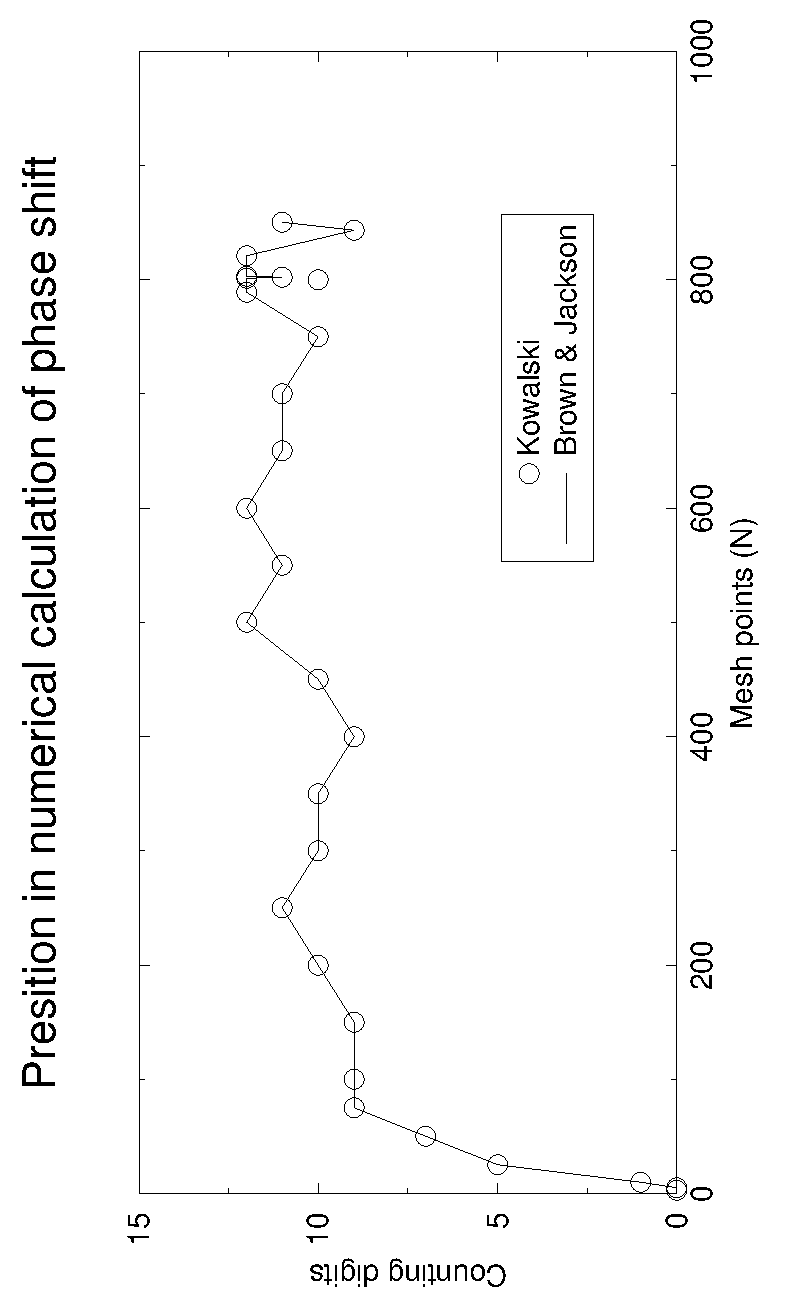
\includegraphics[height=15cm,angle=-90]{tellenesiffet.eps}
\caption{\label{figtellenesiffeta} Phase shifts in table~\ref{tabKowalskysammenlikning} 
are compared with a 12 digit phase shift which is
believed to be numerical correct.}
\end{figure}

%\newpage
%fig~\ref{fig:tellenesiffet}: Phase shifts in table ??? are compared with a 12 digit phase shift which is 
%believed to be numerical exact. 
\end{flushleft}



With mesh points less than 30, it seems like the difference between the phase shifts for the two methods
is less than 1.0E-13. It looks like the difference is slowly increasing with the number of mesh points. Which
is probably due to more numerical errors. Since the number of calculations done are increasing rapidly with N ($\sim N^3$). 
For 600 mesh points, when calculated for 15 different lab energies, the difference was found to be less than 1.0E-12. 
With N=843 the difference was in the order of 1.0E-7. 

Numerical errors can be divided into two parts. One due to the
to the accuracy in the integral calculation. This error will usually be less as N increase, and will depend on the potential.
The other part is due to the error all the numerical roundoff
errors will make, and this will be more or less independent of the potential. This error will, statistically, increase with N.
If we assume that the two methods generate independent errors, then the difference in the phase shifts will give us information
about the size of the numerical roundoff errors. 

The cases where the difference is 0, we clearly see that the assumption of independent roundoff errors
isn't always very good. For some mathematical-numerical reason "0" will turn up, even at large N.
To get the best estimate of the size of the error one should therefor study
each N with many energy-samples.
%But looking at other energies for the NN-interaction. In these cases, 
%we see that they are only statistical fenomenons*. 
%For some mathematical-numerical reason "0" will turn up, even at large N.
%At N=400 we have the first possible numerical roundoff error in order of 1.0E-8, but since the error is big
%compared with the phase shift difference, it is probably due to integral approximation errors.
In the table, the first obvious roundoff errors acoures in the Kowalski method for N=800. In this case
we have no mesh points close to $(q_{N+1})$. It is not the case it was created for. The normal method
gives very good result, and we clearly see the numerical round off errors acoures in the phase shifts. 
For N=843 both methods are involving
large round off errors. In this case there are two mesh points in the range of $(q_{N+1})\pm$1.0E-3. This is a situation
Kowalski had in mind when he recommended his method, and it is interesting to see that Kowalski was the best method in this case.

These errors doesn't
always acoures as big. It looks statistical like if something goes wrong, then a lot more will go wrong 
(Which is one of Murphys laws). 
But this doesn't happen to often (I believe Murphys laws never have proven to be correct, even though most of us experience different). 
For example $800\le N\le 850$ about 25$\%$ where such cases where the roundoff error blows up.
%Also the importance of a mesh point hitting close to the singularity seems to be small.

At N=789 there was one mesh point in the range of $(q_{N+1})\pm$1.0E-4. This was the only one one I could find in more than
a hundred tests. I was a little bit excited about how Kowalski would handle it. It did very well, but so did
the normal method. Both managed to reproduce the 12 first digits of the phase shift.
So the importance of a mesh point hitting close to the singularity seems to be small.

In summary the phase shifts in table~\ref{tabKowalskysammenlikning}  and fig~\ref{figtellenesiffeta} illustrates the facts:
\begin{itemize}
\item These methods are not only mathematically
equivalent, they are almost numerical identical to! With the Bonn Potential, one can trust about  
7 digits after the comma using mesh point between 200 and 600. But N=60 is good enough used on most potentials
on the marked today.
\item One should be careful using a large N (especially for N larger than 700), since this can reproduce
large numerical errors. If one need to find a higher precision of the phase shift,
one can look at an average of many samples with different N.
Or one can choose variables with better precision 
in the computer program, i.e. better than double precision.
\item Mesh points ending up as close as 5.0E-4 MeV to the singularity in the propagator seems to be of less importance
for the precision.
\item The methods use almost the same time.
\end{itemize}
 

These methods are almost numerical identical, and it is really hard to recommend one method over the other. 
Looks like Kowalski  was a little bit to worried about the numerical errors. The same can be said about Brown and Jackson.
In their book "Nucleon-Nucleon interaction" they also recommend the Kowalski method. Kowalski developed this
method in 1965. When Brown and Jackson recommended it in their book written in 1976,
computers that could handle more than a 100 mesh points didn't exist. And they would  not know if the problem was relevant
or not in real calculations.







%\end{flushleft} 

\kap{One Boson Exchange (OBE)}\label{chap:OBE}

The name of this model is misleading to the way it is being used today. Where it is 
a platform from where we can explane and simulate the strong force. The strong force is a product
of only meson exchanges. The weak force and EM force are created from other boson exchanges. So the name of the theory 
really says that it is a theory not only dealing with the strong force but also the weak force, EM force and even
gravitation (if the gravitation is a boson). This is however not the way this theory is build up, where all 
bosons except mesons are neglected. i.e. Leaving only the strong force.

The OBE model is an approximation of the real process where we have neglected higher order exchange diagrams.
It is normal to include the five lightest mesons in the model, and construct one fictive $\sigma$-meson.
The $\sigma$-meson then is supposed to include all the heavier mesons and also all the higher order meson exchange diagrams.
The potential vi can create from the OBE model is illustrated in  fig~\ref{figOBE}.
%\nl

\begin{figure}[!hbp]
\begin{center}
\begin{picture}(350,95)(0,0)
\Text(5,50)[l]{$\quad V_{{\text{OBE}}} =$}
\Text(55,50)[l]{$\quad\sum^{}_{\alpha=\pi,\eta,\rho,\omega,\delta,\sigma}\quad V^{{\text{OBE}}}_\alpha$}
\Text(190,50)[l]{$\equiv$} 
\Line(250,5)(250,95)
\Vertex(250,50){2}
\DashLine(250,50)(350,50){5}
\Line(350,5)(350,95)
\Vertex(350,50){2}
\Text(300,40)[c]{$\pi,\eta,\rho,\omega,\delta,\sigma$}
%\Text(160,50)[l]{$+$}
%\Line(180,5)(180,95)
%\Boxc(182,50)(4,40)
%\Text(190,50)[l]{$\Delta$}
%\DashLine(182,70)(240,70){5}
%\DashLine(182,30)(240,30){5}
%\Line(240,5)(240,95)
%\Text(210,80)[c]{$\pi,\rho$}
%\Text(210,20)[c]{$\pi,\rho$}
%\Text(250,50)[l]{$+$}
%\Line(270,5)(270,95)
%\Boxc(272,50)(4,40)
%\Text(280,50)[l]{$\Delta$}
%\DashLine(272,70)(330,70){5}
%\DashLine(272,30)(330,30){5}
%\Text(313,50)[l]{$\Delta$}
%\Line(330,5)(330,95)
%\Boxc(328,50)(4,40)
%\Text(300,80)[c]{$\pi,\rho$}
%\Text(300,20)[c]{$\pi,\rho$}
\end{picture}
\caption{\label{figOBE} \sl The standard OBE-model, where the five lightest mesons are included.
The $\sigma$-meson is artificial constructed to include an average of all the other possible exchanges.
Solid lines denotes nucleons.
}
\end{center}
\end{figure}

To calculate this potential, we need field theory, since particles with different spin will have different
properties. A correct model would involve QCD, since the mesons and nucleons are made up of quarks.
The fields we find from the mesons are therefor only an effective field, which only works for low energy NN interaction.
The mesons are grouped into different categories:
\begin{itemize}
\item Pseudo-scalar field ($ps$). Used for mesons with spin-0 like $\pi$ and $\eta$.
\item Scalar field ($s$). Mesons with spin-0 like $\delta$ and the fictive $\sigma$.  
\item Pseudo-vector field ($pv$). From a gradient coupling of the $ps$ field. 
This term is arising from
the chiral symmetry and is included as an effective $pv$ term.
In OBE models it is normal only to
include this effect in the $\rho$-meson and neglect the property in the $\omega$-meson. i.e. $f^\omega_{ps}=0$.
\item Vector field ($v$). Mesons with spin-1 like $\rho$ and $\omega$.
\end{itemize}
%The $\pi$ and $\eta$ are pseudo-scalar, $\sigma$ and $\delta$ are scalar, and $\rho$ and $\omega$ are vector
%mesons. For the $ps$ field, we also get a gradient coupling to the nucleon. This term is arising from
%the chiral symmetry and is included as an effective $pv$ term.

The Lagrangians that couples these fields can be found to be
\footnote{
Where
$\gamma^0=\left(
\begin{array}{rr}
1&0\\
0&-1
\end{array}\right)
$,
$\gamma^k=\left(
\begin{array}{rr}
0&\sigma^k\\
-\sigma^k &0
\end{array}\right)
$. The Pauli matrices($\sigma^k$) are:
%
$\sigma^1=\left(
\begin{array}{rr}
0&1\\
1&0
\end{array}\right)
$,
$\sigma^2=\left(
\begin{array}{rr}
0&-i\\
i&0
\end{array}\right)
$ and
$\sigma^3=\left(
\begin{array}{rr}
1&0\\
0&-1
\end{array}\right)
$,
$\gamma^5=\gamma_5=\gamma^1\gamma^2\gamma^3=\left(
\begin{array}{rr}
0&1\\
1&0
\end{array}\right)$
and
$\sigma^{\mu\nu}=\frac{i}{2}[\gamma^\mu,\gamma^\nu]$
}
:
\begin{eqnarray}\label{eq:Lagrang-ps}
{\mathcal L}_{ps}&=&-g_{ps}\bar{\psi}i\gamma_5\psi\phi^{(ps)}\\
%\end{equation}
%\begin{equation}\label{eq:Lagrang-s}
{\mathcal L}_{s}&=&g_{s}\bar{\psi}\psi\phi^{(s)}\\
%\end{equation}
%\begin{equation}
\label{eq:Lagrang-pv}
{\mathcal L}_{pv}&=&-\frac{f_{ps}}{m_{ps}}\bar{\psi}\gamma_5\gamma^\mu\psi\partial_\mu\phi^{(ps)}\\
%\end{equation}
%\begin{equation}
\label{eq:Lagrang-v}
{\mathcal L}_{v}&=&-g_{v}\bar{\psi}\gamma^\mu\psi\phi^{(v)}_\mu-\frac{f_v}{4M}\bar{\psi}\sigma^{\mu\nu}\psi(
\partial_\mu\phi^{(v)}_\nu-\partial_\nu\phi^{(v)}_{\mu})
\end{eqnarray}
M is the nucleon mass, $\psi$ denotes the Dirac spinor field of the nucleon and $\phi$ are the respective meson fields.
All the Lagrangian include a coupling constant $f$ and $g$. These coupling factors are relative large compared with other coupling 
constants in physics since we here are dealing with coupling constants arising from
the strong force.
The fist term on the right hand side of eq(\ref{eq:Lagrang-v}) is called vector coupling($v$), the second
for tensor coupling($t$).

From  these Lagrangian we are able to calculate the amplitude. The easiest way to do find this amplitude is
to use Feynman diagrams in a helisety basis.
\begin{figure}[!hbp]
\begin{center}
\begin{picture}(200,110)(0,0)
%\Text(5,50)[l]{$\quad V_{{\text{OBE}}} =$}
%\Text(55,50)[l]{$\quad\sum^{}_{\alpha=\pi,\eta,\rho,\omega,\delta,\sigma}\quad V^{{\text{OBE}}}_\alpha$}
%\Text(190,50)[l]{$\equiv$}
\ArrowLine(0,10)(50,50)
\ArrowLine(50,50)(0,90)
\Vertex(50,50){2}
\DashLine(50,50)(150,50){5}
\ArrowLine(200,10)(150,50)
\ArrowLine(150,50)(200,90)
\Vertex(150,50){2}
\Text(100,60)[c]{$m_\alpha$}
\Text(100,40)[c]{$q'-q$} 
\Text(40,50)[r]{${}_{\Gamma_1}$}
\Text(160,50)[l]{${}_{\Gamma_2}$}
\Text(0,0)[c]{$E,{{\bf q}}$}
\Text(0,100)[c]{$E',{{\bf q}}'$}
\Text(200,0)[c]{$E,-{{\bf q}}$}
\Text(200,100)[c]{$E',-{{\bf q}}'$}
\end{picture}
\caption{\label{figOBEFeynman} \sl 
Feynman diagram of a one meson exchange between two nucleons in the center of mass system.
}
\end{center}
\end{figure}
%
\begin{equation}\label{eq:amplitudefein} 
\braketm{{{\bf q}}'\lambda'_1\lambda'_2}{V}{{{\bf q}}\lambda_1\lambda_2}= 
\frac{
\bar{u}_{\lambda'_1}(-{{\bf q}}')\Gamma_1{u}_{\lambda'_1}(-{{\bf q}})
\bar{u}_{\lambda'_2}(-{{\bf q}}')\Gamma_2{u}_{\lambda'_2}(-{{\bf q}}) 
}{(q'-q)^2-m_{\alpha}^2}
\end{equation}
Using the relativistic eigen states also known as Dirac spinors 
\begin{equation}
{u}_{\lambda'_s}({{\bf q}})=\bigg(\frac{E+M}{2M}\bigg)\left(
\begin{array}{rr}
1\\
\frac{{{\bf \sigma}}\cdot{{\bf q}}}{E+M}
\end{array}\right)\chi_s
\end{equation}
So that
\begin{equation}
{u}_{\lambda}({{\bf q}})=\bigg(\frac{E+M}{2M}\bigg)\left(
\begin{array}{rr}
1\\
\frac{2\lambda q}{E+M}
\end{array}\right)\ket{\lambda}
\end{equation}
where $\lambda=\lambda_1 $or$ \lambda_2$, where $\lambda_1=\frac{1}{2}$ and $ \lambda_2=-\frac{1}{2}$. We also have $\bar{u}=u^\dagger\gamma^0$

The operator $\Gamma$ from the vertex in the Feynman diagrams will there for be (when using the Lagrangian above)
\begin{eqnarray}\label{eq:Gamma-ps}
\Gamma_{ps}&=&-\frac{g_{ps}}{\sqrt{4\pi}}\gamma_5\\
%\end{equation}
%\begin{equation}\label{eq:Lagrang-s}
\Gamma_{s}&=&-\frac{g_{s}}{\sqrt{4\pi}}\op{1}\\
%\end{equation}
%\begin{equation}
\label{eq:Gamma-pv}
\Gamma_{pv}&=&-\frac{if_{pv}}{\sqrt{4\pi}}\gamma^5\gamma^\mu\\
%\end{equation}
%\begin{equation}
\label{eq:Gamma-v}
\Gamma_{ps}&=&-\frac{g_{v}}{\sqrt{4\pi}}\gamma^\mu+\frac{if_{v}}{\sqrt{4\pi}2M}\sigma^{\mu\nu}(p'-p)
\end{eqnarray}
It is also normal to use
\begin{equation}
\frac{g_{ps}}{f_{ps}}=\frac{2M}{m_{ps}}
\end{equation}
whitch is on-mass-shell predictions where the $ps$ and the $pv$ coupling are identical.

Since the meson model doesn't include the break down at high energies where we have to deal with quarks instead of
mesons, it is necessary to introduce a form factor ${\cal F}[({{\bf q}}'-{{\bf q}})^2]$. The form factor has to be applied at each meson-nucleon vertex,
which is the same as multiplying ${\cal F}^2[({{\bf q}}'-{{\bf q}})^2]$ to the amplitude from eq(\ref{eq:amplitudefein}). This will
give us an amplitudes that converges.
\begin{equation}\label{eq:formfactor}
{\cal F}_\alpha[({{\bf q}}'-{{\bf q}})^2]=\bigg(\frac{\Lambda^2_\alpha-m^2_\alpha}{\Lambda^2_\alpha+
({{\bf q}}'-{{\bf q}})^2}\bigg)^{n_\alpha}
\end{equation}
Where $\Lambda$ is the cutoff parameter/mass. It is normal to use different $\Lambda$ for the mesons
in the OBE-model.

INKLUDER V(p)!!!!!!!!!!!!!!!!!!!!!!!!!!!!!!!!








A convenient way to  estimate the different parameters like the cutoffs($\Lambda$) and the $\sigma$-meson, 
is to partial wave compose the potential. In this frame one can fit very accurately the different partial waves 
with the experimental ones.

When the Bonn B parameters are fitted we find the parameters to be something like in table(\ref{tabBonnBparametere}),
which also include the rest of the Bonn B parameters like mass and spin.
\begin{table}[!hbp]
\begin{tabular}{|l|c|r|c|c|c|c|c|}
\hline 
    & $m_\alpha$ [MeV]& $g_\alpha^2\quad$ &$\frac{f_\alpha}{g_\alpha}$&$\Lambda$ [MeV]&$n_\alpha$&$J^P$&I\\
\hline
$\pi$ & 138.03&14.4000&0.00&1700&1&$0^-$&1\\
\hline
$\rho$& 769.00&0.9000&6.10&1850&2&$1^-$&1\\
\hline
$\eta$& 548.80&3.0000&0.00&1500&1&$0^-$&0\\
\hline
$\omega$& 782.60&24.5000&0.00&1850&2&$1^-$&0\\
\hline
$\delta$& 983.00&2.4880&0.00&2000&1&$0^+$&1\\
\hline
$\sigma$& 720.00&18.3773&0.00&2000&1&$0^+$&0\\
\hline
\end{tabular}
\caption{
\label{tabBonnBparametere}
\sl Bonn B parameters for the minimal relativity equation. Mass (${{\text m}}$), 
width ($\Lambda$), coupling constants (f and g), spin (${{\text J}}$), parity (${{\text P}}$), isospin (${{\text I}}$) 
}
\end{table}

\kap{Experimental data}\label{chap:Experimental data}


The process in receiving the experimental data for the binding energy of nuclears
is straight forward and very accurate.
The experimental value of the binding energy of the Deuteron(${}^2$H) is $2.224589\pm0.000002$  MeV
This binding energy is found by measuring the energy of the $\gamma$-ray photon that is emitted when a free np-system is 
being bound.
\begin{equation}
p+n\rightarrow {}^2{\text{H}}+\gamma
\end{equation}
One can also find an binding estimate for the opposite process where a $\gamma$-ray photon breaks apart the deuteron
This method is called photodissociation. A third way to measure the binding energy is by doing spectroscopy and using the
mass doublet method described in \cite{roed}. 
These three methods are all in excellent agreement, but the last two methods are not as accurate as the first one.
\nl
Evaluating phase shifts, mixing parameters and inelasticities are on the other hand a much more complicated process.
The observable in a NN-scattering like the partial cross sections and polarizations give us enough
parameter to describe the scattering experimentally. But in order to find the phase shifts, the mixing parameters  and
inelasticities, one have to 
do a partial wave decomposition. This method is far from being accurate, and the errors are getting bigger with
the energy in the scattering. The accuracy is getting better and better as new experimental and better data
are used. So every now and then a new updated version is made. The
same people are usually publishing these updates, since they all-ready a computer program. Therefor they only 
have to update the observable with new and better ones.

It is also possible to go the other way from phase shifts and inelasticities to cross section. For example
obs.f written by ??? calculates the scattering observable from the phase shifts.

This process is difficult, and is perhaps illustrated in R.A.Arnts
phase shifts analysis from 2000 ~\cite{PRC62faseskift3GeV}.
Where the \state{3}{D}{1} state differences in the inelasticity between experiments and theory 
can be due to a sign convention (REF FIGUR!!!!).
Machleidt who wrote the theoretical "nna13" potential, strongly believes that Arndt have done a mistake in his 
sign convention for this state.
\nl
How the accuracy in phase shift variates, can be seen from phase shift analysis from 1993 
~\cite{PRC48faseskift350MeV}.
%\nl
%\begin{flushleft}
\begin{table}
\begin{tabular}{|l|c|c|c|c|}
\hline
 & \multicolumn{2}{|c|}{ pp phase shifts} &\multicolumn{2}{|c|}{ np phase shifts}\\
 \hline
$T_{lab}$& \state{1}{S}{0} & \state{3}{F}{2}& \state{1}{S}{0} & \state{3}{S}{1}\\
\hline
1 MeV& $32.684\pm0.005$& 0.000&$62.068\pm0.030$& $147.747\pm0.010$\\
\hline
100 MeV&$24.97\pm0.08$& $0.817\pm0.004$&$26.78\pm0.38$&$43.23\pm0.14$\\
\hline
200 MeV&$6.55\pm0.16$& $1.424\pm0.034$&$8.94\pm0.39$&$21.22\pm0.15$\\ 
\hline
350 MeV& $-11.13\pm 0.46$& $1.04\pm 0.16$&$-10.59\pm 0.62$&$0.502\pm0.32$\\
\hline
\end{tabular}
\caption{
\label{tableexperiment} 
Experimental proton-proton and neutron-neutron phase shifts.
Uses phase shift data from ~\cite{PRC48faseskift350MeV}.}
\end{table}
%\end{flushleft}


We see from table~\ref{tableexperiment} that the phase shift accuracy is better for pp than np scattering.
This is due to the fact that it is much easier to handle protons than neutrons. 
For example both giving the nucleons a known initial energy, and observing the
nucleons after the scattering are much more complicated for neutrons than protons.
nn-scattering data does not exist because of these difficulties with the neutron.
For the \state{1}{S}{0} states the error estimate of the phase shift is less than 10$\%$
when compared with the phase shift. 
The errors are about four times as big in the nn-scattering as it is for pp-scattering. 
The \state{3}{F}{2} state and \state{3}{S}{1} illustrates smaller phase shifts where
the the error estimate is about 50$\%$ of the phase shift. In 
\ref{fig:hiEnergy} we have the same problem with the inelasticity in the
\state{3}{D}{2} state. In this state the inelasticities are so small compared with their corresponding
uncertainty, so Arndt have set them to zero in his article ~\cite{PRC62faseskift3GeV}.


Experimental phase shifts for higher energies up to 3 GeV are given in ~\cite{PRC62faseskift3GeV}.
\nl
Phase shifts in-medium are still not calculated experimentally. 
\nl
Polarization scattering experiments are done by a polarizing the particles spin, so that one can study the
spin dependence in the scattering.
 
 
\kap{NN-scattering up to 1 GeV}\label{chap:NN-scattering up to 1 GeV}


There can be some inelasticity from Bremsstrahlung ($N+N\to N+N+\gamma)$ in the scattering.
This term is small and will diaper when we neglect the electromagnetic force. Larger inelasticity
are entering the picture for lab energies about 300 MeV.
This is due to
fact that at 300 MeV, nucleons have enough energy to create a free $\pi$-meson ($N+N\to N+N+\pi$).
At higher
energies creations of other mesons will also enter the process.
Creation of such mesons will also have an effect on the phase shifts.

At 600 MeV creation of two $\pi$-mesons are possible, but at this energy another important factor to the inelasticity
can arrive.
This is due to the the excitations of one the nucleons into $\triangle$(1232).
%If the state is virtually excited to $\triangle$, the virtual state can fall back to the ground state (N). In this process, 
%there will be created a free meson in the process.
%This has such a big effect on the inelasticity since it doesn't only slow down the speed of the nucleons, which is what the
%$\pi$-mesons does. $\triangle$ excitation also remove one nucleon in the process.
%But the biggest contribution to the
%inelasticity at higher energies is the 2 mesons exchange that can change one of the incoming nucleons. At
%lab energies around 600 MeV we can get the 2 $\pi$ exchange through the process
$N+N\to N+\triangle$. 
Because of isospin addition rules, this process is only possible with a two nucleon state with isospin $I=1$.
%Where $\triangle$ has the same barion number and the total isospin as the nucleon N it replaced.

If the state is virtually excited to $\triangle$, the virtual state can fall back to the ground state (N). In this process,
there will be created a free meson in the process.

There exist four $\triangle$-barions
and they come from the isospin-$\frac{2}{3}$ barion group.
They can be expressed in terms of quarks as $\triangle^-={\textrm{ddd}}(I_3=-3/2)$,\;$\triangle^-=\textrm{udd}(I_3=-1/2)$,
\;$\triangle^-={\textrm{uud}}(I_3=1/2)$ and $\triangle^{++}={\textrm{uuu}}(I_3=3/2)$. Where $I_3$ is related to the particles
electrical charge. This quatety is concerved since the charge is conseved.
%If we assume that the isospin is a good quantum number. i.e. we neglect the decays done by the
%electromagnetic and the week force.
For the barion dublet we have $n$($I_3=-1/2$) and $p$($I_3=1/2$).
%
%We therefor have that $p+p\to p+\triangle^{+}$ is one of the possible $\triangle$ excitations.
%
At energies above 1,2 GeV we can get double $\triangle$ excitations ($N+N\to \triangle+\triangle$).
This process is posible for states with both isospin 0 and 1.
If we want to include the inelasticety caused by a one or a two 
$\triangle$ exitation using a real potential like the "bonn B"-potential
, we have to include the width $im^{{\text imag}}_\triangle$ 
of the $\triangle$-barions in the propagators of the coupled $\LS$ equation.
This width (self-energy) will be a complex componet
of the energy/mass. 
\begin{equation}
m_\triangle=m^{{\text real}}_\triangle+im^{{\text imag}}_\triangle
\end{equation}
The real part will be the same as before. 







\section{Coupled Channels And The "nna13"-Potential}
If we want to include the viretual $\triangle$-excitations, we need
to include two mesons exchange deagrams to the OBEP moddel. This is shown in
fig~\ref{figVnna13}, where only the creation of $\pi$ and $\rho$ are included.
BEDREEEEEEEEThe self-energy model is
equivalent to three body Feynman diagrams were mesons are emitted in the process.
This will give a coupled
channel vertion of the $\LS$ equation, which is
\begin{eqnarray}
{T}_{NN,NN}=V_{NN,NN}&-&\int d^3k\frac{V_{NN,NN}{T}_{NN,NN}}{\varepsilon_{NN}-\varepsilon^0_{NN}}
-\int d^3k\frac{V_{NN,N\triangle}{T}_{N\triangle,NN}}{\varepsilon_{N\triangle}-\varepsilon^0_{NN}}\nonumber\\
&-&\int d^3k\frac{V_{NN,\triangle\triangle}{T}_{\triangle\triangle,NN}}{\varepsilon_{\triangle\triangle}-\varepsilon^0_{NN}} 
\end{eqnarray}
where  
\begin{eqnarray}
{T}_{N\triangle,NN}=V_{N\triangle,NN}&-&\int d^3k\frac{V_{N\triangle,NN}{T}_{NN,NN}}{\varepsilon_{NN}-\varepsilon^0_{NN}}
-\int d^3k\frac{V_{N\triangle,NN}{T}_{N\triangle,NN}}{\varepsilon_{N\triangle}-\varepsilon^0_{NN}}\nonumber\\
&-&\int d^3k\frac{V_{N\triangle,\triangle\triangle}{T}_{\triangle\triangle,NN}}{\varepsilon_{\triangle\triangle}-\varepsilon^0_{NN}}
\end{eqnarray}
and all the other ${T}_{xx,xx}$ are calculated similary. To calculate these equations we need to have an expression for
all the different potentials $V_{xx.xx}$ like $V_{NN,N\triangle}$ and $V_{NN,\triangle\triangle},\cdots$. 
\begin{equation}
\varepsilon_{N\triangle}=E_{{\text N}}+E_\triangle
\end{equation}
where
\begin{equation}
{{\text E}}_{{\triangle}} =\frac{k^2}{2m_{{\triangle}}}+m_{{\triangle}}
\end{equation}
,
\begin{equation}
{{\text E}}_{{\text N}} =\frac{k^2}{2m_{{\text N}}}+m_{{\text N}}
\end{equation}
and the on-shell energy is
\begin{equation}
\varepsilon^0_{NN}=2\bigg(\frac{q^2_0}{2m_{{\text N}}}+m_{{\text N}}\bigg)
\end{equation}

To calculate all the coupled channels is a pretty lenthy task. Since the one $\triangle$-excitation
is much more important for the inelastic system below 1 GeV, one can make the coupled channel problem easier by
neglecting the double $\triangle$-excitations, or
%instead of doing all this, 
one can also make use of the complex
potentials all ready on the marked. Machleidts "nna13"-potential for 
example. This potential is relatively good up to 1 GeV, and
includes both one and two virtual $\triangle$ excitations. 
%This self-energy model is
%equivalent to three body Feynman diagrams were mesons are emitted in the process. 
%The propagator between a 
%excited $\triangle$ and a N is implemented in nna13, and is on the form
The nna13 potential has been written so that one can use the uncoupled $\LS$ equation
with the same propagator as in the OBE potential
\begin{equation}
{{\text G(E)}}=\frac{1}{\varepsilon_{NN}-\varepsilon^0_{NN}}
%\frac{1}{z_0-E_\triangle-E_{{\text N}}}
\end{equation}
%where 
%\begin{equation}
%{{\text E}}_{{\triangle}} =\frac{k^2}{2m_{{\triangle}}}+m_{{\triangle}} 
%\end{equation}
%,
%\begin{equation}
%{{\text E}}_{{\text N}} =\frac{k^2}{2m_{{\text N}}}+m_{{\text N}} 
%\end{equation}
%and the on-shell energy is
%\begin{equation}
%z_0=2\bigg(\frac{q^2_0}{2m_{{\text N}}}+m_{{\text N}}\bigg)  
%\end{equation}
%The propagator in the  $\LS$ equation will be the same as before, since we still the same NN-propagator.
%One can therefor explane the small
%inelasticity at low enegies, by the small self-energies of N.
At higer energies also effects like N* (Roper resonance) has to be included.

The one boson exchange diagrams of the nna13 potential is build up as shown in fig~\ref{figVnna13},
where also the two exchange diagrams of the $\triangle$ excitation are included.
The nna13 potential also include the cdbonn package (\ref{cdbonn}), which means that the nna13 potential is also 
including the charge dependece in the scattering. This way
the nna13 potential is fitted better to the experimental data than a plane OBE potential. 

This is based on a field theoretic model, where only the lowest $\triangle$/(N$\pi$) excitations are taken into account.
The fictive $\sigma$-meson is taken apart, so we can seperate the processes that causes creation of the lightest mesons.
Of these new $\triangle$ diagrams, the 2$\pi$ exchanges are 
the most important effect.
Also the $\pi\rho$ and $\rho\rho$ exchange diagrams are important. 
From OBEP the diagrams of one and two $\triangle$ excitation
are removed from the $\sigma$. The new $\sigma'$ is therefor a little different from the $\sigma$ from the OBE.
These changes are included in the nna13 potential to describe the effect of the inelastic part of the scattering.
\nl
\begin{figure}{}
%\begin{center} 
\begin{picture}(330,95)(0,0)
\Text(5,50)[l]{$V_{NN} =$}
\Line(50,5)(50,95)
\Vertex(50,50){2}
\DashLine(50,50)(150,50){5}
\Line(150,5)(150,95)
\Vertex(150,50){2} 
\Text(100,40)[c]{$\pi,\eta,\rho,\omega,\delta,\sigma '$} 
\Text(160,50)[l]{$+$}
\Line(180,5)(180,95)
\Boxc(182,50)(4,40)
\Text(190,50)[l]{$\Delta$}
\DashLine(182,70)(240,70){5}
\DashLine(182,30)(240,30){5}
\Line(240,5)(240,95)
\Text(210,80)[c]{$\pi,\rho$}
\Text(210,20)[c]{$\pi,\rho$}
\Text(250,50)[l]{$+$} 
\Line(270,5)(270,95)
\Boxc(272,50)(4,40)
\Text(280,50)[l]{$\Delta$}
\DashLine(272,70)(330,70){5}
\DashLine(272,30)(330,30){5}
\Text(313,50)[l]{$\Delta$}
\Line(330,5)(330,95)
\Boxc(328,50)(4,40) 
\Text(300,80)[c]{$\pi,\rho$}
\Text(300,20)[c]{$\pi,\rho$}
\end{picture} 
\caption{\label{figVnna13} \sl The three body diagram of the OBE part of the nna13 potential and the two meson exchange
$\triangle$-excitation diagrams. All of higer order diagrams have been neglected.
Solid lines denotes nucleons.
The first diagram on the left hand side is a one meson exchange diagram, and the two others are excited states
of the two meson exchange diagrams.} 
%\end{center}
\end{figure}

The fig~\ref{figVnna13}
is a three body equation. As mentioned before nna13 uses a coupled two-body channel model which is almost equivalent to
the three body equations.
LAG NY FIGUR!!!!!!!!!!!!!!!!!!!!
\nl
The results of the first phase shifts and inelasticities with the nna13 potential are plotted in \ref{fig:hiEnergy}. 
From these data one can calculate the cross section. The total cross section($\sigma$) will be dependent on all the partial waves. 
However the cross section calculated from the phase shifts converges. The importance of
the phase shifts and inelasticity as J increases are shown in tab~\ref{tabcrossel} and tab~\ref{tabcrossinel},
where the program "obs.f" has been used.

\begin{table}[!hbp]
\begin{tabular}{|l|c|c|c|c|c|}
\hline
& \multicolumn{5}{|c|}{$\sigma_{NN-elastic}$ $[mb]$}\\
\hline
$T_{lab}$& { $J_{max}=3$}  & { $J_{max}=10$} & { $J_{max}=20$} & $J_{max}=80$ & Experimental\\
\hline
200 MeV&40.254595&41.849377 &41.851221  &41.851221 &42.78\\
\hline
%300 MeV &35.036848 & & & &32.40\\
%\hline
400 MeV&29.286240&32.212076 &32.228529  &32.228552 &32.40\\
\hline
%500 MeV &30.310964 & & & &26.25\\ 
%\hline
600 MeV&24.781240&28.080876 &28.120242  &28.120412 &29.54\\
%\hline
%700 MeV &26.083066 & & & &\\
\hline
800 MeV&21.486933&24.551982 &24.614851  &24.615376 &26.25\\
%\hline
%900 MeV &23.598118 & & & &\\
\hline
1000 MeV&20.521614&23.093538 &23.177359 & 23.178458 &23.29\\ 
\hline
\end{tabular}
\caption{
\label{tabcrossel}
\sl Total elastic cross section from np scattering using the nna13 potential and all the partial waves up to $J_{max}$. 
Experimental values \cite{PRC62faseskift3GeV}  are also included}
\end{table}
%
%
\begin{table}[!hbp]
\begin{tabular}{|l|c|c|c|c|c|}
\hline
& \multicolumn{5}{|c|}{$\sigma_{NN-elastic}$ $[mb]$}\\
\hline
$T_{lab}$& $J_{max}=3$  & $J_{max}=10$  & $J_{max}=20$ & $J_{max}=80$ & Experimental\\
\hline
200 MeV&0.000000&0.000000 &0.000000  &0.000000 &0.0000\\
%\hline
%300 MeV &0.006844 & & & &\\
\hline
400 MeV&0.477711&0.518062 &0.518062  &0.518062 &0.6947\\
%\hline
%500 MeV &2.429705 & & & &\\
\hline
600 MeV&6.036612&6.706089 &6.707221  &6.707221 &6.479\\
%\hline
%700 MeV &9.410750 & & & &\\
\hline
800 MeV&8.879003&11.032602 &11.040103  &11.040103 &12.37\\
\hline
%900 MeV &12.442983 & & & &\\
%\hline
1000 MeV&9.815736&13.053151&13.074315  &13.074315 &15.45\\
\hline
\end{tabular}
\caption{
\label{tabcrossinel}
Total inelastic cross section from np scattering using the nna13 potential and all the partial waves up to $J_{max}$.
Experimental values \cite{PRC62faseskift3GeV}  are also included}
\end{table}


%\begin{equation}\label{eq:probforelastic}
%N+N\to N+N
%\end{equation}
%This is the elastic process. All the other processes are inelastic. $|\eta_l|^2$ can therefor be interpreted as the
%probability of elastic scattering (\ref{eq:probforelastic}). This definition of
%inelasticity does not contain any information about the relation of all the other inelastic processes. Like
%the probability of one pion or two pion creation in the scattering.


For higher energy scattering, we also have to include the substructure of the Hadrons. This model has to be based on quarks, 
and the OBE model is no longer sufficient to describe the NN-scattering process. 



\begin{flushleft} 
\begin{figure}%\label{fig:hiEnergy}
%\centering
\begin{flushleft} 
\includegraphics[height=20cm,width=18cm]{figd85_alt1.ps} 
\end{flushleft}  
%\caption{\state{1}{S}{0} phase shifts for a box Potential, a parameterized potential, the Bonn B potential and
%experimental data ~\cite{PRC48faseskift350MeV}. How the potentials are build up
%will be explained later.}
\end{figure}
\end{flushleft}

\begin{flushleft}
\begin{figure}%\label{fig:hiEnergy}
%\centering
\begin{flushleft}
\includegraphics[height=20cm,width=18cm]{figd85_alt2.ps}
\end{flushleft}
%\caption{\state{1}{S}{0} phase shifts for a box Potential, a parameterized potential, the Bonn B potential and
%experimental data ~\cite{PRC48faseskift350MeV}. How the potentials are build up
%will be explained later.}
\end{figure}
\end{flushleft}

\begin{figure}%\label{fig:hiEnergy}  
%\centering
\begin{flushleft}
\includegraphics[height=20cm,width=18cm]{figd85_alt3.ps}
\end{flushleft}
%\caption{\state{1}{S}{0} phase shifts for a box Potential, a parameterized potential, the Bonn B potential and
%experimental data ~\cite{PRC48faseskift350MeV}. How the potentials are build up
%will be explained later.}
\end{figure}

\begin{figure}%\label{fig:hiEnergy}
%\centering
%\begin{flushleft}
\includegraphics[height=20cm,width=18cm]{figd85_alt4.ps}
%\end{flushleft}
\caption{\label{fig:hiEnergy} Theoretical phase shifts and inelasticities for a OBE potential ("cd-bonn")
that includes N-$\triangle$ and $\triangle$-$\triangle$ box diagrams. This complex potential is called "nna13"
and was written by R. Machleidt in 2000. The dots are experimental values. Where the black dots are taken 
from \cite{PRC48faseskift350MeV}, and
the white dots from \cite{PRC62faseskift3GeV}}
\end{figure}

\kap{In-Medium Scattering}\label{chap:In-Medium Scattering} 
So far only free NN scattering has been considered. From this data there have built different potential
like the nna13 potential, which is fairly good up to 1 GeV. Since the strong force is a three body force, we will
experience different potential between two free nucleons than two nucleons in a nuclear with three or more nucleons. 
However, most of the many-body theory today is based on the potential made from simple NN-systems.

The spherical geometry and the boundary conditions 
of the nuclears, makes it difficult to make a mathematical model of the situation. A commonly used 
simplification to the problem, is to introduce
the theoretical "nuclear matter"-model. This model is very similar to the situation inside heavy nuclears.
In order to describe the situation one also have to include properties from many particle theory 
like the Pauli effect and the dispersion effect.
\section{Nuclear Matter}
Nuclear matter is from definition  a infinite system nucleons, which are only interacting through the strong force,
i.e. all the other forces are neglected. This situation is an approximation to the real situation we
have in heavy nuclears. Nucleons in the boundary of the nuclear will behave slightly different, 
and the approximation will be better the closer the nucleon are to the center of the heavy nuclear.
A nice mathematical property of the nuclear matter model is that such a system is translation invariant.

The non relativistic Hamiltonian of an interacting many-particle system is
\begin{eqnarray}\label{eq:first-quant}
\op{H}&=&\op{T}+\op{W}+\op{V}\nonumber\\
      &=&\sum^N_{i=1}\frac{{{{\bf p}}}^2_i}{2m}+\sum^N_{i=1}w({{\bf r}}_i)+\sum^N_{i<j}v({{\bf r}}_i,{{\bf r}}_j)
\end{eqnarray}
Where $N$ is the number of particles in the system. For a translational system we must have
\begin{equation}
w({{\bf r}})={\text{constant}}
\end{equation}
This is precisely what we achieve in creating a uniform system like the nuclear matter model. Where the
potential from the nucleons position in the nuclear matter is the same for all the nucleons because there are no boundary effects 
in this model, and the nuclear matter is symmetric. If we also assume that there are non external potential to the system,
we have $w({{\bf r}})=0$

In the nuclear matter model the single particle waves can be expressed in plane waves instead of self-consistent Hartree-Fock wave
functions we get from solving the exact problem with heavy nuclears.
The eigenfunction of plane waves are
\begin{equation}
\phi_{{\bf {k}}\sigma}(x)=\frac{1}{\sqrt{\Omega}}e^{i{\bf {kr}}}\chi_\sigma(s)
\end{equation}
Where $\sigma(s)$ denotes the usual Pauli-spinor and $\Omega$ is the volume element we need to normalize the wave function.
In second quantization \ref{eq:first-quant} can be rewritten
as
\begin{eqnarray}\label{eq:seceond-quant}
\op{H}&=&\sum_{{{\bf {k}}\sigma}}\bigg(\frac{{\bf {k}}^2}{2m}+w\bigg)
\op{c}^\dagger_{{{\bf {k}}\sigma}}\op{c}_{{{\bf {k}}\sigma}}
\nonumber\\
      &&+\frac{1}{2\Omega}\sum_{{\bf {q}}}\sum_{{{\bf {k}}\sigma},{{\bf {k}}'\sigma'}}
      v_{{\bf {q}}}
      \op{c}^\dagger_{({{\bf {k}}+{{\bf {q}}})\sigma}}\op{c}^\dagger_{({{\bf {k}}'-{{\bf {q}}})\sigma'}}
      \op{c}_{{{\bf {k}}'\sigma'}} \op{c}_{{{\bf {k}}\sigma}} 
\end{eqnarray}

To get the nuclear matter model as close to the real situation in the interior of a heavy nuclear, the nuclear matter density
is chosen to be the same as the observed one in heavy nuclears.
\begin{equation}
\rho=0.17\pm 0.02\quad {\text fm}^{-3}
\end{equation}
The Fermi momentum $k_F$ can be defined as
\begin{equation}
k^3_F=\frac{3}{2}\rho\pi^2
\end{equation}
From these two equations we have
\begin{equation}
k_F=1.35\pm0.05\quad {\text fm}^{-1}
\end{equation}
The Fermi momentum is an important factor in the phase shift analysis, which arrives from the Pauli effect in medium.









\section{Many-body Theory}
The theory dealt with here is constructed from the wish of explaining the the interactions through a
two-body potential. So that we can use the potential from the NN interaction to explain all the different nucleon configurations, 
or that is at least the ultimate goal of the theory.

The perturbation theory is developed around the Hartree-Fock approximation, where the unperturbated Hamiltonian $H_{\text{HF}}$
is the effective single particle Hamiltonian. Eq(\ref{eq:first-quant}) can then be written as
\begin{eqnarray}\label{eq:HF-approx}
\op{H}&=&\sum^N_{i=1}\bigg( \op{t}_i+\op{u}_i\bigg)+\bigg(\sum^N_{i<j}\op{v}_{ij}-\sum^N_{i=1}\op{u}_i\bigg) \nonumber\\   
      &=&\op{H}_{\text{HF}}+\op{H}'
\end{eqnarray}
Where the external potential is neglected. $\op{H}'$ is the perturbation.
Since the nucleons are Fermions, one have to use Slater determinants of single-particle orbitals as a basis for
the total many body wave function. These Slater determinants should also include the Pauli spinor, so that 
spin properties of the system is accounted for.
This way the Hamiltonian ${\op{H}}$ will commute with the square and the z-component 
of the total angular momentum and total spin. 
One can calculate the expectation value of $\op{H}$ with a Slater determinant basis (${{ \Phi}}$). Here written in second quantization
\begin{equation}\label{eq:HF-sec} 
\braketm{{{ \Phi}}}{\op{H}}{{{ \Phi}}}
=\sum^N_{i=1}\braketm{i}{h_{HF}}{i}+\frac{1}{2}\bigg(\sum^N_{i,j=1}\braketm{ij}{v}{ij}-\sum^N_{i,j=1}\braketm{ij}{v}{ji}\bigg) 
\end{equation}
We see that the interaction potential consists of two terms. It has been normal to call
the first term in the brackets in (\ref{eq:HF-sec}) for the direct term. The second is called the exchange term.
UFERDIG!!!!!!!!!!!!!!!





\section{Minimal Relativity With Build-In Dispersion Effect}
The Minimal relativity equation in free space is
\begin{equation}\label{eq:Trelllllfree}
\braketm{{ p}} {\op{T}_l(E_{ k})}{{ k}}=\braketm{{ p}}{\op{V}_l}{{ k}}
+ \frac{2}{\pi}%\;{\cal P}
\int^{\infty}_{0}d { q}\; q^2\bra{{ p}}\op{V}_l\ket{{ q}}
\;\inv{{\varepsilon(k)}-{\varepsilon(q)\pm i\epsilon}}   \;\bra{{ q}} \op{T}_l(E_{ k})\ket{{ k}}
%\nonumber\\
%&&
%-i { k}m \bra{{ p}}\op{V_l}\ket{{ k}}
%\;\bra{{ k}}\op{T}_l(E_{ k})\;\ket{{ k}}
\end{equation}
where $\varepsilon(k)$ is the free two nucleons energy in the center of mass 
\begin{eqnarray}
\varepsilon(k)=\frac{k^2}{m_{{\text N}}}+m_{{\text N}}
\end{eqnarray}
In a medium this energy can be written as a dispersion relation, where the energy is a function of the momentum
\begin{eqnarray}\label{eq:inmediumeps}
\widetilde{\varepsilon}(k)=\frac{k^2}{m_{{\text N}}}+m_{{\text N}}+U(k)
\end{eqnarray}
The potential $U(k)$ arises because the nucleons interact with the nuclear matter. This potential will be negative
for small k (i.e feels an attractive force from the nucleons in the nuclear matter. The potential
is found to be on the form  
\begin{eqnarray}
U(k)\approx {{\text c}}k^2-U_0
\end{eqnarray}
Where c is a constant.
With this approximation we can rewrite  (\ref{eq:inmediumeps}).
\begin{eqnarray}\label{eq:inmediumeps2}
\widetilde{\varepsilon}(k)=\frac{k^2}{m^*_{{\text N}}}+m_{{\text N}}-U_0
\end{eqnarray}
The effective mass $m^*$ is a commonly used in many particle models. In nuclear matter it is found
to be about 688 MeV. This is done by using Brecner theory, where one first guess a $m^*_{{\text N}}$ to use. 
From the theory one can then calculate a better $m^*_{{\text N}}$, which one use again and again until self consistent is achieved.
More about this both relativistic and non relativistic are explained in~\cite{Macbok}.
The propagator term in the $\LS$ equation will be dependent on the difference of $\widetilde{\varepsilon}(k)$ 
and $\widetilde{\varepsilon}(q)$. This effect is called "Dispersion effect" 
\begin{eqnarray}\label{eq:inmediumeps3}
\widetilde{\varepsilon}(k)-\widetilde{\varepsilon}(q)=\frac{k^2}{m^*_{{\text N}}}-\frac{q^2}{m^*_{{\text N}}}
\end{eqnarray}
The new $\LS$ equation with this Dispersion effect included, will be
\begin{eqnarray}\label{eq:Trelllllnoererw}
\braketm{{ p}} {\op{T}_l(E_{ k})}{{ k}}&=&\braketm{{ p}}{\op{V}_l}{{ k}}
+ \frac{2m^*_{{\text N}}}{\pi}\;{\cal P}\int^{\infty}_{0}d { q}\; q^2 \quad\bra{{ p}}\op{V}_l\ket{{ q}}
\;\inv{{ k^2}-{ q^2}}   \;\bra{{ q}} \op{T}_l(E_{ k})\;\ket{{ k}}\nonumber\\
&&
-i { k}m^*_{{\text N}} \bra{{ p}}\op{V_l}\ket{{ k}}
\;\bra{{ k}}\op{T}_l(E_{ k})\;\ket{{ k}}
\end{eqnarray}
For the relation between the on-shell momentum k in the center of mass system and the lab energy $T_{{\text lab}}$
is the same as before. Namely,
\begin{eqnarray}
k=\sqrt{\frac{m_{{\text N}}T_{{\text lab}}}{2}}
\end{eqnarray}
Where m is again the free mass of a nucleon.




\section{The Pauli Effect in nuclear matter}
The Pauli effect is a direct consequence of the Pauli principal and the model we use to describe the nuclear matter.
If we assume that all the nucleons in the nuclear matter are in the lowest eigen states possible, and we name
the state whit the highest energy to be the Fermi momentum $k_{{\text F}}$. Because of the
Pauli principal, all the interacting nucleons have to be in different energy states. If the energy states up till
$k_{{\text F}}$ are occupied by the nucleons in the nuclear matter, the allowed energy states for
the nucleons being scattered have all $k\ge k_{{\text F}}$. In operator form we include the Pauli operator $Q$
in the propagator in the $\LS$ equation from   (\ref{eq:TM}) 
\begin{equation}\label{eq:TM22222}
\op{T}=\op{V}+\op{V}Q\op{G}^{}_0\op{T}
\end{equation}
The Pauli operator $Q$ projects only onto the unoccupied states. In partial wave decomposition in
momentum space this will be
\begin{equation}\label{eq:Trelllllinmed}
\braketm{{ p}} {\op{T}_l(E_{ k})}{{ k}}=\braketm{{ p}}{\op{V}_l}{{ k}}
+ \frac{2m^*_{{\text N}}}{\pi}%\;{\cal P}
\int^{\infty}_{k_{{\text F}}}d { q}\; q^2\bra{{ p}}\op{V}_l\ket{{ q}}
\;\inv{{k^2}-q^2\pm i\epsilon}   \;\bra{{ q}} \op{T}_l(E_{ k})\ket{{ k}}
%\nonumber\\
%&&
%-i { k}m \bra{{ p}}\op{V_l}\ket{{ k}}
%\;\bra{{ k}}\op{T}_l(E_{ k})\;\ket{{ k}}
\end{equation}
Where also the dispersion effect has been included.





\section{Dispersion Effect involving $\triangle$-excitations} 
The next step will be to include the effective mass of the nucleons in the
$\triangle$-excitations diagrams. By including the in-medium effect in the one $\triangle$-excitation
propagator $\widetilde{\epsilon}_\triangle$ in the coubled channel equation. 
\begin{equation}\label{eq:TM22222344444444}
\frac{1}{\widetilde{\epsilon}_{{\text N}}({{ k}})+
\widetilde{\epsilon}_\triangle({{ k}})-2\widetilde{\epsilon}_{{\text N}}({{ k}}_0)}
\end{equation}
Where $\widetilde{\epsilon}_{{\text N}}({{ k}}_0)$ is the total energy in the center of mass system.
The two $\triangle$-excitation if included should also be changed in the same way.
If we neglect the in-medium effect on the $\triangle$ particles, which was also done for the mesons
\begin{equation}
\widetilde{\epsilon}_\triangle={\epsilon}_\triangle=\frac{{{ k}}^2}{2m_\triangle}+(m_\triangle-m_{{\text N}})  
\end{equation} 
Where ${\cal R}{e}[m_\triangle]=1232$ MeV. The in medium effect on the propagator in (\ref{eq:TM22222344444444})
is therefor only in the $\widetilde{\epsilon}_{{\text N}}({{ k}})$ part, which is given in
(\ref{eq:inmediumeps2}).

This in-medium effect has been built in to the potential nna13 and this version is called nna13in. 





\section{Numerical Solution Of In Matter Scattering}

The Dispersion effect is included in the computer program if all the Nucleon masses ($m=m_{{\text N}}$) 
are changed to the effective mass ($m^*=m^*_{{\text N}}$), except in the calculation of the on-shell momentum in
the center of system $k({{\text N}}+1)$.

The Pauli effect is included by changing the integral from $(0,\infty) \to (k_{{\text F}},\infty)$.
Numerically this can be done by adding $k_{{\text F}}$ to all the mesh points (not to $k({{\text N}}+1)$),i.e.
\begin{equation}\label{eq:TM2222233333}
q_i=q_i+k_{{\text F}},\qquad {{\text for}}\quad i\le N
\end{equation}
Where N is the number of mesh points.
By changing the integral limits, we also change the limits on the term that numerically removes the singularity
in the integrand (\ref{eq:trix0}). 
\begin{equation}\label{eq:trix022222}
-\frac{2m^*}{\pi}\;k^2\bra{{ p}}\op{V}_l\ket{{ k}}
\bra{{ k}} \op{T}_l\;\ket{{ k}}\;{\cal }\int^{\infty}_{k_{{\text F}}}\frac{d q}{k^2-{ q^2}}\neq0
\end{equation}
This term is no longer zero, and one can therefor not add this
equation to ( \ref{eq:Trelllllinmed}). However if we also add
\begin{equation}\label{eq:trix02222233}
-\frac{2m^*}{\pi}\;k^2\bra{{ p}}\op{V}_l\ket{{ k}}
\bra{{ k}} \op{T}_l\;\ket{{ k}}\;{\cal }\int^{k_{{\text F}}}_{0}\frac{d q}{k^2-{ q^2}}
\end{equation}
to  (\ref{eq:trix022222}) the two terms will together be zero. Equation (\ref{eq:trix02222233})
can be calculated analytically:
\begin{equation}\label{eq:trix0222223344}
-\frac{2m^*}{\pi}\;k^2\bra{{ p}}\op{V}_l\ket{{ k}}
\bra{{ k}} \op{T}_l\ket{{ k}}\;{\cal }\int^{k_{{\text F}}}_{0}\frac{d q}{k^2-{ q^2}}
=
-\frac{m^*k}{\pi}\bra{{ p}}\op{V}_l\ket{{ k}}
\bra{{ k}} \op{T}_l\ket{{ k}}
\log\bigg|\frac{k_{{\text F}}+k}{k_{{\text F}}-k}\bigg|
\end{equation}
The numerical equations we get from (\ref{eq:trix022222}) is therefor
\begin{eqnarray}\label{eq:Trelllllaae22222222}
\braketm{{ p}}{\op{V}_l}{{ k}}&=&\braketm{{ p}} {\op{T}_l}{{ k}}
- \frac{2m^*}{\pi}\sum^N_{j=1}
\frac{\omega_j q^2_j}{{ k^2}-{ q^2_j}}\bra{{ p}}\op{V}_l\ket{{ q_j}} \bra{{ q_j}} \op{T}_l\ket{{ k}}\nonumber\\
&&+
\frac{2m^*}{\pi}\bra{{ p}}\op{V}_l\ket{{ k}}
\bra{{ k}} \op{T}_l\ket{{ k}}\sum^N_{j=1} \frac{\omega_jk^2}{{ k^2}-{ q^2_j}}\nonumber\\
&&-
m^*k\bigg(i+\frac{1}{\pi}\log\bigg|\frac{k_{{\text F}}+k}{k_{{\text F}}-k}\bigg|\bigg)
\bra{{ p}}\op{V_l}\ket{{ k}}
\bra{{ k}}\op{T}_l\ket{{ k}}
\end{eqnarray}
Comparing this equation with (\ref{eq:Trelllllaae}) we see that this will only change
the $u({{\text N}}+1)$ matrix given in (\ref{eq:ujN1}). The $u(q_i)$ elements will be the same as before and the 
new $u({{\text N}}+1)$ matrix element will be
\begin{equation}\label{eq:ujN1222}
u_{N+1}=-\frac{2m^*}{\pi}\sum^N_{j=1}\frac{\omega_jq^2_{N+1}}{{ q^2_{N+1}}-{ q^2_j}}+  im^* q_{N+1}
+\frac{m^*q_{N+1}}{\pi}\log\bigg|\frac{k_{{\text F}}+q_{N+1}}{k_{{\text F}}-q_{N+1}}\bigg| 
\end{equation}
The Thompson method will be similar.





\section{Results}
The inmedium effects that are included are the Pauli effect and the effect from the dispersion relation.
The latest effect are included for OBE and/or  $\triangle$ and $\triangle\triangle$ excitation diagrams.
These results from the in-medium scattering calculations are plotted together with the free
case in (\ref{figInmediumphaseSandI}) and 
(\ref{figInmediumCrossS})

The next effects to include in this model will be effects like the interaction between the mesons and
the nuclear matter, and more important the Dirac effect. The Dirac effect is derived by using the Dirac-Bruckner
approach and let the effective mass enter the picture already Dirac spinors from the solution of the Dirac equation.
This relativistic potential is different from the non relativistic potential. More about Dirac-Bruckner approach
in (\cite{In-med-DiracBruck}).
\nl
Fig(\ref{figInmediumCrossS}) shows how important it is to include the dispersion relation also in the
$\triangle$ propagator.



\begin{figure}
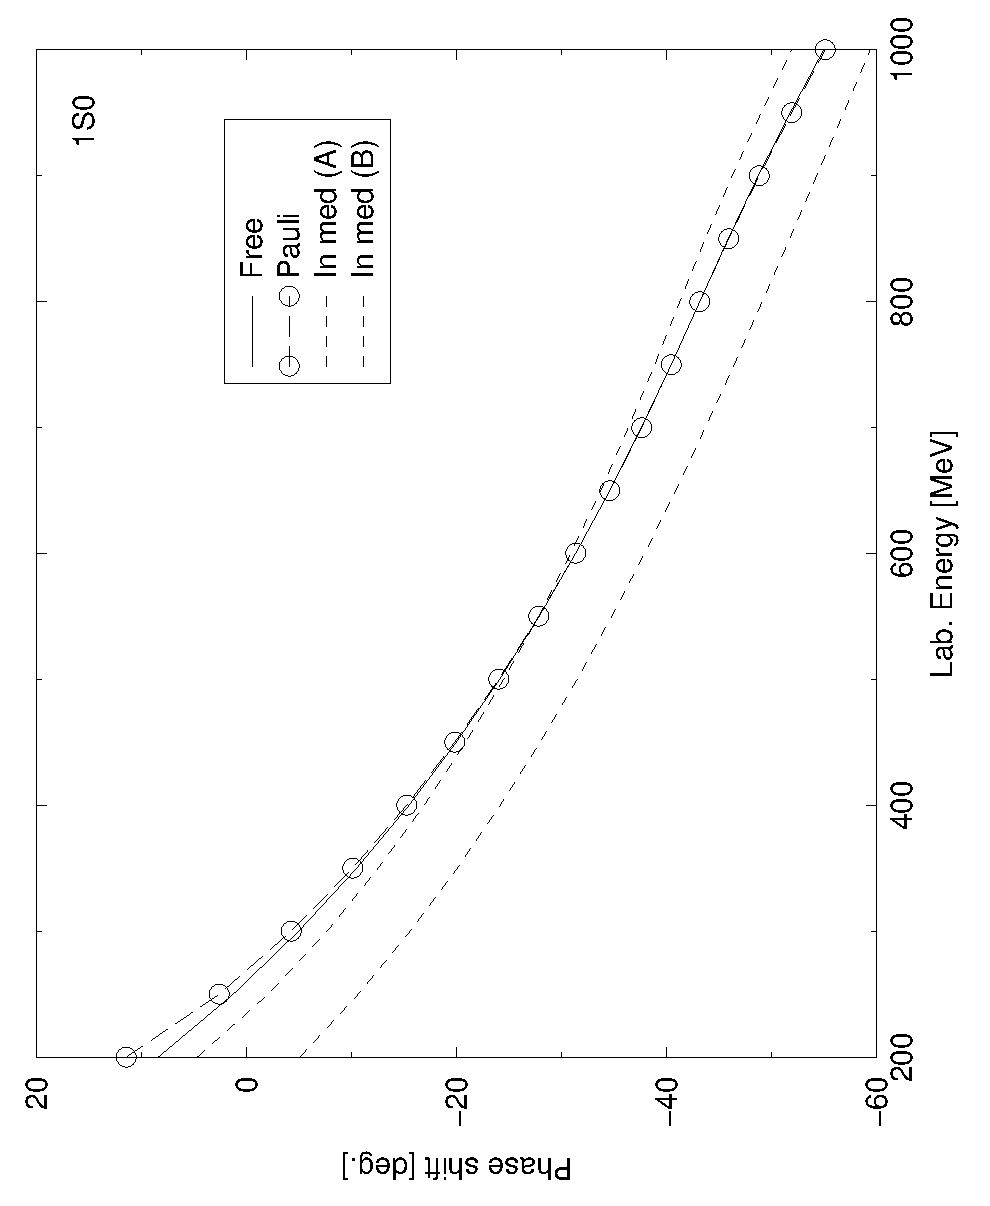
\includegraphics[height=7cm,width=7cm,angle=-90]{iii_elastinmedium.eps}
\qquad
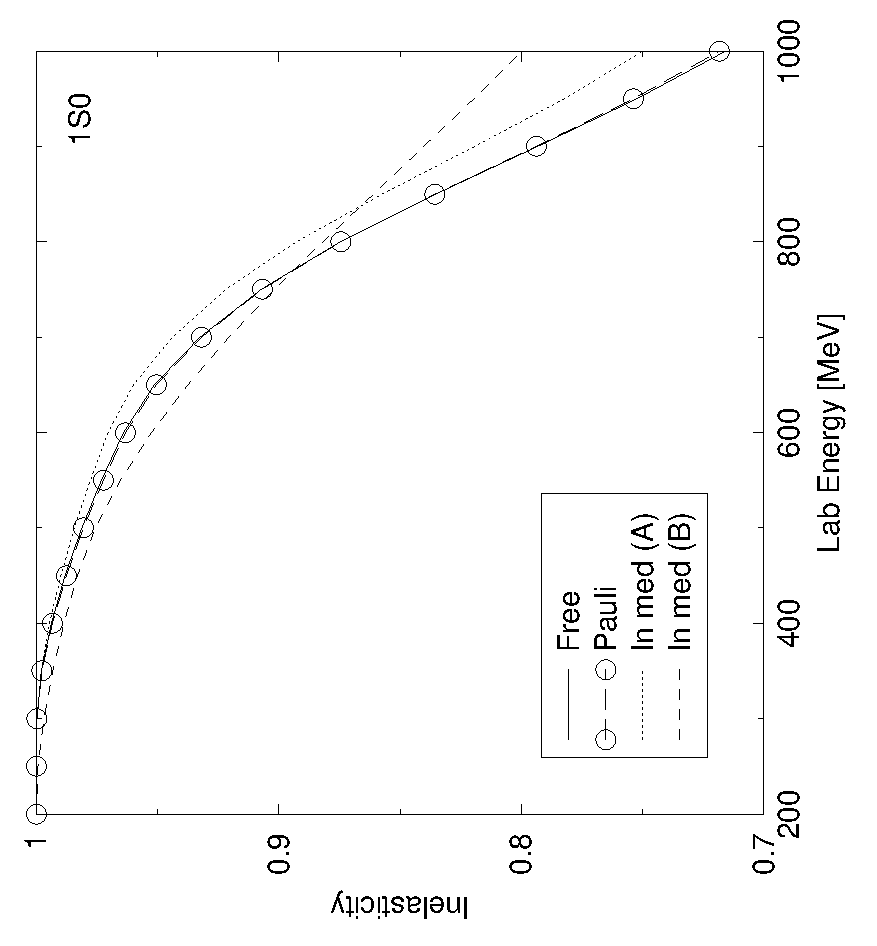
\includegraphics[height=7cm,width=7cm,angle=-90]{inelastinmedium.eps}
\caption{
\label{figInmediumphaseSandI}
Free and in-medium np scattering phase shifts and inelasticities for the partial \state{1}{S}{0}-state. 
as a function of of the incident energy. Where the free np scattering,
and three In-medium cross sections have been plotted. "Pauli" has only been included
the Pauli effect. "In med (A)" have only been included in-medium effects in the
$\LS$ equation. "In med (B)" has also been included the in-medium $\triangle$ effect. The results are obtained from 
the nna13 potential.
}
\end{figure}
\begin{figure}
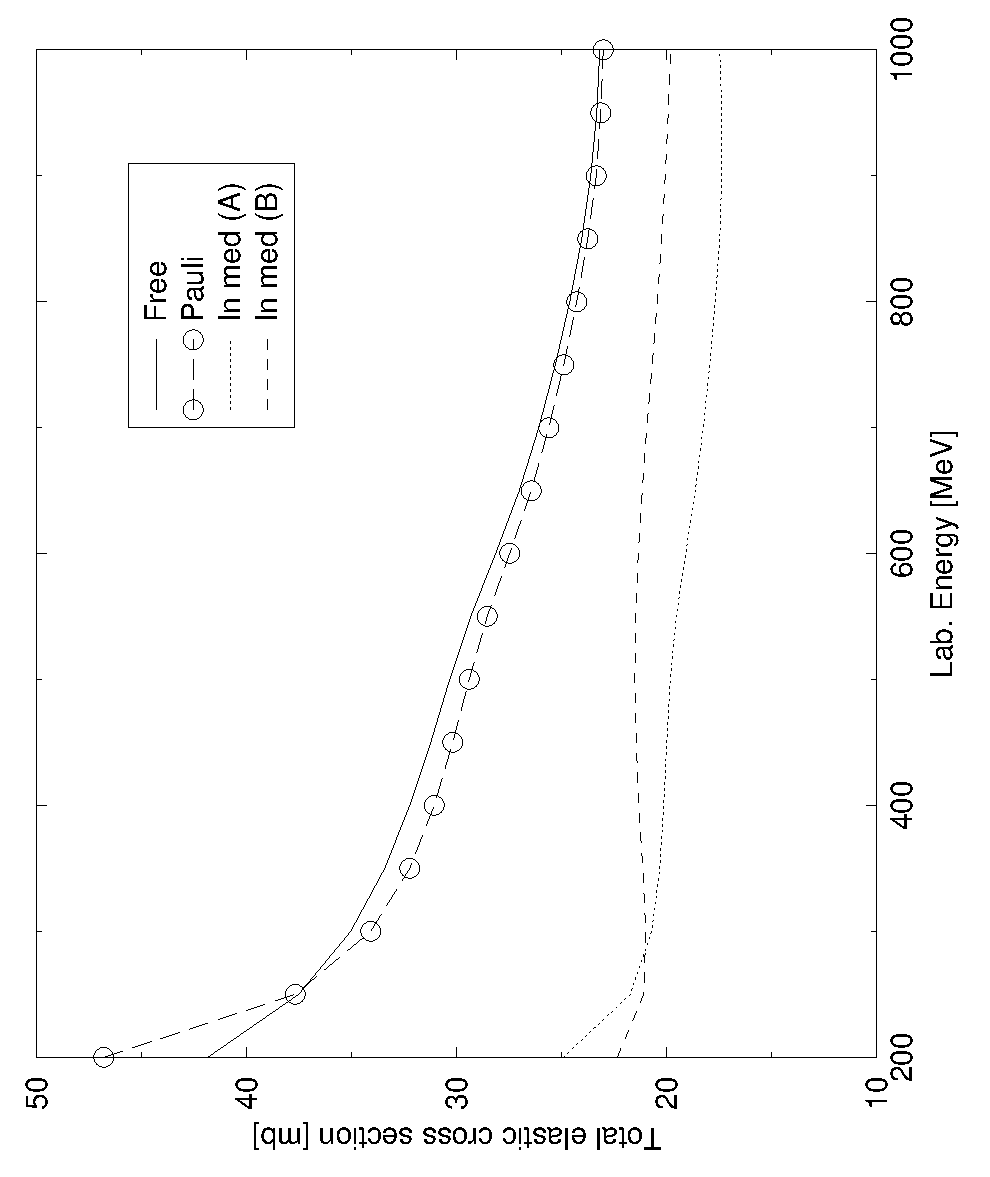
\includegraphics[height=7cm,width=7cm,angle=-90]{iii_crossPhaseS.eps}
\qquad
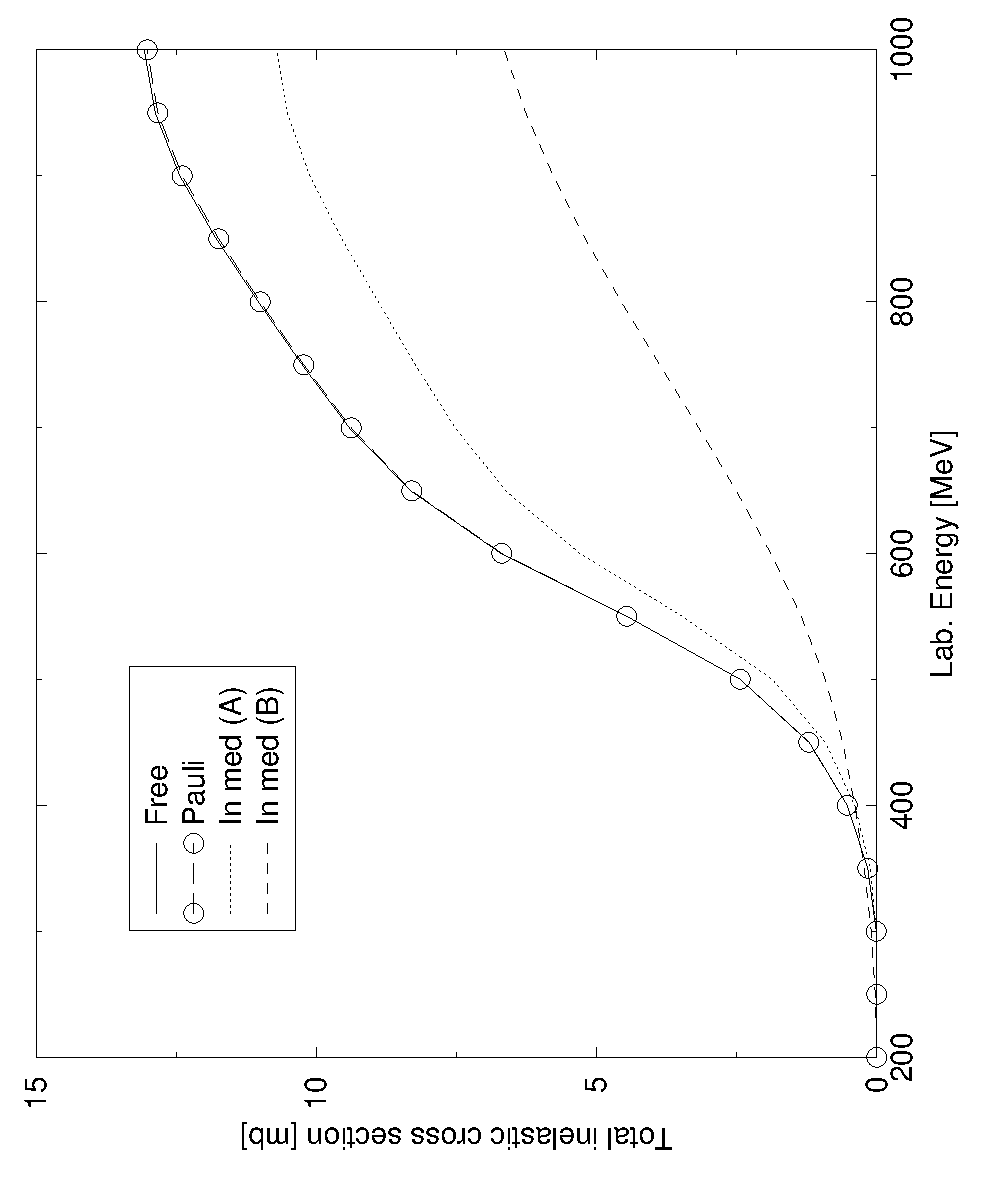
\includegraphics[height=7cm,width=7cm,angle=-90]{iii_crossInEl.eps}
\caption{
\label{figInmediumCrossS}
Free and in-medium np scattering cross sections.
Total cross sections for np scattering as a function of of the incident energy. Where the free np scattering,
and three In-medium cross sections have been plotted."Pauli" has only been included
the Pauli effect. "In med (A)" have only been included in-medium effects in the
$\LS$ equation. "In med (B)" has also been included the in-medium $\triangle$ effect. The results are obtained from
the nna13 potential.
}
\end{figure}

\documentclass[../main.tex]{subfiles}
 
\begin{document}

\begin{thebibliography}{99}

\bibitem{Manninen} S. M. Reimann and M. Manninen. Electronic structure of quantum dots. \emph{Reviews of Modern Physics}, \textbf{74}:1238, 2002. DOI: \url{https://doi.org/10.1103/RevModPhys.74.1283}.

\bibitem{QDotSolar} Z. Zheng, H. Ji, P. Yu and Z. Wang. Recent Progress Towards Quantum Dot Solar Cells with Enhanced Optical Absorption. \emph{Nanoscale Research Letters}, \textbf{11}:266, 2016. DOI: \url{https://doi.org/10.1186/s11671-016-1457-y}.

\bibitem{QDotSolar2} X. Lan, O. Voznyy, F. Pelayo García de Arquer, M. Liu, J. Xu, A. H. Proppe, G. Walters, F. Fan, H. Tan, M. Liu, Z. Yang, S. Hoogland, and E. H. Sargent. 10.6\% Certified Colloidal Quantum Dot Solar Cells via Solvent-Polarity-Engineered Halide Passivation. \emph{Nano Letters} \textbf{16}(7):4630-4634, 2016. DOI: \url{https://doi.org/10.1021/acs.nanolett.6b01957}.

\bibitem{QDotMed} S. Jin, Y. Hu, Z. Gu, L. Liu, and H. Wu. Application of Quantum Dots in Biological Imaging. \emph{Journal of Nanomaterials} \textbf{2011}:834139, 2011. DOI: \url{https://doi.org/10.1155/2011/834139}.

\bibitem{QDotMed2} L. A. Bentolila, X. Michalet, F. F. Pinaud, J. M. Tsay, S. Doose, J. J. Li, G. Sundaresan, A. M. Wu, S. S. Gambhir, S. Weiss. Quantum dots for molecular imaging and cancer medicine. \emph{Discovery Medicine} \textbf{5}(26):213–218, 2005. \url{https://www.ncbi.nlm.nih.gov/pubmed/20704913}

\bibitem{QDotLaser} N. N. Ledentsov. Quantum dot laser. \emph{Semiconductor Science and Technology} \textbf{26}:014001, 2011. DOI: \url{https://doi.org/10.1088/0268-1242/26/1/014001}.

\bibitem{QDotLaser2} V. H. Iyer, R. Mahadevu, and A. Pandey. Low Threshold Quantum Dot Lasers. \emph{The Journal of Physical Chemistry Letters} \textbf{7}(7):1244-1248, 2016. DOI: \url{https://doi.org/10.1021/acs.jpclett.6b00430}.

\bibitem{QDotComp} H. Wei and F. Deng. Scalable quantum computing based on stationary spin qubits in coupled quantum dots inside double-sided optical microcavities. \emph{Scientific Reports} \textbf{4}:7551, 2014. DOI: \url{https://doi.org/10.1038/srep07551}.

\bibitem{QDotComp2} M. A. Eriksson, M. Friesen, S. N. Coppersmith, R. Joynt, L. J. Klein, K. Slinker, C. Tahan, P. M. Mooney, J. O. Chu and S. J. Koester. Spin-Based Quantum Dot Quantum Computing in Silicon.\emph{Quantum Information Processing} \textbf{3}:133, 2004. DOI: \url{https://doi.org/10.1007/s11128-004-2224-z}.

\bibitem{QMC1} F. Bolton. Fixed-phase quantum Monte Carlo method applied to interacting electrons in
a quantum dot. \emph{Physical Review B} \textbf{54}:4780, 1996. DOI: \url{https://doi.org/10.1103/PhysRevB.54.4780}.

\bibitem{QMC2} F. Pederiva, C. J. Umrigar, and E. Lipparini. Diffusion Monte Carlo study of
circular quantum dots. \emph{Physical Review B} \textbf{62}:8120, 2000. DOI: \url{https://doi.org/10.1103/PhysRevB.62.8120}.

\bibitem{QMC3} A. D. Güçlü, Jian-Sheng Wang, and Hong Guo. Disordered quantum dots: A diffusion
quantum Monte Carlo study. \emph{Physical Review B} \textbf{68}:035304, 2003. DOI: \url{https://doi.org/10.1103/PhysRevB.68.035304}.

\bibitem{QDotBenchmarks} M.~.L.~Pedersen, G.~Hagen, M.~Hjorth-Jensen, S.~Kvaal, and F.~Pederiva. Ab initio computation of the energies of circular quantum dots. \emph{Physical Review B} {\bf 84}:115302, 2011. DOI: \url{https://doi.org/10.1103/PhysRevB.84.115302}.

\bibitem{ultra-cold neutrons} P. R. Huffman, C. R. Brome, J. S. Butterworth, K. J. Coakley, M. S. Dewey, S. N. Dzhosyuk, R. Golub, G. L. Greene, K. Habicht, S. K. Lamoreaux, C. E. H. Mattoni, D. N. McKinsey, F. E. Wietfeldt and J. M. Doyle. Magnetic trapping of neutrons. \emph{Nature} \textbf{403}:62-64, 2000. DOI: \url{https://doi.org/10.1038/47444}.
%Neutron Trapping Demonstrated for First Time at NIST. January 05, 2000. \url{https://www.nist.gov/news-events/news/2000/01/neutron-trapping-demonstrated-first-time-nist}, Read 29.05.2017.

\bibitem{Gardiner} C. W. Gardiner. \emph{Handbook of Stochastic Methods for Physics, Chemistry and the Natural Sciences}, Springer, 2nd edition, 1985.

\bibitem{Flyvbjerg} H. Flyvbjerg and H. G. Petersen. Error estimates on averages of correlated data. \emph{The Journal of Chemical Physics} \textbf{91}:461, 1989. DOI: \url{https://doi.org/10.1063/1.457480}.

%\bibitem{FYS4411-CG} M.~Hjorth-Jensen, {\em Conjugate gradient methods and other optimization methods},  \url{https://github.com/CompPhysics/ComputationalPhysics2/blob/master/doc/pub/cg/pdf/cg-print.pdf}, Read: 17.03.2016.

\bibitem{Kalos} J. W. Moskowitz, M. H. Kalos. A new look at correlations in atomic and molecular systems. I. Application of fermion monte carlo variational method. \emph{International Journal of Quantum Chemistry} \textbf{20}:1107, 1981. DOI: \url{https://doi.org/10.1002/qua.560200508}.

\bibitem{Taut} M.~Taut. Two electrons in an external oscillator potential: Particular analytic solutions
of a Coulomb correlation problem. \emph{Physical Review A} {\bf 48}:3561-3566, 1993. DOI: \url{https://doi.org/10.1103/PhysRevA.48.3561}.

%\bibitem{FYS4411-Slides} M.~Hjorth-Jensen, \emph{Computational Physics 2: Variational Monte Carlo methods}, \url{https://github.com/CompPhysics/ComputationalPhysics2/blob/master/doc/pub/vmc/pdf/vmc-print.pdf}, Read: 16.06.2016.

\bibitem{FYS4411-LectureNotes} M.~Hjorth-Jensen, \emph{Computational Physics Lecture Notes Fall 2015},  \url{https://github.com/CompPhysics/ComputationalPhysics2/blob/master/doc/Literature/lectures2015.pdf}.%, Chapter 16.10, Read: 16.06.2016.

\bibitem{Griffiths} D. J. Griffiths, \emph{Introduction to Quantum Mechanics}, Pearson,
2nd edition, 2005.

\bibitem{Scientific Computing} A. Tveito, H. P. Langtangen, B. F. Nielsen and X. Cai, \emph{Elements of Scientific Computing}, Springer, 1st edition, 2010.

\bibitem{Hermite} B.H. Bransden and C.J. Joachain, \emph{Physics of Atoms and molecules}, Longman, 1983. Chapter
2.

\bibitem{Schrodinger} Georgia State University, \emph{Time Independent Schrodinger Equation}, Hyperphysics entry, \url{http://hyperphysics.phy-astr.gsu.edu/hbase/quantum/Scheq.html}, Read 23.05.17.

%\bibitem{CP1_Project 2} M.~Hjorth-Jensen, \url{https://github.com/CompPhysics/ComputationalPhysics/blob/master/doc/Projects/2015/Project2/project2_2015.pdf}

\bibitem{master project} M.~Hjorth-Jensen. \url{https://github.com/CompPhysics/ThesisProjects/blob/master/doc/pub/quantumdots/pdf/quantumdots-minted.pdf}.

%\bibitem{basicMB} M.~Hjorth-Jensen, \emph{Hartree-Fock methods and introduction to Many-body Theory}, \url{https://github.com/CompPhysics/ComputationalPhysics2/blob/gh-pages/doc/pub/basicMB/pdf/basicMB-print.pdf}

\bibitem{Ruder} S. Ruder, An overview of gradient descent optimization
algorithms. \href{https://arxiv.org/abs/1609.04747}{arXiv:1609.04747 [cs.LG]}, 2016.

%\bibitem{QD-wiki} \url{https://en.wikipedia.org/wiki/Quantum_dot}, Read: 16.06.2016.

\bibitem{Stroustrup} B. Stroustrup, \emph{Bjarne Stroustrup's C++ Glossary}.  \url{http://www.stroustrup.com/glossary.html#Gpolymorphism}, Read: 09.05.2017.

\bibitem{gccDocs} \emph{Using the GNU Compiler Collection (GCC)}. section 3.10: Options That Control Optimization. \url{http://gcc.gnu.org/onlinedocs/gcc/Optimize-Options.html}, Read 10.05.2017.

\bibitem{github} Christian Fleishcer, Github Repository 2017,. \url{https://github.com/christianfleischer/Quantum-Dot-Project}.

\bibitem{Blaise} B. Barney. Lawrence Livermore National Laboratory. \emph{Introduction to Parallel Computing}. \url{https://computing.llnl.gov/tutorials/parallel_comp/}, Read 26.05.2017.

\bibitem{Wheeler} D. A. Wheeler. \emph{Secure Programming HOWTO}, Chapter 7.  \url{https://www.dwheeler.com/secure-programs/Secure-Programs-HOWTO/avoid-race.html}, Read 23.05.2017.

\bibitem{Lin} C. Lin. \emph{Logic Gates}. computer organization class notes, 2003. \url{https://www.cs.umd.edu/class/sum2003/cmsc311/Notes/Comb/gates.html}, Read 23.05.2017.

\bibitem{Yang} Y. M. Wang. Coupled-Cluster Studies of Double Quantum
Dots. Master’s thesis, University of Oslo, 2011. \url{http://urn.nb.no/URN:NBN:no-28527}.

\bibitem{Jorgen} J. Høgberget. Quantum Monte-Carlo Studies of Generalized Many-body Systems. 
Master’s thesis, University of Oslo, 2013. \url{http://urn.nb.no/URN:NBN:no-38645}.

\bibitem{Reimann} S. Reimann. Quantum-mechanical systems in traps and Similarity Renormalization Group theory. Master’s thesis, University of Oslo, 2013. \url{http://urn.nb.no/URN:NBN:no-38639}.

\bibitem{Hirth} C. Hirth. Studies of quantum dots: Ab initio coupledcluster analysis using OpenCL and GPU programming. Master’s thesis, University of Oslo, 2012. \url{http://urn.nb.no/URN:NBN:no-31657}.

\bibitem{Olsen} V. K. B. Olsen. Full Configuration Interaction Simulation of Quantum Dots. Master’s thesis, University of Oslo, 2012. \url{http://urn.nb.no/URN:NBN:no-32952}.

\bibitem{Armadillo} C. Sanderson and R. Curtin. Armadillo: a template-based C++ library for linear algebra. 
\emph{Journal of Open Source Software} \textbf{1}:26, 2016. \url{http://dx.doi.org/10.21105/joss.00026}.

\bibitem{Open MPI} E. Gabriel, G. E. Fagg, G. Bosilca, T. Angskun, J. J. Dongarra, J. M. Squyres, V. Sahay, P. Kambadur, B. Barrett, A. Lumsdaine, R. H. Castain, D. J. Daniel, R. L. Graham, and T. S. Woodall. Open MPI: Goals, Concept, and Design of a Next Generation MPI Implementation. In Proceedings, 11th European PVM/MPI Users' Group Meeting, Budapest, Hungary, September 2004.

\bibitem{Matplotlib} J. D. Hunter. Matplotlib: A 2D Graphics Environment. \emph{Computing in Science \& Engineering} \textbf{9}:90-95, 2007. DOI: \url{http://dx.doi.org/10.1109/MCSE.2007.55}, Publisher link: \url{http://aip.scitation.org/doi/abs/10.1109/MCSE.2007.55}.

\bibitem{NumPy} S. van der Walt, S. C. Colbert and G. Varoquaux. The NumPy Array: A Structure for Efficient Numerical Computation. \emph{Computing in Science \& Engineering} \textbf{13}:22-30, 2011.  DOI: \url{http://dx.doi.org/10.1109/MCSE.2011.37}, Publisher link: \url{http://aip.scitation.org/doi/abs/10.1109/MCSE.2011.37}.

\bibitem{SymPy} A. Meurer, C. P. Smith, M. Paprocki, O. Čertík, S. B. Kirpichev, M. Rocklin, A. Kumar, S. Ivanov, J. K. Moore, S. Singh, T. Rathnayake, S. Vig, B. E. Granger, R. P. Muller, F. Bonazzi, H. Gupta, S. Vats, F. Johansson, F. Pedregosa, M. J. Curry, A. R. Terrel, Š. Roučka, A. Saboo, I. Fernando, S. Kulal, R. Cimrman, A. Scopatz. SymPy: symbolic computing in Python. \emph{PeerJ Computer Science} \textbf{3}:e103, 2017. DOI: \url{https://doi.org/10.7717/peerj-cs.103}.

\bibitem{Multiwells} D. V. Schroeder, \emph{Multiple Wells} \url{http://physics.weber.edu/schroeder/quantum/MultipleWells.pdf}, Read 26.05.2017.



\end{thebibliography}
\end{document}
%\bibliography{ref.bib}


%\include{egenteori4}



% \pagestyle{empty}
% \include{framsida}
 %\cleardoublepage
 %\include{fystesia}
% \cleardoublepage
% \include{forord} %%\section*{Forord}

 %\begin{flushleft}
% \tableofcontents
% \pagestyle{myheadings}
% \thispagestyle{empty}
 %\end{flushleft}
% \cleardoublepage 

% \kap{Introduction}\label{chap:innledning}
%\begin{flushleft}


\section[Nucleon-Nucleon models]{Nucleon-Nucleon(NN) interactions And Nuclear Models}



Particles can be grouped into three different categories, which are leptons, baryons and mesons.
Leptons are particles like the electron and neutrino. 
Baryons are particles with half integer spin like the nucleons,
while mesons are particles with integer spin.
It is also normal to call the big group of baryons and mesons for hadrons, since they are all made from quarks.

The mesons are the carrier of the strong force. They can interact with nucleons through the strong, weak,
electromagnetic and gravitational force. Free mesons can be produced in nucleon-nucleon collisions, but they decay
rapidly into lighter mesons, leptons or photons either through strong, weak or electromagnetic interactions. 
The decay lifetimes are around $10^{-20}-10^{-23}$ for strong decays, $10^{-16}-10^{-18}$ for electromagnetic decays 
and $10^{-8}-10^{-10}$ for weak decay. In the nucleon-nucleon scattering processes we are looking at, we can
neglect all the other forces except the strong force. So the contribution to the potential created between
the nucleons are  only arising from strong interactions through virtual meson exchange.

There are many different mesons. They all have their own contribution to the strong force,
which is a superposition from all the possible ways the mesons can be exchanged. 
i.e. not only a single meson exchange, but also more complicated events where two ore more mesons are transfered.
All the mesons have their own characteristic combination of mass, spin, parity, isospin and decay rate. 
these parameters are important for the range of the force, but also for where it will be repulsive/attractive.
It is normal to divide the range of the strong force into three regions; 
The short range, the intermediate region and the long-range of the force.
For example the $\pi$-meson as the lightest particle provides the long-range force. 
While the $\omega$-meson is responsible for the short-range repulsion, which explains the observed hard core of
the nucleons when they are squeezed together. From electron scattering experiments on heavy nuclears,
one have found an average distance between the centers of the nucleons to be 1.8 fm. 
This is a too large diameter of the hard core arising from the strong force. It turns out that the Pauli 
principal is more important for nucleons hard core observed in heavy nuclears. 
A better way to determine the hard core from the strong interaction is NN data form the \state{1}{S}{0}- phase shift.
This state is chosen since it doesn't have a centrifugal barrier. i.e. the angular orbital momentum; L=0. 
From fig~\ref{fig:manypotS} we see that the phase shift turns negative/repulsive around $E_{lab}=250$ MeV.
The maximum classical orbital angular momentum $L_{max}$ is
\begin{equation}\label{eq:Lmax}
L_{max}=Rp=R\sqrt{\frac{E_{lab}M}{2}}
\end{equation}
Where R is the range/radius of the hard core and M is the mass of the nucleon.
With $L\le1$ we obtain an estimate of the radius of the hard core: 
\begin{equation}\label{eq:Lmax2}
R\le 0.6 \text{ fm}
\end{equation}
Experiments shows that the deuterium has a magnetic moment, which means that the bound nuclei is a mixture
of the S-state (L=0) and the D-state (L=2). This indicates that the strong force also contains a tensor-force
that can couple the two states with the same good quantum numbers. 
%This indicates that we need more than 
%the Klein-Gordon equation, which is the relativistic wave equation for scalar fields. 
The Klein-Gordon equation is used to calculate a potential from mesons with spin-$0$ (Yukawa potentials).
The Yukawa potential has it origin from a scalar-force.
This indicates that we need to work with more than
the Klein-Gordon equation to reproduce the tensor-force.
%, which is the relativistic wave equation for scalar fields.
The Dirac equation on the other hand will be able of handling tensor-forces, 
but is only valid for half integer spin particles like nucleons and quarks.
One must of course use field theories for spin-1, spin-2 and higher spin models.
Spin-1 theory for meson has much in common with the field theory for photons. 
Photons also have spin-1, but unlike the mesons, it has zero mass. 
It turns out that spin-1 fields can create a tensor force.
Models for the higher spin-mesons exist, but
One Boson Exchange (OBE) models, like the Bonn B potential, normally only include spin-0 and spin-1 mesons.
This approximation is good because the mesons are generally heavier as the spin increases.
The heavier mesons will only have a short range. Their contribution will be small to the strong force.
In Bonn B for example the $\sigma$-meson are supposed to be the average effect of all the heavier mesons and all the
multiple meson exchanges.
%So for the 
%Spin-1 field theories
%From definition the mesons are particles with integer spin.

%So to make a good potential of the strong interactions, one have to have in mind that mesons are made up of quarks
%with half integer spin. One also sees that the Klein Gordon equation no longer can be interpreted as a consistent
%one particle equation. 


All integer spin particles are made up of half integer spin particles. 
Handling the mesons as a particle will only give approximate theories to the real jungle.
This approximation gets worse and worse as the energy of the NN-system is increased. 
Finally the meson theory breaks down, and the system has to be dealt with as a system of quarks instead.
In OBE-models this effect is implemented as so called cutoff-parameters.

It is the strong force that holds the nucleons together in nuclears, but the Pauli principal is 
also important for the way nucleons binds and forms nuclears. 
From the decay rate we see that a meson can move a 
couple of Fermi meters before it decays through the strong force. This must off course hold for virtual mesons to. 
It is a relatively short 
range. So in a nuclear the strong force is (approximately) only active among neighboring nucleons. 
This explains why the binding energy per nucleon increases from the smallest nuclear ${}^2$H ($\sim$ 1 MeV) till 
${}^4$He ($\sim$ 7 MeV), 
and then is more stabile for larger nucleons. With a maximum at ${}^{56}$Fe ($\sim$ 8.5 MeV). 
The energy per bound is also interesting to look at.
The energy per bound is about 2 MeV for ${}^2$H, 3 MeV for the triton and 4.5 MeV for ${}^4$He. 
One can also conclude that; When nucleons are pulled closer to each other by more bonds due to more nucleons, 
but also the energy per bound increases to. This is an interesting effect created by a three body-force, which
has no classical analog.


This gives rise to different nuclear models like the liquid-drop model. 
The liquid-drop model has only the protons and the total number of nucleons as parameters.
A much better model would of course be to use the exact potential that is created through meson exchange,
and then build up the nuclears with it.
In order to do that, the first thing one needs is a model of the potential. This has led to a own branch in
nuclear physics.

Calculating the phase shifts gives an indication of the strength of the potential between the two nucleons.
If one has a good guess of how the potential must be, one can test it by running a computer program 
(like one described later) to calculate the phase shift and inelasticity. 
One can in principal check the theoretical potential with experimental values of phase shift and inelasticity,
which we now have very good experimental values for.
The One Boson Exchange (OBE)-model is such a theoretical potential.
As mentioned before, this potential contains a couple of "cutoff" parameters and a fictive $\sigma$-meson, 
which has to be adjusted to fit the experimental values as good as possible. This model gets very close to
the experimental data for low energies. But it is a little bit too steep in many cases, like it is in 
fig~\ref{fig:manypotS}. New and better models have been developed the recent years.
Charge-Dependent (CD) Bonn is one of them ~\cite{cd-bonn}. 
This model is building on the OBE model but is using charge dependents, i.e. u and d quarks has different masses.
This model can reproduce almost exact results for lab energies below 300 MeV, 
when it is fitted with experimental data. This is a good indication of the isospin dependence of the strong force,
and indicates that the meson-theory is good. It is actually so good that Machleidt, my supervisor here in USA 
who worked on the CD-Bonn potential, has focused his interest in solving the higher energy models instead. 
These models has to account on more complex meson exchanges, excitations of the nucleons, 
and even production of other particles.
The new high energy models also include properties taken from quantum chromodynamics (QCD).
%The next step for these models seems to be
Like confinement and chiral perturbation, which seems to be the next step in modeling the strong force.

The meson theory has been developed from a wish to understand the basic force holding the nucleons together. 
When the meson-model work well compared with it's limited accuracy, one will have to try to solve the "real" problem. 
i.e. leaving the mesons and nucleon, which is a sort of an approximation of how the quarks behavior.
Such quark models are still far from being good, but hopefully it will be worked out one day. 

%The next step now seems to be confinement and chiral
%perturbation models, which is mostly  the old meson theory, but includes properties of quantum chromodynamics (QCD). 

The meson model has been polished for quite a time now, and is the best model we have of
the strong interaction.
But even with a good potential model of the strong force, it is difficult to apply it to nuclears. 
The strong force is a three body force. That is, the force on nucleon 1 not only depends on the individual
position of nucleon 2 and 3, it contains an additional contribution that arises from the correlation 
of the positions of nucleon 2 and 3. 
Solving this problem exact is difficult for heavy nuclears since it is dependent on all the nucleons position in the nuclear.
The mathematic is complicated and one loose physical insight.

People have compared this model with describing a gas by how all the molecule move, rather than using a few parameters such as 
pressure and temperature. They want to use oversimplified theories like  "shell models" to describe nuclears. 
This theory is mathematically easy to work with and gives a good physical insight. 
One can for example see from this theory that the strong interaction must include a spin-orbit force and a
spin-spin ($\sigma\cdot\sigma$) force. But these forces can also be studied in 
NN-scattering. For example can the spin-orbit
force be observed in pp-scattering experiments with the triplet P waves. 

The nuclear science has been divided by different models.
This way the theoretical nuclear group in Oslo and Bergen have ended up working with two different theories even though 
they work with the exact same problem.  

\section{Phase Shift For Partial Waves} 

As mentioned already, phase shifts are very important for the understanding of the strong force.
Phase shift $\delta_l$ is a result from the de Broglies postulate, which states that particles also behaves as waves.
Particles have  a wave length $\lambda$, called de Broglie wavelength related to the particle's momentum p as
\begin{equation}\label{eq:Broglie}
\lambda=\frac{2\pi\hbar}{p}
\end{equation}
$\lambda$ will therefor be dependent on the energy of the particle/(wave packet). This is illustrated
in fig~\ref{fig:ilusterendeFaseskift}. Note that $\lambda$=$\pi\delta$, where $\delta$ is the phase shift.
\begin{flushleft}   
\begin{figure}\label{fig:ilusterendeFaseskift}
\centering
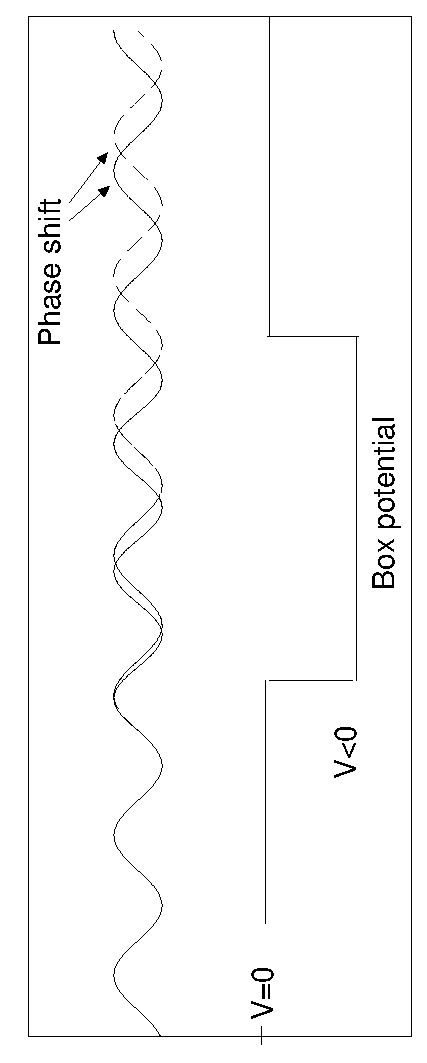
\includegraphics[height=15cm,angle=-90]{detteerfaseskift.eps}
\caption{Shows how a wave function will behave for a attractive box potential. The dashed line
illustrates the wave function behavior with out the potential.}
\end{figure}
\end{flushleft} 
However the phase shift can not be found directly. Experimentalist have to study the observable, 
which can be for example differential cross section and polarization. With these data, theorists are
able to calculate an NN-amplitude (A) for the process. This amplitude has many of the same properties as the S-matrix,
like the unitarian. In partial wave decomposition, it is related to the phase shift $\delta_l$ as
\begin{equation}
A_l=\eta_l e^{i2\delta_l}
\end{equation}

Inelasticity ($\eta_l$) is the probability amplitude for the scattering amplitude to be elastic. 
The inelasticity and phase shift are the necessary parameters to describe a partial wave. The inelasticity
becomes important for NN-scattering when the kinetic energy in the lab-system are above 350 MeV.
The inelasticity are due to energy released from the NN-system. This can be done by photon emission and/or particle
creations in the scattering.

  
%fig~\ref{fig:manypotS} shows the phase shift for different potentials and experimental phase shift.
%How the potentials are build up will be explained later.



\begin{flushleft} 

\begin{figure}\label{fig:manypotS}
\centering
\includegraphics[height=17cm]{manypotS.eps} 
\caption{\state{1}{S}{0} phase shifts for a box Potential, a parameterized potential, the Bonn B potential and
experimental data ~\cite{PRC48faseskift350MeV}. How the potentials are build up will be explained later.}
\end{figure}


\end{flushleft}



% \include{femstore}
 %\include{bramatriser} %\include{matriser}
% \include{kaluzaklein} %\include{kap2m}
% \include{jordan}
% \include{kosmologi}
% \include{skalar} %\include{kos44}
% \include{gaugecas} %\include{casimir}
% \include{topot}
% \include{konk}

\appendix
%\kap{Introduction}\label{chap:innledning}
%\begin{flushleft}


\section[Nucleon-Nucleon models]{Nucleon-Nucleon(NN) interactions And Nuclear Models}



Particles can be grouped into three different categories, which are leptons, baryons and mesons.
Leptons are particles like the electron and neutrino. 
Baryons are particles with half integer spin like the nucleons,
while mesons are particles with integer spin.
It is also normal to call the big group of baryons and mesons for hadrons, since they are all made from quarks.

The mesons are the carrier of the strong force. They can interact with nucleons through the strong, weak,
electromagnetic and gravitational force. Free mesons can be produced in nucleon-nucleon collisions, but they decay
rapidly into lighter mesons, leptons or photons either through strong, weak or electromagnetic interactions. 
The decay lifetimes are around $10^{-20}-10^{-23}$ for strong decays, $10^{-16}-10^{-18}$ for electromagnetic decays 
and $10^{-8}-10^{-10}$ for weak decay. In the nucleon-nucleon scattering processes we are looking at, we can
neglect all the other forces except the strong force. So the contribution to the potential created between
the nucleons are  only arising from strong interactions through virtual meson exchange.

There are many different mesons. They all have their own contribution to the strong force,
which is a superposition from all the possible ways the mesons can be exchanged. 
i.e. not only a single meson exchange, but also more complicated events where two ore more mesons are transfered.
All the mesons have their own characteristic combination of mass, spin, parity, isospin and decay rate. 
these parameters are important for the range of the force, but also for where it will be repulsive/attractive.
It is normal to divide the range of the strong force into three regions; 
The short range, the intermediate region and the long-range of the force.
For example the $\pi$-meson as the lightest particle provides the long-range force. 
While the $\omega$-meson is responsible for the short-range repulsion, which explains the observed hard core of
the nucleons when they are squeezed together. From electron scattering experiments on heavy nuclears,
one have found an average distance between the centers of the nucleons to be 1.8 fm. 
This is a too large diameter of the hard core arising from the strong force. It turns out that the Pauli 
principal is more important for nucleons hard core observed in heavy nuclears. 
A better way to determine the hard core from the strong interaction is NN data form the \state{1}{S}{0}- phase shift.
This state is chosen since it doesn't have a centrifugal barrier. i.e. the angular orbital momentum; L=0. 
From fig~\ref{fig:manypotS} we see that the phase shift turns negative/repulsive around $E_{lab}=250$ MeV.
The maximum classical orbital angular momentum $L_{max}$ is
\begin{equation}\label{eq:Lmax}
L_{max}=Rp=R\sqrt{\frac{E_{lab}M}{2}}
\end{equation}
Where R is the range/radius of the hard core and M is the mass of the nucleon.
With $L\le1$ we obtain an estimate of the radius of the hard core: 
\begin{equation}\label{eq:Lmax2}
R\le 0.6 \text{ fm}
\end{equation}
Experiments shows that the deuterium has a magnetic moment, which means that the bound nuclei is a mixture
of the S-state (L=0) and the D-state (L=2). This indicates that the strong force also contains a tensor-force
that can couple the two states with the same good quantum numbers. 
%This indicates that we need more than 
%the Klein-Gordon equation, which is the relativistic wave equation for scalar fields. 
The Klein-Gordon equation is used to calculate a potential from mesons with spin-$0$ (Yukawa potentials).
The Yukawa potential has it origin from a scalar-force.
This indicates that we need to work with more than
the Klein-Gordon equation to reproduce the tensor-force.
%, which is the relativistic wave equation for scalar fields.
The Dirac equation on the other hand will be able of handling tensor-forces, 
but is only valid for half integer spin particles like nucleons and quarks.
One must of course use field theories for spin-1, spin-2 and higher spin models.
Spin-1 theory for meson has much in common with the field theory for photons. 
Photons also have spin-1, but unlike the mesons, it has zero mass. 
It turns out that spin-1 fields can create a tensor force.
Models for the higher spin-mesons exist, but
One Boson Exchange (OBE) models, like the Bonn B potential, normally only include spin-0 and spin-1 mesons.
This approximation is good because the mesons are generally heavier as the spin increases.
The heavier mesons will only have a short range. Their contribution will be small to the strong force.
In Bonn B for example the $\sigma$-meson are supposed to be the average effect of all the heavier mesons and all the
multiple meson exchanges.
%So for the 
%Spin-1 field theories
%From definition the mesons are particles with integer spin.

%So to make a good potential of the strong interactions, one have to have in mind that mesons are made up of quarks
%with half integer spin. One also sees that the Klein Gordon equation no longer can be interpreted as a consistent
%one particle equation. 


All integer spin particles are made up of half integer spin particles. 
Handling the mesons as a particle will only give approximate theories to the real jungle.
This approximation gets worse and worse as the energy of the NN-system is increased. 
Finally the meson theory breaks down, and the system has to be dealt with as a system of quarks instead.
In OBE-models this effect is implemented as so called cutoff-parameters.

It is the strong force that holds the nucleons together in nuclears, but the Pauli principal is 
also important for the way nucleons binds and forms nuclears. 
From the decay rate we see that a meson can move a 
couple of Fermi meters before it decays through the strong force. This must off course hold for virtual mesons to. 
It is a relatively short 
range. So in a nuclear the strong force is (approximately) only active among neighboring nucleons. 
This explains why the binding energy per nucleon increases from the smallest nuclear ${}^2$H ($\sim$ 1 MeV) till 
${}^4$He ($\sim$ 7 MeV), 
and then is more stabile for larger nucleons. With a maximum at ${}^{56}$Fe ($\sim$ 8.5 MeV). 
The energy per bound is also interesting to look at.
The energy per bound is about 2 MeV for ${}^2$H, 3 MeV for the triton and 4.5 MeV for ${}^4$He. 
One can also conclude that; When nucleons are pulled closer to each other by more bonds due to more nucleons, 
but also the energy per bound increases to. This is an interesting effect created by a three body-force, which
has no classical analog.


This gives rise to different nuclear models like the liquid-drop model. 
The liquid-drop model has only the protons and the total number of nucleons as parameters.
A much better model would of course be to use the exact potential that is created through meson exchange,
and then build up the nuclears with it.
In order to do that, the first thing one needs is a model of the potential. This has led to a own branch in
nuclear physics.

Calculating the phase shifts gives an indication of the strength of the potential between the two nucleons.
If one has a good guess of how the potential must be, one can test it by running a computer program 
(like one described later) to calculate the phase shift and inelasticity. 
One can in principal check the theoretical potential with experimental values of phase shift and inelasticity,
which we now have very good experimental values for.
The One Boson Exchange (OBE)-model is such a theoretical potential.
As mentioned before, this potential contains a couple of "cutoff" parameters and a fictive $\sigma$-meson, 
which has to be adjusted to fit the experimental values as good as possible. This model gets very close to
the experimental data for low energies. But it is a little bit too steep in many cases, like it is in 
fig~\ref{fig:manypotS}. New and better models have been developed the recent years.
Charge-Dependent (CD) Bonn is one of them ~\cite{cd-bonn}. 
This model is building on the OBE model but is using charge dependents, i.e. u and d quarks has different masses.
This model can reproduce almost exact results for lab energies below 300 MeV, 
when it is fitted with experimental data. This is a good indication of the isospin dependence of the strong force,
and indicates that the meson-theory is good. It is actually so good that Machleidt, my supervisor here in USA 
who worked on the CD-Bonn potential, has focused his interest in solving the higher energy models instead. 
These models has to account on more complex meson exchanges, excitations of the nucleons, 
and even production of other particles.
The new high energy models also include properties taken from quantum chromodynamics (QCD).
%The next step for these models seems to be
Like confinement and chiral perturbation, which seems to be the next step in modeling the strong force.

The meson theory has been developed from a wish to understand the basic force holding the nucleons together. 
When the meson-model work well compared with it's limited accuracy, one will have to try to solve the "real" problem. 
i.e. leaving the mesons and nucleon, which is a sort of an approximation of how the quarks behavior.
Such quark models are still far from being good, but hopefully it will be worked out one day. 

%The next step now seems to be confinement and chiral
%perturbation models, which is mostly  the old meson theory, but includes properties of quantum chromodynamics (QCD). 

The meson model has been polished for quite a time now, and is the best model we have of
the strong interaction.
But even with a good potential model of the strong force, it is difficult to apply it to nuclears. 
The strong force is a three body force. That is, the force on nucleon 1 not only depends on the individual
position of nucleon 2 and 3, it contains an additional contribution that arises from the correlation 
of the positions of nucleon 2 and 3. 
Solving this problem exact is difficult for heavy nuclears since it is dependent on all the nucleons position in the nuclear.
The mathematic is complicated and one loose physical insight.

People have compared this model with describing a gas by how all the molecule move, rather than using a few parameters such as 
pressure and temperature. They want to use oversimplified theories like  "shell models" to describe nuclears. 
This theory is mathematically easy to work with and gives a good physical insight. 
One can for example see from this theory that the strong interaction must include a spin-orbit force and a
spin-spin ($\sigma\cdot\sigma$) force. But these forces can also be studied in 
NN-scattering. For example can the spin-orbit
force be observed in pp-scattering experiments with the triplet P waves. 

The nuclear science has been divided by different models.
This way the theoretical nuclear group in Oslo and Bergen have ended up working with two different theories even though 
they work with the exact same problem.  

\section{Phase Shift For Partial Waves} 

As mentioned already, phase shifts are very important for the understanding of the strong force.
Phase shift $\delta_l$ is a result from the de Broglies postulate, which states that particles also behaves as waves.
Particles have  a wave length $\lambda$, called de Broglie wavelength related to the particle's momentum p as
\begin{equation}\label{eq:Broglie}
\lambda=\frac{2\pi\hbar}{p}
\end{equation}
$\lambda$ will therefor be dependent on the energy of the particle/(wave packet). This is illustrated
in fig~\ref{fig:ilusterendeFaseskift}. Note that $\lambda$=$\pi\delta$, where $\delta$ is the phase shift.
\begin{flushleft}   
\begin{figure}\label{fig:ilusterendeFaseskift}
\centering
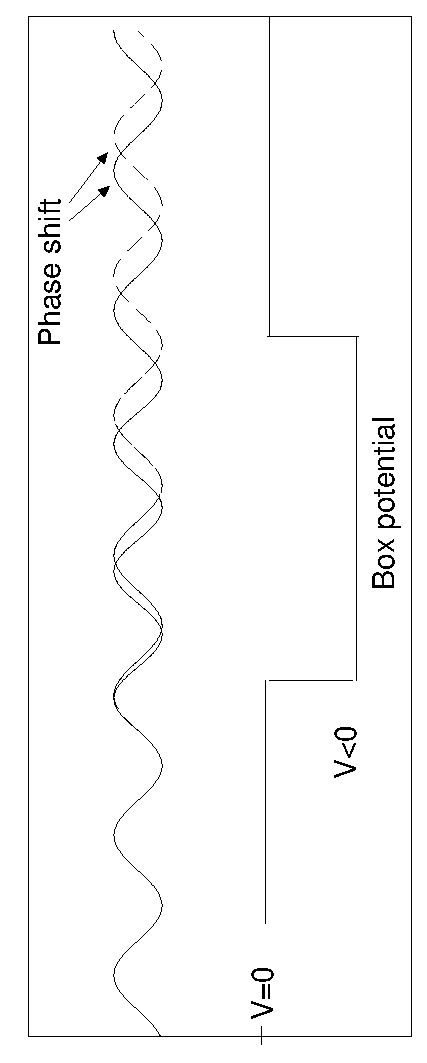
\includegraphics[height=15cm,angle=-90]{detteerfaseskift.eps}
\caption{Shows how a wave function will behave for a attractive box potential. The dashed line
illustrates the wave function behavior with out the potential.}
\end{figure}
\end{flushleft} 
However the phase shift can not be found directly. Experimentalist have to study the observable, 
which can be for example differential cross section and polarization. With these data, theorists are
able to calculate an NN-amplitude (A) for the process. This amplitude has many of the same properties as the S-matrix,
like the unitarian. In partial wave decomposition, it is related to the phase shift $\delta_l$ as
\begin{equation}
A_l=\eta_l e^{i2\delta_l}
\end{equation}

Inelasticity ($\eta_l$) is the probability amplitude for the scattering amplitude to be elastic. 
The inelasticity and phase shift are the necessary parameters to describe a partial wave. The inelasticity
becomes important for NN-scattering when the kinetic energy in the lab-system are above 350 MeV.
The inelasticity are due to energy released from the NN-system. This can be done by photon emission and/or particle
creations in the scattering.

  
%fig~\ref{fig:manypotS} shows the phase shift for different potentials and experimental phase shift.
%How the potentials are build up will be explained later.



\begin{flushleft} 

\begin{figure}\label{fig:manypotS}
\centering
\includegraphics[height=17cm]{manypotS.eps} 
\caption{\state{1}{S}{0} phase shifts for a box Potential, a parameterized potential, the Bonn B potential and
experimental data ~\cite{PRC48faseskift350MeV}. How the potentials are build up will be explained later.}
\end{figure}


\end{flushleft}



 %%%%%%%%%%%\include{maplepro}
% \include{mprog}

% \nocite{*}
 %\bibliographystyle{abbrv.bst}
 %\bibliographystyle{unsrt}
 %\begin{flushleft}
 %%%%%\headinga{Bibliografi}{}
% \bibliographystyle{plain} 
% \kap{Introduction}\label{chap:innledning}
%\begin{flushleft}


\section[Nucleon-Nucleon models]{Nucleon-Nucleon(NN) interactions And Nuclear Models}



Particles can be grouped into three different categories, which are leptons, baryons and mesons.
Leptons are particles like the electron and neutrino. 
Baryons are particles with half integer spin like the nucleons,
while mesons are particles with integer spin.
It is also normal to call the big group of baryons and mesons for hadrons, since they are all made from quarks.

The mesons are the carrier of the strong force. They can interact with nucleons through the strong, weak,
electromagnetic and gravitational force. Free mesons can be produced in nucleon-nucleon collisions, but they decay
rapidly into lighter mesons, leptons or photons either through strong, weak or electromagnetic interactions. 
The decay lifetimes are around $10^{-20}-10^{-23}$ for strong decays, $10^{-16}-10^{-18}$ for electromagnetic decays 
and $10^{-8}-10^{-10}$ for weak decay. In the nucleon-nucleon scattering processes we are looking at, we can
neglect all the other forces except the strong force. So the contribution to the potential created between
the nucleons are  only arising from strong interactions through virtual meson exchange.

There are many different mesons. They all have their own contribution to the strong force,
which is a superposition from all the possible ways the mesons can be exchanged. 
i.e. not only a single meson exchange, but also more complicated events where two ore more mesons are transfered.
All the mesons have their own characteristic combination of mass, spin, parity, isospin and decay rate. 
these parameters are important for the range of the force, but also for where it will be repulsive/attractive.
It is normal to divide the range of the strong force into three regions; 
The short range, the intermediate region and the long-range of the force.
For example the $\pi$-meson as the lightest particle provides the long-range force. 
While the $\omega$-meson is responsible for the short-range repulsion, which explains the observed hard core of
the nucleons when they are squeezed together. From electron scattering experiments on heavy nuclears,
one have found an average distance between the centers of the nucleons to be 1.8 fm. 
This is a too large diameter of the hard core arising from the strong force. It turns out that the Pauli 
principal is more important for nucleons hard core observed in heavy nuclears. 
A better way to determine the hard core from the strong interaction is NN data form the \state{1}{S}{0}- phase shift.
This state is chosen since it doesn't have a centrifugal barrier. i.e. the angular orbital momentum; L=0. 
From fig~\ref{fig:manypotS} we see that the phase shift turns negative/repulsive around $E_{lab}=250$ MeV.
The maximum classical orbital angular momentum $L_{max}$ is
\begin{equation}\label{eq:Lmax}
L_{max}=Rp=R\sqrt{\frac{E_{lab}M}{2}}
\end{equation}
Where R is the range/radius of the hard core and M is the mass of the nucleon.
With $L\le1$ we obtain an estimate of the radius of the hard core: 
\begin{equation}\label{eq:Lmax2}
R\le 0.6 \text{ fm}
\end{equation}
Experiments shows that the deuterium has a magnetic moment, which means that the bound nuclei is a mixture
of the S-state (L=0) and the D-state (L=2). This indicates that the strong force also contains a tensor-force
that can couple the two states with the same good quantum numbers. 
%This indicates that we need more than 
%the Klein-Gordon equation, which is the relativistic wave equation for scalar fields. 
The Klein-Gordon equation is used to calculate a potential from mesons with spin-$0$ (Yukawa potentials).
The Yukawa potential has it origin from a scalar-force.
This indicates that we need to work with more than
the Klein-Gordon equation to reproduce the tensor-force.
%, which is the relativistic wave equation for scalar fields.
The Dirac equation on the other hand will be able of handling tensor-forces, 
but is only valid for half integer spin particles like nucleons and quarks.
One must of course use field theories for spin-1, spin-2 and higher spin models.
Spin-1 theory for meson has much in common with the field theory for photons. 
Photons also have spin-1, but unlike the mesons, it has zero mass. 
It turns out that spin-1 fields can create a tensor force.
Models for the higher spin-mesons exist, but
One Boson Exchange (OBE) models, like the Bonn B potential, normally only include spin-0 and spin-1 mesons.
This approximation is good because the mesons are generally heavier as the spin increases.
The heavier mesons will only have a short range. Their contribution will be small to the strong force.
In Bonn B for example the $\sigma$-meson are supposed to be the average effect of all the heavier mesons and all the
multiple meson exchanges.
%So for the 
%Spin-1 field theories
%From definition the mesons are particles with integer spin.

%So to make a good potential of the strong interactions, one have to have in mind that mesons are made up of quarks
%with half integer spin. One also sees that the Klein Gordon equation no longer can be interpreted as a consistent
%one particle equation. 


All integer spin particles are made up of half integer spin particles. 
Handling the mesons as a particle will only give approximate theories to the real jungle.
This approximation gets worse and worse as the energy of the NN-system is increased. 
Finally the meson theory breaks down, and the system has to be dealt with as a system of quarks instead.
In OBE-models this effect is implemented as so called cutoff-parameters.

It is the strong force that holds the nucleons together in nuclears, but the Pauli principal is 
also important for the way nucleons binds and forms nuclears. 
From the decay rate we see that a meson can move a 
couple of Fermi meters before it decays through the strong force. This must off course hold for virtual mesons to. 
It is a relatively short 
range. So in a nuclear the strong force is (approximately) only active among neighboring nucleons. 
This explains why the binding energy per nucleon increases from the smallest nuclear ${}^2$H ($\sim$ 1 MeV) till 
${}^4$He ($\sim$ 7 MeV), 
and then is more stabile for larger nucleons. With a maximum at ${}^{56}$Fe ($\sim$ 8.5 MeV). 
The energy per bound is also interesting to look at.
The energy per bound is about 2 MeV for ${}^2$H, 3 MeV for the triton and 4.5 MeV for ${}^4$He. 
One can also conclude that; When nucleons are pulled closer to each other by more bonds due to more nucleons, 
but also the energy per bound increases to. This is an interesting effect created by a three body-force, which
has no classical analog.


This gives rise to different nuclear models like the liquid-drop model. 
The liquid-drop model has only the protons and the total number of nucleons as parameters.
A much better model would of course be to use the exact potential that is created through meson exchange,
and then build up the nuclears with it.
In order to do that, the first thing one needs is a model of the potential. This has led to a own branch in
nuclear physics.

Calculating the phase shifts gives an indication of the strength of the potential between the two nucleons.
If one has a good guess of how the potential must be, one can test it by running a computer program 
(like one described later) to calculate the phase shift and inelasticity. 
One can in principal check the theoretical potential with experimental values of phase shift and inelasticity,
which we now have very good experimental values for.
The One Boson Exchange (OBE)-model is such a theoretical potential.
As mentioned before, this potential contains a couple of "cutoff" parameters and a fictive $\sigma$-meson, 
which has to be adjusted to fit the experimental values as good as possible. This model gets very close to
the experimental data for low energies. But it is a little bit too steep in many cases, like it is in 
fig~\ref{fig:manypotS}. New and better models have been developed the recent years.
Charge-Dependent (CD) Bonn is one of them ~\cite{cd-bonn}. 
This model is building on the OBE model but is using charge dependents, i.e. u and d quarks has different masses.
This model can reproduce almost exact results for lab energies below 300 MeV, 
when it is fitted with experimental data. This is a good indication of the isospin dependence of the strong force,
and indicates that the meson-theory is good. It is actually so good that Machleidt, my supervisor here in USA 
who worked on the CD-Bonn potential, has focused his interest in solving the higher energy models instead. 
These models has to account on more complex meson exchanges, excitations of the nucleons, 
and even production of other particles.
The new high energy models also include properties taken from quantum chromodynamics (QCD).
%The next step for these models seems to be
Like confinement and chiral perturbation, which seems to be the next step in modeling the strong force.

The meson theory has been developed from a wish to understand the basic force holding the nucleons together. 
When the meson-model work well compared with it's limited accuracy, one will have to try to solve the "real" problem. 
i.e. leaving the mesons and nucleon, which is a sort of an approximation of how the quarks behavior.
Such quark models are still far from being good, but hopefully it will be worked out one day. 

%The next step now seems to be confinement and chiral
%perturbation models, which is mostly  the old meson theory, but includes properties of quantum chromodynamics (QCD). 

The meson model has been polished for quite a time now, and is the best model we have of
the strong interaction.
But even with a good potential model of the strong force, it is difficult to apply it to nuclears. 
The strong force is a three body force. That is, the force on nucleon 1 not only depends on the individual
position of nucleon 2 and 3, it contains an additional contribution that arises from the correlation 
of the positions of nucleon 2 and 3. 
Solving this problem exact is difficult for heavy nuclears since it is dependent on all the nucleons position in the nuclear.
The mathematic is complicated and one loose physical insight.

People have compared this model with describing a gas by how all the molecule move, rather than using a few parameters such as 
pressure and temperature. They want to use oversimplified theories like  "shell models" to describe nuclears. 
This theory is mathematically easy to work with and gives a good physical insight. 
One can for example see from this theory that the strong interaction must include a spin-orbit force and a
spin-spin ($\sigma\cdot\sigma$) force. But these forces can also be studied in 
NN-scattering. For example can the spin-orbit
force be observed in pp-scattering experiments with the triplet P waves. 

The nuclear science has been divided by different models.
This way the theoretical nuclear group in Oslo and Bergen have ended up working with two different theories even though 
they work with the exact same problem.  

\section{Phase Shift For Partial Waves} 

As mentioned already, phase shifts are very important for the understanding of the strong force.
Phase shift $\delta_l$ is a result from the de Broglies postulate, which states that particles also behaves as waves.
Particles have  a wave length $\lambda$, called de Broglie wavelength related to the particle's momentum p as
\begin{equation}\label{eq:Broglie}
\lambda=\frac{2\pi\hbar}{p}
\end{equation}
$\lambda$ will therefor be dependent on the energy of the particle/(wave packet). This is illustrated
in fig~\ref{fig:ilusterendeFaseskift}. Note that $\lambda$=$\pi\delta$, where $\delta$ is the phase shift.
\begin{flushleft}   
\begin{figure}\label{fig:ilusterendeFaseskift}
\centering
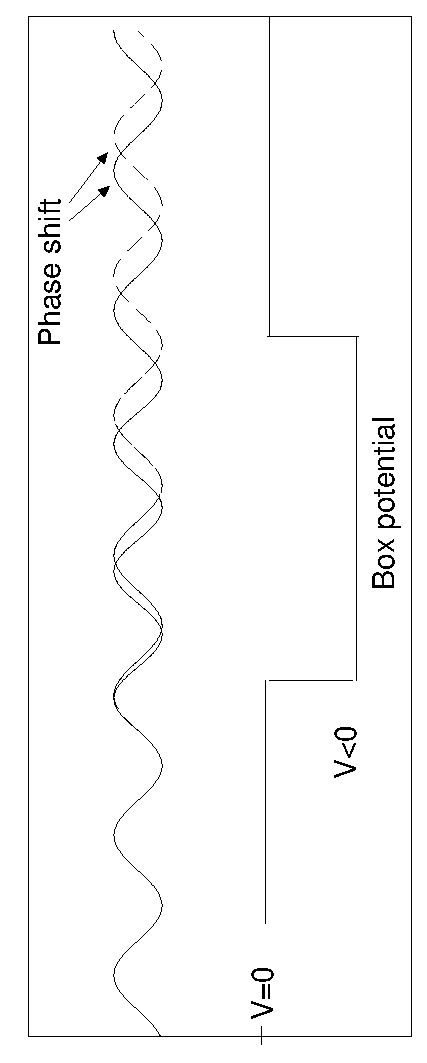
\includegraphics[height=15cm,angle=-90]{detteerfaseskift.eps}
\caption{Shows how a wave function will behave for a attractive box potential. The dashed line
illustrates the wave function behavior with out the potential.}
\end{figure}
\end{flushleft} 
However the phase shift can not be found directly. Experimentalist have to study the observable, 
which can be for example differential cross section and polarization. With these data, theorists are
able to calculate an NN-amplitude (A) for the process. This amplitude has many of the same properties as the S-matrix,
like the unitarian. In partial wave decomposition, it is related to the phase shift $\delta_l$ as
\begin{equation}
A_l=\eta_l e^{i2\delta_l}
\end{equation}

Inelasticity ($\eta_l$) is the probability amplitude for the scattering amplitude to be elastic. 
The inelasticity and phase shift are the necessary parameters to describe a partial wave. The inelasticity
becomes important for NN-scattering when the kinetic energy in the lab-system are above 350 MeV.
The inelasticity are due to energy released from the NN-system. This can be done by photon emission and/or particle
creations in the scattering.

  
%fig~\ref{fig:manypotS} shows the phase shift for different potentials and experimental phase shift.
%How the potentials are build up will be explained later.



\begin{flushleft} 

\begin{figure}\label{fig:manypotS}
\centering
\includegraphics[height=17cm]{manypotS.eps} 
\caption{\state{1}{S}{0} phase shifts for a box Potential, a parameterized potential, the Bonn B potential and
experimental data ~\cite{PRC48faseskift350MeV}. How the potentials are build up will be explained later.}
\end{figure}


\end{flushleft}




 %\headingx{Bibliografi}{}
 %\bibliography{ref.bib}
 %\include{bibliografi}
 %\headingx{Bibliografi}{}
 %\end{flushleft}

 %\cleardoublepage
 %\include{epilog}
 %\end{flushleft}
 \end{document}
 
